%%%%%%%%%%%%%%%%%%%%%%%%%%%%%%%%%%%%%%%%%%%%%%%%%%%%%%%%%%%%%%%%%%%
%%% Documento LaTeX 																						%%%
%%%%%%%%%%%%%%%%%%%%%%%%%%%%%%%%%%%%%%%%%%%%%%%%%%%%%%%%%%%%%%%%%%%
% Título:	Plantilla de PFC/TFG/TFM
% Autor:  Ignacio Moreno Doblas
% Fecha:  2014-02-01
%%%%%%%%%%%%%%%%%%%%%%%%%%%%%%%%%%%%%%%%%%%%%%%%%%%%%%%%%%%%%%%%%%%
% Compilador: 	MiKTeX 2.9.
%	Modo:					PDFLaTeX.
% Entorno:			TeXnicCenter 2.0 Stable Beta 2.
%%%%%%%%%%%%%%%%%%%%%%%%%%%%%%%%%%%%%%%%%%%%%%%%%%%%%%%%%%%%%%%%%%%

% Preámbulo del documento.
%-----------------------------------------------------------------%
% Clase de documento: libro
\documentclass[12pt,a4paper]{book} % article, report, book.

% Preámbulo: paquetes, comandos, entornos, estilos y título de página.
%%%%%%%%%%%%%%%%%%%%%%%%%%%%%%%%%%%%%%%%%%%%%%%%%%%%%%%%%%%%%%%%%%%
%%% Documento LaTeX 																						%%%
%%%%%%%%%%%%%%%%%%%%%%%%%%%%%%%%%%%%%%%%%%%%%%%%%%%%%%%%%%%%%%%%%%%
% Título:	Paquetes
% Autor:  Ignacio Moreno Doblas
% Fecha:  2014-02-01
%%%%%%%%%%%%%%%%%%%%%%%%%%%%%%%%%%%%%%%%%%%%%%%%%%%%%%%%%%%%%%%%%%%
% Tabla de materias:
%	1 Codificación e idioma %
% 2 Matemáticas y Física %
% 3 Gráficos%
% 4 Estilo y formato%
%%%%%%%%%%%%%%%%%%%%%%%%%%%%%%%%%%%%%%%%%%%%%%%%%%%%%%%%%%%%%%%%%%%

%1 Codificación e idioma%
\usepackage[utf8]{inputenc} %Codificación en latin-1%
\usepackage[spanish]{babel}	%Hyphenation (Guionado) en español%
\usepackage[T1]{fontenc} %Codificación de fuente%
%\usepackage{eurofont} %Tipografía euro (€)%

%2 Matemáticas y Física %
% Importante para ecuaciones, magnitudes y unidades%
\usepackage{amssymb,amsmath,latexsym,amsfonts} % paquetes estándar%
\usepackage[squaren]{SIunits} %Paquete para magnitudes y unidades físicas%
\usepackage{ifthen} %sentencias if y while%

%3 Gráficos%
\usepackage{graphics,graphicx} %paquetes gráficos estándar%
\usepackage{wrapfig} %paquete para gráfica lateral%
\usepackage[rflt]{floatflt} %figuras flotantes%
	% \begin{floatingfigure}[r]/[l]{4.5cm}
	% \end{floatingfigure}
\usepackage{graphpap}	%comando \graphpaper en el entorno picture%

%4 Estilo y formato%
\usepackage{placeins}
\usepackage{fancyhdr}	%cabeceras y pies mejor que con \pagestyle{}%
\usepackage{titlesec,titletoc} %Formateo de secciones y títulos%
\raggedbottom %Para fragmentar versos en varias páginas%
\usepackage{makeidx} %MakeIndex%
%\usepackage{showidx} % Hace que cada comando \index se imprima en la página donde se ha puesto (útil para corregir los índices)
\usepackage{alltt} % Define el environment alltt, como verbatim, excepto que \, { y } tienen su significado normal. Se describe en el fichero alltt.dtx.
\usepackage[pdftex,bookmarksnumbered,hidelinks]{hyperref} %hyper-references%
%\usepackage{minitoc} % Para poner tablas de contenido en cada capítulo.
\usepackage{listings} % Para escribir piezas de código C, Python, etc. %
%listings configuration
\lstset{
  language=Java, %Puede ser C, C++, Java, etc.
  showstringspaces=false,
  formfeed=\newpage,
  tabsize=4,
  commentstyle=\itshape,
  basicstyle=\ttfamily,
  morekeywords={models, lambda, forms}
}

\usepackage{mdframed}
\usepackage{footnote}
\usepackage{setspace}

\usepackage{moreverb}

%\usepackage{minted}
\usepackage[chapter]{minted}

\usepackage{tikz}
\usetikzlibrary{shapes, arrows}

\tikzstyle{block} = [rectangle, draw, fill=gray!20, 
    text width=5em, text centered, minimum height=4em]
\tikzstyle{line} = [draw, -latex']

\newcommand{\codigofuente}{\inputminted[linenos,numberblanklines,breaklines,frame=lines]}
%\newcommand{\codigfuente}{}

\newcommand{\extractocodigo}{\minted[linenos,numberblanklines,breaklines,frame=lines]}
%\newcommand{\codigfuente}{}

\usepackage{tipa} % tipografía IPA (International Phonetic Alphabet)
\usepackage{longtable} %Entorno Longtable, fracciona tablas a lo largo de páginas%
\usepackage{colortbl}
\usepackage{acronym}  %Para expandir automáticamente los acrónimos
%%%%%%%%%%%%%%%%%%%%%%%%%%%%%%%%%%%%%%%%%%%%%%%%%%%%%%%%%%%%%%%%%%%
%%% Documento LaTeX 																						%%%
%%%%%%%%%%%%%%%%%%%%%%%%%%%%%%%%%%%%%%%%%%%%%%%%%%%%%%%%%%%%%%%%%%%
% Título:	Comandos
% Autor:  Ignacio Moreno Doblas
% Fecha:  2014-02-01
%%%%%%%%%%%%%%%%%%%%%%%%%%%%%%%%%%%%%%%%%%%%%%%%%%%%%%%%%%%%%%%%%%%
% Tabla de materias:
% 1 Información del Documento %
% 2 Comandos a nivel de texto %
% 3 Comandos a nivel de entorno %
% 4 Comandos a nivel de página y sección %
% 5 Otros comandos %
%%%%%%%%%%%%%%%%%%%%%%%%%%%%%%%%%%%%%%%%%%%%%%%%%%%%%%%%%%%%%%%%%%%

% 1 Información del Documento %
\newcommand{\pfctitlename}{Título del Proyecto fin de Carrera}
\newcommand{\pfcauthorname}{Nombre del autor}
\newcommand{\pfctutorname}{Nombre del tutor}
\newcommand{\pfcanno}{año de publicación}

% 2 Comandos a nivel de texto %
\newcommand{\R}{\textsuperscript{\textregistered}}	%Símbolo registrado%
\newcommand{\C}{\textsuperscript{\copyright}}	%Símbolo Copyright%
\newcommand{\TM}{\texttrademark} %Símbolo Trade Mark (marca comercial)%

% 2.1 Comandos abreviatura %
\newcommand{\tit}{\textit} %Fuente cursiva (itálica)%
\newcommand{\tbf}{\textbf} %Fuente negrita%
\newcommand{\ttw}[1]{\texttt{#1}} %Fuente máquina de escribir (typewriter)%
%Combinación%
\newcommand{\textittt}[1]{\textit{\texttt{#1}}} %itálica y typewriter%
\newcommand{\textittw}{\textittt} % Otra forma de escribirlo.
\newcommand{\tittw}{\textittw} %Shortened%
\newcommand{\tbftw}[1]{\tbf{\ttw{#1}}}

%Crea una nueva línea y la indenta sin crear interlineado extra.
\newcommand{\nli}{\\ \indent} 

%Para escribir un correo electrónico%
\newcommand{\mailto}[1]{\href{mailto:#1}{#1}}

% Si vas a hacer un uso básico de \index (entradas en el índice de sólo un nivel, sin formatos especiales, etc.), define la orden
\newcommand{\miindex}[1]{#1\index{#1}}

\newcommand{\hs}{\hspace} % Abreviatura espacio horizontal
\newcommand{\vs}{\vspace} % Abreviatura espacio vertical

% Abreviaturas para los conjuntos de números más comunes.
\newcommand{\realnumbers}{\mathbb R}
\newcommand{\naturalnumbers}{\mathbb N}
\newcommand{\integernumbers}{\mathbb Z}
\newcommand{\rationalnumbers}{\mathbb Q}
\newcommand{\complexnumbers}{\mathbb R}
\newcommand{\irrationalnumbers}{\mathbb I}

% Doble barra sobre una letra (para expresar las matrices).
\newcommand{\doublebar}[1]{\bar{\bar{#1}}} 
% Ej: \vector(y) = \doublebar(A) \vector(x) (Stma. lineal de ec.)

% 3 Comandos a nivel de entorno %
\newcommand{\benu}{\begin{enu}} % Begin enumerate
\newcommand{\eenu}{\end{enu}} 	% End enumeration

%Comando para escribir código Python
\newcommand{\code}[3]{
  %\hrulefill
  %\subsection*{#1}
  %\subsubsection{#1}
  \lstinputlisting{#2}
  %#1\\
  \begin{table}[h!]
  	\centering
  	\caption{#1}
  	\label{#3}
  \end{table}
  \vspace{2em}
}

% 4 Comandos a nivel de página y sección %
%Crea página en blanco
\newcommand{\blankpage}{\clearpage{\pagestyle{empty}\cleardoublepage}}

% Versión x del comando section: sin numeración pero sí aparece en la tabla de contenidos.
\newcommand{\sectionx}[1]{
	\section*{#1}
	\addcontentsline{toc}{section}{#1}
}

% Versión y del comando section: sin numeración y NO aparece en la tabla de contenidos.
\newcommand{\sectiony}[1]{
	\section*{#1}
}

% Versión x del comando chapter: sin numeración pero sí  aparece en la tabla de contenidos.
\newcommand{\chapterx}[1]{
	\chapter*{#1}
	%\addcontentsline{toc}{chapter}{#1} %Caused by minitoc package%
	%\addstarredchapter{#1} %For minitoc package%
}

% substituto del comando \chapter: incluye estilo de página.
\newcommand{\chapterbegin}[1]%
	{%
		\pagestyle{fancy}
		\fancyhead[LE,RO]{\thepage}
		\fancyhead[LO]{Capítulo \thechapter. #1}
		%\fancyhead[RE]{Parte \thepart \rightmark} %
		\fancyhead[RE]{\nouppercase{\rightmark}} %
				
		\chapter{#1}
	}

% Versión x del comando \chapterbegin: sin numeración y aparece en la tabla de contenidos.
\newcommand{\chapterbeginx}[1]%
	{%
		\pagestyle{fancy}
		\fancyhead[RO,LE]{\thepage}
		\fancyhead[RE,LO]{#1}
		%\fancyhead[LO]{Chapter \thechapter}
		%\fancyhead[RE]{Part \thepart} %
		
		\chapterx{#1}
	}

%Fin de capítulo
\newcommand{\chapterend}{\pagestyle{empty}\cleardoublepage \thispagestyle{empty}}
%Si fuera un artículo en lugar un libro, \clearpage en lugar de \cleardoublepage

% 5 Otros comandos %
%\let\Oldpart\part
%\newcommand{\parttitle}{}
%\renewcommand{part}[1]{\Oldpart{#1}\renewcommand{\parttitle}{#1}} %Header customization%

%Cambiar el título índice de capítulo a ``Contenido''.
%\renewcommand{\mtctitle}{Contenido}

%\dominitoc % Para tablas de contenidos por capítulo.

\addto{\captionsspanish}{
	\renewcommand{\listtablename}{Índice de Tablas}
	\renewcommand{\tablename}{Tabla} } % Por ejemplo, modificar el nombre de 'Cuadro' a 'Tabla'.

\addto{\captionsspanish}{
	\renewcommand{\contentsname}{Índice} }
	
	\addto{\captionsspanish}{
	\renewcommand{\listingscaption}{Fragmento de código}}
	
	\addto{\captionsspanish}{
	\renewcommand{\listoflistingscaption}{Índice de fragmentos de código}}

\newcommand{\specialcell}[2][c]{%
  \begin{tabular}[#1]{@{}c@{}}#2\end{tabular}}
  
  \newcommand{\exedout}{%
  \rule{0.8\textwidth}{0.5\textwidth}%
}
%Si se desea cambiar el tipo de letra a Arial
% por cualquier razón, descomentar las siguientes
% dos líneas
%\renewcommand{\rmdefault}{phv} % Arial
%\renewcommand{\sfdefault}{phv} % Arial
	
%\addto{\captionsspanish}{
%	\renewcommand{\partname}{Fase} }

%\addto{\captionsspanish}{%
%    \renewcommand{\refname}{\vspace{-4.5ex}}} % Para que no aparezca el texto 'referencias' en la bibliografía.

% Modifica el interlineado
\renewcommand{\baselinestretch}{1.5}
%%%%%%%%%%%%%%%%%%%%%%%%%%%%%%%%%%%%%%%%%%%%%%%%%%%%%%%%%%%%%%%%%%%
%%% Documento LaTeX 																						%%%
%%%%%%%%%%%%%%%%%%%%%%%%%%%%%%%%%%%%%%%%%%%%%%%%%%%%%%%%%%%%%%%%%%%
% Título:	Entornos
% Autor:  Ignacio Moreno Doblas
% Fecha:  2014-02-01
%%%%%%%%%%%%%%%%%%%%%%%%%%%%%%%%%%%%%%%%%%%%%%%%%%%%%%%%%%%%%%%%%%%
% Tabla de materias:
%--------------------%
% 1 dobleindent
% 2 izqindent
% 3 dobleindentx
% 4 ite
% 5 descript
% 6 enu
% 7 itemization
% 8 sinopsis
%%%%%%%%%%%%%%%%%%%%%%%
% Para conocer los parámetros de diseño de las listas, tales como
%  los márgenes izquierdo, derechos y los diferentes saltos,
%  véase el archivo ``List layout.png'' que acompaña esta plantilla.
% Así se conocerá mejor cómo adaptar un entorno según los requisitos 
%  del usuario.

%%%%%%%%%%%%%%%%%%%%%%%
% Definición de longitudes para usar en los entornos:
%
% Normal parskip.
\newlength{\parskipenv}
\setlength{\parskipenv}{\parskip}

\newlength{\parindentenv}
\setlength{\parindentenv}{\parindent}
%%%%%%%%%%%%%%%%%%%%%%%

% 1 dobleindent
%El entorno dobleindent está pensando para escribir párrafos con doble indentación a cada lado.
%Tiene dos parámetros de entrada con las distancias medidas desde los márgenes de página.

\newenvironment{dobleindent}[2]
	%Comienzo de nuevo entorno%
	{
	\begin{list}
		{}
		{
		% Left and right margins:
		\leftmargin = #1 
		\rightmargin = #2
		%
		% Separation from preceding and following text:
		\topsep = 0ex
		\partopsep = 0ex
		\parsep = \parskipenv
		%
		% Indentation for paragraphs:
		\itemsep = \parskipenv
		\itemindent = \parindentenv
		\listparindent = \itemindent
		%
		% Horizontal separation from label:
		\labelsep = 1ex
		\settowidth{\labelwidth}{0cm}
		}
		
		 \item}
	% End new env
	{\end{list}}

%%%%%%%%%%%%%%%%%%%%%%%%%%%%%
%2 izqindent
% El entorno izqindent sólo crea un párrafo indentado a la izquierda.
\newenvironment{izqindent}[1]
{
\begin{dobleindent}{#1}{0cm}
}
{
\end{dobleindent}
}

%%%%%%%%%%%%%%%%%%%%%%%%%%%%%
% 3 dobleindentx
% El entorno dobleindentx es una variación del dobleindent usando leftskip y rightskip.
% Aunque es más limitado, también se puede usar.
\newenvironment{dobleindentx}[2] % Sólo funciona en modo paragraph
{ % Preamble
  \leftskip = #1
  \rightskip = #2
}
{ % Postamble
\leftskip = 0cm
\rightskip = 0cm
}

%%%%%%%%%%%%%%%%%%%%%%%%%%%%%
% 4 ite
% El entorno ite es una modificación del entorno itemize estándar de \LaTeX. Puede usarse o modificarse si el usuario lo desea.
% También puede parametrizarse el entorno enumerate o description de forma equivalente.
\newenvironment{ite}
	{
		\begin{izqindent}{\parindent}
		\hspace{-\parindent} 	% compensación del sangrado que introduce el entorno.
		\vspace{-1.0\parskip}	% compensación del \parskip que introduce el entorno.
		\vspace{-\baselineskip}	% compensación por la línea que introduce el entorno.
		\begin{itemize}
	}
	{
		\end{itemize}
		\end{izqindent}
	}

%%%%%%%%%%%%%%%%%%%%%5
% commando stdformat para formatear los entornos descript, enu y itemization.
\newcommand{\stdformat}
	{% Declarations for format presentation.
		%		  
		% Separation from preceding and following text:
		\setlength{\topsep}{0ex}%
		\setlength{\partopsep}{0ex} %
		%
		% Horizontal separation from label:
		\labelsep = 1ex
		\setlength{\labelwidth}{0ex}
		%
		%	Left and right margins:	
		\setlength{\leftmargin}{1cm}%
		\addtolength{\leftmargin}{\labelsep}
		\setlength{\rightmargin}{0ex}
		%  
		% Indentation for paragraphs:
		\setlength{\itemindent}{-\leftmargin}%
		\addtolength{\itemindent}{1ex}
		\setlength{\listparindent}{\parindent}%
		%		
		% Separation between paragraphs.
		\setlength{\parsep}{\parskipenv}% 
		\setlength{\itemsep}{1ex}
	}

%%%%%%%%%%%%%%%%%%%%%%%%%%%%%
% 5 descript

\newenvironment{descript}
	% Beginning new env def.
	{
		\begin{list}
			{} % No default label for \item.
			{
				% Declarations for format presentation.
				\stdformat
				%
				\renewcommand{\makelabel}[1]{\normalfont\bfseries##1\hfil}
			}
	}
	% Ending new env def.
	{
		\hspace*{\fill} \\ \end{list}
	} % Se introduce un salto de línea para que el texto siguiente esté separado.
%END newenvironment{descript}

%%%%%%%%%%%%%%%%%%%%%%%%%%%%%
% 6 enu
\newcounter{itemnumber} % Counter for the environment.

\newenvironment{enu}
	% Beginning new env def.
	{
		\begin{list}
		{
			\raggedleft \arabic{itemnumber}
		}
		{
			\usecounter{itemnumber}
			\stdformat
		}
	}
	{
		\end{list}
	}

%%%%%%%%%%%%%%%%%%%%%%%%%%%%%
% 7 itemization
\newenvironment{itemization}
	% Beginning new env def.
	{
		\begin{list}
			{$\bullet$} % No default label for \item.
			{
				% Declarations for format presentation.
				\stdformat
			}
	}
	% Ending new env def.
	{
		\end{list}
	}


%%%%%%%%%%%%%%%%%%%%%%%%%%%%%
% 8 sinopsis
\newenvironment{sinopsis}{%[1]{
	\sectiony{Sinopsis}
	%\label{#1}
} {
	\pagebreak
}
%%%%%%%%%%%%%%%%%%%%%%%%%%%%%%%%%%%%%%%%%%%%%%%%%%%%%%%%%%%%%%%%%%%
%%% Documento LaTeX 																						%%%
%%%%%%%%%%%%%%%%%%%%%%%%%%%%%%%%%%%%%%%%%%%%%%%%%%%%%%%%%%%%%%%%%%%
% Título:	Parámetros de estilo
% Autor:  Ignacio Moreno Doblas
% Fecha:  2014-02-01
%%%%%%%%%%%%%%%%%%%%%%%%%%%%%%%%%%%%%%%%%%%%%%%%%%%%%%%%%%%%%%%%%%%
% Tabla de materias:
%--------------------%
% 1 Márgenes de página
%%%%%%%%%%%%%%%%%%%%%%%
% Para conocer los parámetros de diseño de páginas, tales como
%  los márgenes izquierdo, derecho, anchura de página, etc.
%  véase el archivo ``Page layout.png'' que acompaña esta plantilla.
% Así se conocerá mejor cómo adaptar el documento según los 
%  requisitos del usuario.

% 1 Márgenes de página
%-------------------------------%
% Parámetros de estilo de página.
% DIN A4: 29.7 cm x 21 cm
%		área neta: 3 cm + 3 cm + 15 cm.
%
% Definición de márgenes de página
%  even para páginas pares
%  odd  para páginas impares
\newlength{\realoddsidemargin}	  % \oddsidemargin menos 1 in.
\newlength{\realevensidemargin}		% \evensidemargin menos 1 in.
\newlength{\realtopmargin}				% \topmargin menos 1 in.
%
% Asignación de márgenes de página
% ASIGNESE en caso de querer cambiarlo
\setlength{\realtopmargin}{2cm}			% REAL top margin.
\setlength{\realoddsidemargin}{3cm}		% REAL oddside margin.
\setlength{\realevensidemargin}{3cm}	% REAL evenside margin.
\setlength{\hoffset}{0cm}
\setlength{\voffset}{0cm}
%
% Substracción de 1 pulgada de compensación
%  (véase ``Page Layout.png'' para más información)
\addtolength{\realoddsidemargin}{-1in}	% 1 inch = 2.54 cm.
\addtolength{\realevensidemargin}{-1in}
\addtolength{\realtopmargin}{-1in}
%
% Asignación de anchuras y márgenes
% No hay notas al margen
\setlength{\marginparsep}{0cm} % No van a existir notas al margen
\setlength{\marginparwidth}{0cm} % No van a existir notas al margen
%
% Asignación de anchura de texto
\setlength{\textwidth}{15cm}	% Anchura neta del texto (globalmente).
%
% Asignación de márgenes par, impar y en altura
\setlength{\oddsidemargin}{\realoddsidemargin}	% odd-page left margin (global).
\setlength{\evensidemargin}{\realoddsidemargin}	% even-page left margin (global).
\setlength{\topmargin}{\realtopmargin}					% top margin (Global).

% Se puede usar también el paquete chngpage.

%%%%%%%%%%%%%%%%%%%%%%%%%%%%%%%%%%%%%%%%%%%%%%%%%%%%%%%%%%%%%%%%%%
%		1 Length commands.					%
%-------------------------------%
% Defines new length command (e.g., \newlength{\gnat}}
%	\newlength{}
%
% Set lenght to a value.
%	\setlength{\gnat}{length}
%	\addtolength{}{}
%
% Sets the value of a length command equal to the width of a specified piece of text; e.g., \settowidth{\parindent}{\em small}.
%	\settowidth{}{}
% Set the value of a height. e.g., \settoheight{\parskip}{Gnu}
%	\settoheight{}{}
% Set the value that extends below the line. e.g., \settodepth{\parskip}{gnu}.
%	\settodepth{}{}
%
% To multiply a length, write: 7.0\gnat = \gnat * 7.0
%%%%%%%%%%%%%%%%%%%%%%%%%%%%%%%%%%%%%%%%%%%%%%%%%%%%%%%%%%%%%%%%%%

%\interfootnotelinepenalty=10000

%Comando para crear glosario (index en inglés)
\makeindex


% Document body.
%-------------------------------------------------------------------%
\begin{document}
% Formato de documento hasta el capítulo 1 (sin incluirlo)
\frontmatter

%% Título y autor del proyecto
%%Rellenar con el nombre real del autor, título, tutor y año.
%%El departamento del tutor se escribe una vez en el Resumen del PFC
\renewcommand{\pfcauthorname}{Raúl Gómez Acuña}
\renewcommand{\pfctitlename}{SISTEMA DE MONITORIZACIÓN WEB DEL SISTEMA CARDIOVASCULAR MEDIANTE EL USO DEL PROTOCOLO BLUETOOTH 4.0 DE BAJA ENERGÍA}%
\renewcommand{\pfctutorname}{Álvaro Durán Martínez}
\renewcommand{\pfcanno}{2015}

% Los tres ficheros siguientes solamente deben descomentarse
%  en el caso de ser un PFC del plan a extinguir.
% En los nuevos títulos de grado, no exiten la portada, la calificación 
%  ni el Resumen del PFC.
% Estos tres documentos deben tomarse de la web de la ETSIT.
%
% Portada.
%%% Tipos de portada %%%
%	1. \maketitle
%	2. titlepage
%%%%%%%%%%%%%%%%%%%%%%%%

%	1. \maketitle
%%%%%%%%%%%%%%%%%%%%%%%%
%\maketitle
%\thispagestyle{empty}

%	2. titlepage
%%%%%%%%%%%%%%%%%%%%%%%%
\begin{spacing}{1}
\begin{titlepage}
	\begin{center}
		\Large{\textsc{\textsf{		Escuela Técnica Superior de Ingeniería de Telecomunicación Universidad de Málaga}}}
	\end{center}
	
	\bigskip
	 
	\begin{center}
		\begin{tabular}{lcr}
			%
\includegraphics[width=4cm,keepaspectratio]{graphs/EscudoETSIT.jpg} & \hspace{2cm}
			
\includegraphics[width=4cm,keepaspectratio]{graphs/EscudoETSIT.pdf} & \hspace{2cm}
			
\includegraphics[width=4cm,keepaspectratio]{graphs/UnivMalacitana.pdf}
		\end{tabular}
	\end{center}
	
	\bigskip
	
	\begin{center}\Large\textbf{\textsf{PROYECTO FIN DE CARRERA}}\end{center}
	
	\medskip
	
	\begin{center}
		\Huge
		\sffamily\scshape
		\pfctitlename
	\end{center}
	
	\medskip
	
	\begin{center}
		\Huge
		\scshape%\bfseries
		\textsf{Ingeniería de Telecomunicación}
	\end{center}
	
	\vfill
	
	{\large Málaga, \pfcanno \hfill \pfcauthorname}
	\blankpage
\end{titlepage}
\end{spacing}

% Hoja de calificación
\thispagestyle{empty}
\begin{spacing}{1}
\begin{center}
	\Large \sffamily \scshape %\bfseries
	Escuela Técnica Superior de\\
	Ingeniería de Telecomunicación\\
	Universidad de Málaga
\end{center}

	{\bfseries \noindent Titulación: Ingeniería de Telecomunicación \\
	}\\[3ex]

	\noindent Reunido el tribunal examinador en el día de la fecha, constituido por:\\[3ex]
	\textbf{D./Dª.~}\hrulefill\\[3ex]
	\textbf{D./Dª.~}\hrulefill\\[3ex]
	\textbf{D./Dª.~}\hrulefill\\[3ex]
	
	para juzgar el Proyecto Fin de Carrera titulado:\noindent 
	
\begin{center}
	\large \bfseries \pfctitlename
\end{center}

\noindent del alumno \tit{D./Dª.~\pfcauthorname}

\noindent dirigido por \tit{D./Dª.~\pfctutorname}

\bigskip

	\noindent ACORDÓ POR \hrulefill OTORGAR LA\\[3ex]%\rule{3cm}{0.1mm} otorgar la\\[3ex]
	CALIFICACIÓN DE\hrulefill\\[3ex]
	
	%\hrulefill\\[3ex]
	
	\noindent y, para que conste, se extiende firmada por los componentes del tribunal, la presente diligencia.
	
	\bigskip

\hfill Málaga, a \rule{1cm}{0.1mm} de \rule{1cm}{0.1mm} de \rule{0.7cm}{0.1mm}

\vskip 10pt

\begin{center}
	\begin{tabular}{ccc}
	El Presidente: & El Vocal: & El Secretario:\\[2cm]
	Fdo.:\rule{3cm}{0.1mm} & Fdo.:\rule{3cm}{0.1mm} & Fdo.:\rule{3cm}{0.1mm}	
	\end{tabular}
\end{center}
\end{spacing}
\blankpage

% Resumen del proyecto (formulario)
%%%%%%%%%%%%%%%%%%%%%%%%%%%%%%%%%%
% Página de resumen del proyecto %
%%%%%%%%%%%%%%%%%%%%%%%%%%%%%%%%%%

\thispagestyle{empty}
\begin{spacing}{1}

\begin{center}
	\Large \sffamily
	Universidad de Málaga\\
	Escuela Técnica Superior de Ingeniería de\\
	Telecomunicación
\end{center}

\bigskip

\begin{center}
	\Huge\scshape
	\pfctitlename
\end{center}

\bigskip

\begin{center}
	\textbf{REALIZADO POR}\\
	\textsf{\pfcauthorname}
\end{center}

\medskip

\begin{center}
	\textbf{DIRIGIDO POR}\\
	\textsf{\pfctutorname}
\end{center}

\vfill

\begin{minipage}{\textwidth}
\textbf{Dpto. de:} Ingeniería de Comunicaciones (IC)

\medskip

\textbf{Palabras clave:} Bluetooth, Android, aplicación, localización, web, corazón

\medskip

\textbf{Titulación:} Ingeniería de Telecomunicación

\medskip

\textbf{Resumen:}	
	El presente proyecto pretende realizar una prueba de concepto sobre el diseño e implementación de un sistema de monitorización del ritmo cardíaco, a través del conjunto de dos aplicaciones, una aplicación Android que se conectará y recibirá datos del sensor mediante el protocolo Bluetooth 4.0 de baja energía, transmitiendo dichos datos a un servidor web y una aplicación web, que usará una conexión web socket para mostrar los datos en tiempo real

\begin{center} Málaga, \today\end{center}
\end{minipage}
\end{spacing}
\blankpage

% Dedicatoria.
%%%%%%%%%%%%%%%%%%%%%%%%%%%%%%%%%%%%%%%%%%%%%%%%%%%%%%%%%%%%%%%%%%%
%%% Documento LaTeX 																						%%%
%%%%%%%%%%%%%%%%%%%%%%%%%%%%%%%%%%%%%%%%%%%%%%%%%%%%%%%%%%%%%%%%%%%
% Título:	Dedicatoria
% Autor:  Ignacio Moreno Doblas
% Fecha:  2014-02-01
%%%%%%%%%%%%%%%%%%%%%%%%%%%%%%%%%%%%%%%%%%%%%%%%%%%%%%%%%%%%%%%%%%%
% Esta plantilla sirve para dedicatoria.

\cleardoublepage
\thispagestyle{empty} % No queremos mostrar ningún encabezamiento ni pie de página.

\begin{minipage}[c][\textheight][c]{\textwidth} %[pos][height][inner-pos]{width}
\raggedleft %\flushleft

Este Proyecto Fin de Carrera está dedicado a mis padres, por su apoyo incondicional durante esta larga etapa, y que sin duda han sido pieza clave para llegar hasta donde estoy

\bigskip

\emph{El autor}

\end{minipage}

\blankpage

% Acrónimos
%%%%%%%%%%%%%%%%%%%%%%%%%%%%%%%%%%%%%%%%%%%%%%%%%%%%%%%%%%%%%%%%%%%
%%% Documento LaTeX 																						%%%
%%%%%%%%%%%%%%%%%%%%%%%%%%%%%%%%%%%%%%%%%%%%%%%%%%%%%%%%%%%%%%%%%%%
% Título:	Lista de acrónimos
% Autor:  Ignacio Moreno Doblas
% Fecha:  2014-02-01
%%%%%%%%%%%%%%%%%%%%%%%%%%%%%%%%%%%%%%%%%%%%%%%%%%%%%%%%%%%%%%%%%%%

%Lista de acrónimos 
\chapterbeginx{Acrónimos}

\begin{acronym}[DLMS/COSEMM]
	\acro{AFH}{Adaptive Frequency Hoping, o espectro ensanchado adaptable con salto de frecuencia}
	\acro{AJAX}{Asynchronous Javascript And XML, o JavaScript asíncrono y XML}
	\acro{AMD}{Asynchronous Module Definition, o definición asíncrona de módulos}
	\acro{ATT}{Attribute Protocol, o protocolo de atributo}
	\acro{API}{Application Programming Interface, o interfaz de programación de aplicaciones}
	\acro{BLE}{Bluetooth Low Energy, o Bluetooth de baja energía}
	\acro{CMOS}{Complementary Metal Oxide Semiconductor, o semiconductor complementario de óxido metálico}
	\acro{CSS}{Cascading Style Sheets, o hoja de estilo en cascada}
	\acro{DOM}{Document Object Model, o modelo de objetos del documento}	
	\acro{DSL}{Domain Specific Language, o lenguaje específico del dominio}
	\acro{EDR}{Enhanced Data Rate, o velocidad de transmisión de datos mejorada}
	\acro{ETSIT}{Escuela Técnica Superior de Ingeniería de Telecomunicación}
	\acro{GATT}{Generic Attribute Profile, o Perfil de Atributo Genérico}
	\acro{GMS}{Google Mobile Services, o servicios móviles de Google}
	\acro{GPS}{Global Positioning System, o sistema de posicionamiento global}
	\acro{HAL}{Hardware Abstraction Layer, o capa de abstracción del hardware}
	\acro{HTML}{HyperText Markup Language, o lenguaje de marcas de hipertexto}
	\acro{IDE}{Integrated Development Environment, o entorno de desarrollo integrado}
	\acro{ISM}{Industrial, Scientific and Medical, o industrial, científico y médico}
	\acro{JNI}{Java Native Interface, o interfaz nativa Java}
	\acro{JSON}{JavaScript Object Notation, o notación de objetos de JavaScript}
	\acro{MAC}{Media Access Control, o control de acceso al medio}
	\acro{MVC}{Model-View-Controller, o modelo-vista-controlador}
	\acro{PCB}{Printed Circuit Board, o placa de circuito impreso}
	\acro{PFC}{Proyecto Fin de Carrera}
	\acro{POO}{Programación Orientada a Objetos}
	\acro{RAM}{Random Access Memory, o memoria de acceso aleatorio}
	\acro{RSSI}{Received Signal Strength Indicator, o indicador de fuerza de la señal recibida}
	\acro{SIG}{Special Interest Group, o grupo de especial interés}	
	\acro{SVG}{Scalable Vector Graphics, o gráficos vectoriales escalables}
	\acro{TDD}{Time-Division Duplexing, o duplexación por división de tiempo}
	\acro{UMA}{Universidad de Málaga}
	\acro{URL}{Uniform Resource Locator, o localizador de recursos uniforme}
	\acro{UUID}{Universally Unique Identifier, o identificador universal único}
	\acro{XML}{eXtensible Markup Language, o lenguaje de marcado extensible}
\end{acronym}

\chapterend

% Tabla de contenidos, figuras y tablas.
%%%%%%%%%%%%%%%%%%%%%%%%%%%%%%%%%%%%%%%%%%%%%%%%%%%%%%%%%%%%%%%%%%%
%%% Documento LaTeX 																						%%%
%%%%%%%%%%%%%%%%%%%%%%%%%%%%%%%%%%%%%%%%%%%%%%%%%%%%%%%%%%%%%%%%%%%
% Título:	Índice (Tabla de contenidos)
% Autor:  Ignacio Moreno Doblas
% Fecha:  2014-02-01
%%%%%%%%%%%%%%%%%%%%%%%%%%%%%%%%%%%%%%%%%%%%%%%%%%%%%%%%%%%%%%%%%%%

%\pagestyle{fancy}

%\dominitoc %Este comando es para el índice por capítulo%

\tableofcontents

%\fancyhead[RO,LE]{\roman{page}} %El contador page no lleva \
%\fancyhead[LO,RE]{Tabla de Contenidos}
%\fancyhead[RE,LO]{\nouppercase{\rightmark}}
%\fancyfoot[C]{}

%\dottedcontents{part}[1em]{\bfseries \large Part }{0em}{1pc}
%\dottedcontents{chapter}[0.5cm]{\ }{1em}{1pc}
%\titlecontents{chapter}[2em]{}{Chapter \thecontentslabel}{}{\\}
%\dottedcontents{chapter}[2.5em]{Chapter }{0em}{1pc}

\chapterend

%%%%%%%%%%%%%%%%%%%%%%%%%%%%%%%%%%%%%%%%%%%%%%%%%%%%%%%%%%%%%%%%%%%
%%% Documento LaTeX 																						%%%
%%%%%%%%%%%%%%%%%%%%%%%%%%%%%%%%%%%%%%%%%%%%%%%%%%%%%%%%%%%%%%%%%%%
% Título:	Índice de Figuras (Tabla de Figuras)
% Autor:  Ignacio Moreno Doblas
% Fecha:  2014-02-01
%%%%%%%%%%%%%%%%%%%%%%%%%%%%%%%%%%%%%%%%%%%%%%%%%%%%%%%%%%%%%%%%%%%

\pagestyle{fancy}

\listoffigures
\fancyhead[RO,LE]{\roman{page}} %El contador page no lleva \

\fancyhead[RE,LO]{\nouppercase{\rightmark}}

\chapterend
%%%%%%%%%%%%%%%%%%%%%%%%%%%%%%%%%%%%%%%%%%%%%%%%%%%%%%%%%%%%%%%%%%%
%%% Documento LaTeX 																						%%%
%%%%%%%%%%%%%%%%%%%%%%%%%%%%%%%%%%%%%%%%%%%%%%%%%%%%%%%%%%%%%%%%%%%
% Título:	Índice de Figuras (Tabla de Figuras)
% Autor:  Ignacio Moreno Doblas
% Fecha:  2014-02-01
%%%%%%%%%%%%%%%%%%%%%%%%%%%%%%%%%%%%%%%%%%%%%%%%%%%%%%%%%%%%%%%%%%%

\pagestyle{fancy}

\listoflistings
\fancyhead[RO,LE]{\roman{page}} %El contador page no lleva \

\fancyhead[RE,LO]{\nouppercase{\rightmark}}

\chapterend
%%%%%%%%%%%%%%%%%%%%%%%%%%%%%%%%%%%%%%%%%%%%%%%%%%%%%%%%%%%%%%%%%%%
%%% Documento LaTeX 																						%%%
%%%%%%%%%%%%%%%%%%%%%%%%%%%%%%%%%%%%%%%%%%%%%%%%%%%%%%%%%%%%%%%%%%%
% Título:	Índice de Tablas (Tabla de Tablas)
% Autor:  Ignacio Moreno Doblas
% Fecha:  2014-02-01
%%%%%%%%%%%%%%%%%%%%%%%%%%%%%%%%%%%%%%%%%%%%%%%%%%%%%%%%%%%%%%%%%%%

\pagestyle{fancy}

\listoftables

\fancyhead[RO,LE]{\roman{page}}
\fancyhead[RE,LO]{\nouppercase{\rightmark}}

\chapterend

% Formato de documento durante los capítulos.
\mainmatter

% Prólogo.
%%%%%%%%%%%%%%%%%%%%%%%%%%%%%%%%%%%%%%%%%%%%%%%%%%%%%%%%%%%%%%%%%%%%
%%% Documento LaTeX 																						%%%
%%%%%%%%%%%%%%%%%%%%%%%%%%%%%%%%%%%%%%%%%%%%%%%%%%%%%%%%%%%%%%%%%%%
% Título:	Prólogo
% Autor:  Ignacio Moreno Doblas
% Fecha:  2014-02-01
%%%%%%%%%%%%%%%%%%%%%%%%%%%%%%%%%%%%%%%%%%%%%%%%%%%%%%%%%%%%%%%%%%%

\chapterbeginx{Prólogo}

%\minitoc
	El presente proyecto consiste en desarrollar una aplicación móvil para el sistema operativo Android, cuya funcionalidad es la medición del nivel de ruido asociado a un punto geográfico, y la representación del mismo superpuesto a un mapa geográfico.


\chapterend

% Parte I. Introducción
\part{Introducción}

% Introducción y objetivo
%%%%%%%%%%%%%%%%%%%%%%%%%%%%%%%%%%%%%%%%%%%%%%%%%%%%%%%%%%%%%%%%%%%
%%% Documento LaTeX 																						%%%
%%%%%%%%%%%%%%%%%%%%%%%%%%%%%%%%%%%%%%%%%%%%%%%%%%%%%%%%%%%%%%%%%%%
% Título:		Introducción
% Autor:  	Ignacio Moreno Doblas
% Fecha:  	2014-02-01
% Versión:	0.5.0
%%%%%%%%%%%%%%%%%%%%%%%%%%%%%%%%%%%%%%%%%%%%%%%%%%%%%%%%%%%%%%%%%%%

%\chapterbeginx{Introducción, Objetivo y Visión general}
\chapterbeginx{Introducción y visión general}
%\minitoc

\sectionx{Presentación del Proyecto}
\label{sec:intro:obj}
	Este proyecto es fundamentalmente una prueba de concepto. Para los desconocidos del término podemos resumir en breves palabras que se trata del diseño e implementación de un prototipo, con el propósito de verificar que el concepto es susceptible de ser explotado de una manera útil.
	
	Nos hemos atrevido con una idea interesante, y a su vez desafiante, como resulta ser un sistema de monitorización del sistema cardiovascular en tiempo real, y usando unos recursos muy simples y al alcance de cualquiera, como son el uso de un pulsómetro comercial con Bluetooth integrado de última generación y un teléfono inteligente Android. Se ha desarrollado una aplicación Android, la cual recibirá datos transmitidos por el pulsómetro mediante el protocolo Bluetooth 4.0, en su modo de baja energía, y enviará dichos datos a un servidor web a través del método POST del protocolo HTTP.
	
	En este prototipo el término ``tiempo real'' es el aspecto clave, puesto que el objetivo es que cualquier persona (en un principio) sea capaz de ver inmediatamente reflejado en la web el último valor de frecuencia cardíaca detectado por el pulsómetro. En otras palabras, usted se encuentra realizando ejercicio en el exterior con el pulsómetro atado al pecho y con su teléfono móvil Android en el bolsillo, y cualquier persona interesada, por ejemplo un doctor, podría consultar en directo su ritmo cardiovascular y ver dicha evolución en una gráfica desde cualquier dispositivo móvil con acceso a Internet.
	
	Sin embargo, para tal propósito nos falta la otra pieza del puzzle para que todo encaje perfectamente: conexiones de baja latencia cliente-servidor y servidor-cliente, siendo el servidor un servidor web el cual implementaremos desde cero y tendremos total control sobre él, y cliente cualquier navegador web. ¿Se preguntan cómo conseguir dicha baja latencia? Los Web Sockets nos abren el camino.
	
	La figura \ref{figure:esquemaIntro} provee una visión general del sistema que se ha implementado.
	
	\begin{figure}[!htbp] \centering
		\includegraphics[height=20cm]{graphs/esquemaIntroductorio.pdf}
		\caption{Sistema de monitorización del ritmo cardíaco (visión general)}
		\label{figure:esquemaIntro} 
	\end{figure}
    

\sectionx{Motivación}
    Entre los tecnólogos, la salud móvil está en auge. Según estudios del Instituto Tecnológico de Massachusetts, desde principios de 2013 se han invertido más de 550 millones de euros en capital riesgo en empresas para crear productos de salud móvil e invirtiendo en \tit{start-ups}.
    
    La idea es simple: cada vez hay más teléfonos inteligentes, lo que significa que el uso generalizado de sensores pequeños y baratos, Bluetooth de baja energía y software de análisis permitirán que pacientes y médicos registren todo tipo de datos para mejorar la atención médica.
    
    Con el lanzamiento de la versión 4.3 a mediados de 2013, Android introdujo la compatibilidad con Bluetooth 4.0 y su modo de baja energía. Esto hecho abrió la puerta a poder conectar sensores a aplicaciones Android, como por ejemplo medidores de frecuencia cardíaca, los cuales pueden adquirirse por un precio que ronda los 30-40 euros y proporcionan una alta precisión en la medida.
    
    La combinación de leer y almacenar datos de sensores en nuestro dispositivo Android, junto con un acceso completo a Internet desde este, nos garantiza un mundo lleno de posibilidades en el campo de la monitorización, poniendo esos datos a disponibilidad de un amplio público, todo ello en tiempo real gracias a la experiencia que la web nos brinda.
\sectionx{Estado del arte}
    La explosión  que el desarrollo web ha sufrido en los últimos años, proporcionando notables avances tecnológicos como NodeJS (JavaScript del lado del servidor), pilas o \tit{stacks} de desarrollo web completo como MEAN (usando Javascript cómo único lenguaje en todo la pila) e implementaciones de Web Sockets usando JavaScript y NodeJS, ha conseguido que podamos desarrollar ricas aplicaciones web en menor cantidad de tiempo y con una menor complejidad técnica.
    
    Por otra parte, la penetración de mercado de los teléfonos inteligentes crece día a día, superando 1.75 mil millones de usuarios para final de 2014\cite{smartphoneusers}. Como se observa en la tabla \ref{tab:mobileusage}, cerca de dos quintos de la base total de usuarios de teléfonos móviles, utiliza teléfonos móviles inteligentes. Esto supone cerca de un cuarto de la población mundial.

\begin{table}[H]%
\centering
\begin{tabular}{|c|c|c|c|c|c|c|}
    \hline
    \hline
    \tbf{}&\tbf{2012} &\tbf{2013}&\tbf{2014}&\tbf{2015}&\tbf{2016}&\tbf{2017}\\ \hline 
    \tbf{\specialcell{ Usuarios totales \\ (miles de millones)}}&1.13&1.43&1.75&2.03&2.28&2.50 \\ \hline
    \tbf{\% de incremento}&68.4\%&27.1\%&22.5\%&15.9\%&12.3\%&9.7\%\\ \hline
    \tbf{\% de usuarios móviles}& 27.6\%&33.0\%&38.5\%&42.6\%&46.1\%&48.8\%\\ \hline
    \tbf{\% de población mundial}&16.0\%&20.2\%&24.4\%&28.0\%&31.2\%&33.8\% \\ \hline
    \hline 
\end{tabular}
\caption{Usuarios de teléfonos móviles inteligentes \cite{smartphoneusers}}\label{tab:mobileusage}
\end{table} 

    Dentro del segmento de usuarios de teléfonos móviles inteligentes, existen varios sistemas operativos móviles, cada cual provee su propia plataforma de desarrollo, entorno de desarrollo y ecosistema de aplicaciones. A raíz de la información de la tabla \ref{tab:mobimarketshare}, se observa que Android es el líder del mercado, con sobrada ventaja.

 \begin{table}[H]%
\centering
\begin{tabular}{|c|c|c|c|c|c|}
    \hline
    \hline
\tbf{Período}&\tbf{Android}&\tbf{iOS}&\tbf{Windows Phone}&\tbf{BlackBerry OS}&\tbf{Otros}\\
\tbf{T3 2014}&84.4\%&11.7\%&2.9\%&0.5\%&0.6\%\\
\tbf{T3 2013}&81.2\%&12.8\%&3.6\%&1.7\%&0.6\%\\
\tbf{T3 2012}&74.9\%&14.4\%&2.0\%&4.1\%&4.5\%\\
\tbf{T3 2011}&57.4\%&13.8\%&1.2\%&9.6\%&18.0\%\\
\hline
    \hline 
    \end{tabular}
\caption{Cuota de mercado de los distintos sistemas operativos móviles \cite{smartphonemarket}}\label{tab:mobimarketshare}
\end{table} 
    % situacion actual con relativo detalle 
    
\sectionx{Herramientas y metodologías utilizadas}
Para el desarollo de la aplicación Android, la principal herramienta utilizada ha sido el entorno de desarrollo integrado Android Studio. Es un entorno de relativa novedad, ya que aunque su primera versión estable fue liberada en Diciembre de 2014, su desarrollo se remonta a Mayo de 2013. Android Studio está disponible de manera gratuita para las plataformas mayoritarias Windows, Mac OS X y Linux. Al ser un entorno de desarrollo enfocado completamente al ecosistema Android, provee múltiples ayudas y mejoras sobre un entorno de desarrollo integrado más genérico como puede ser Eclipse. Características que han hecho decantarse por Android Studio y no Eclipse se analizan en el apartado \ref{sec:IDE}.

Para el desarrollo de la aplicación web, se ha recurrido al editor de texto gratuito y de código fuente abierto Atom.
Es un entorno áltamente personalizable que explota lo mejor de los editores más populares del mercado.

Ha sido necesario también un teléfono inteligente con Android, tanto durante la fase de desarrollo como durante las posteriores de utilización y realización de pruebas, así como un ordenador portátil Macbook Pro, actuando como servidor web durante la fase de desarrollo.

\sectionx{Estructura del documento}

\begin{description}

\item[Introducción teórica]\hfill \\
En el capítulo 1 se hará una introducción a los conceptos teóricos requeridos para la comprensión del trabajo realizado.
Se explicará el protocolo Bluetooth y su versión de baja energía.
A su vez, también se explicarán conceptos relativos a la programación en Android, tratados a lo largo del proyecto.
Por último se realizará una breve introducción al desarrollo de aplicaciones web modernas, haciendo hincapié en el \tit{stack} MEAN, ya que ha sido el utilizado en el presente proyecto.

\item[Implementación]\hfill \\
En el capítulo 2 se explicará cómo se ha llevado a cabo toda la implementación de la aplicación, empezando por un análisis de los requisitos necesarios para la realización de esta, y siguiendo con los aspectos relevantes a la programación de la aplicación tanto Android como Web: métodos, interfaz gráfica, diagramas de flujo, algoritmos, etc.

\item[Plan de pruebas y verificación] \hfill \\
En el capítulo 3 se explicarán los procedimientos llevados a cabo para cerciorar el correcto funcionamiento de la aplicación.

\item[Conclusiones y trabajo futuro] \hfill \\
En este apartado se pretende representar las conclusiones obtenidas durante la realización de este proyecto, así como plasmar posibles ideas que se consideran interesantes de cara a una futura continuidad en el desarrollo de la aplicación.

\end{description}


\chapterend{}


\part{Desarrollo del proyecto}

% Capítulo 01.
%%%%%%%%%%%%%%%%%%%%%%%%%%%%%%%%%%%%%%%%%%%%%%%%%%%%%%%%%%%%%%%%%%%
%%% Documento LaTeX 																						%%%
%%%%%%%%%%%%%%%%%%%%%%%%%%%%%%%%%%%%%%%%%%%%%%%%%%%%%%%%%%%%%%%%%%%
% Título:		Capítulo 1
% Autor:  	Ignacio Moreno Doblas
% Fecha:  	2014-02-01
% Versión:	0.5.0
%%%%%%%%%%%%%%%%%%%%%%%%%%%%%%%%%%%%%%%%%%%%%%%%%%%%%%%%%%%%%%%%%%%
\chapterbegin{Introducción teórica}
%\minitoc

%\begin{sinopsis}
%\label{sec:chpltx:sinop}
%	
%\end{sinopsis}

\section{Bluetooth}
\label{sec:Bluetooth}


\subsection{Historia}

	En 1994 Ericsson inició un estudio para investigar la viabilidad de un sistema de comunicaciones vía radio, de bajo coste y bajo consumo, para la interconexión entre teléfonos móviles y otros accesorios con la intención de eliminar cables entre aparatos. El estudio partía de un largo proyecto que investigaba sobre unos dispositivos transceptores conectados a una red celular, hasta llegar a un enlace de radio de corto alcance, llamado \tit{MC link}.

	Conforme este proyecto avanzaba, se empezó a visualizar que este tipo de enlace podía ser utilizado ampliamente en un gran número de aplicaciones, ya que tenía como principal virtud el basarse en un chip de radio relativamente económico. 
 
	A comienzos de 1997, según avanzaba el proyecto \tit{MC link}, Ericsson fue despertando el interés de otros fabricantes de equipos portátiles. De seguida se vio claramente que para que el sistema tuviera éxito un gran número de equipos deberían estar equipados con esta tecnología. Esto fue lo que llevó, a principios de 1998, a crear un \ac{SIG}, formado por 5 promotores que eran: Ericsson, Nokia, IBM, Toshiba e Intel. La idea era lograr un conjunto adecuado de áreas de negocio, dos líderes del mercado de las telecomunicaciones, dos líderes del mercado de los ordenadores portátiles y un líder de la fabricación de chips. A día de hoy hay más de 20.000 empresas que lo conforman.

	Obviamente Bluetooth no se llamó así desde un comienzo. El origen surge en 1994, cuando uno de los desarrolladores, Jim Kardach, propuso el nombre de uno de los reyes vikingos, específicamente el de Harald Blåtand, cuya traducción al inglés es Harald Bluetooth.
	
	Este rey fue conocido por unificar las tribus noruegas, suecas-danesas y por convertirlas al cristianismo, que en paralelo es la fusión de la comunicación de los sistemas digitales, que buscaba reemplazar el cable para los dispositivos móviles.
	

\begin{figure}[h] \centering
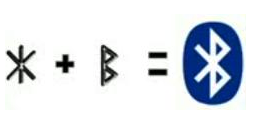
\includegraphics[width=6cm]{graphs/bluetooth_logo.png} 
\caption{Origen del logotipo comercial de Bluetooth \cite{bluetoothoficial}}
\label{bluetoothOrigin}
\end{figure}

	Aún hay más misterios escandinavos relacionados con la tecnología como cuál es el origen del logotipo. El logotipo es una combinación de dos letras del alfabeto rúnico, precisamente la H y la B. Dicha fusión se aprecia en la figura \ref{bluetoothOrigin}.

\subsection{Usos y aplicaciones }\label{cap:usosAplicaciones}
	Se denomina Bluetooth a la norma que define un estándar global de comunicación inalámbrica, que posibilita la transmisión de voz y datos entre diferentes equipos mediante un enlace por radiofrecuencia. Los principales objetivos que se pretende conseguir con esta norma son: facilitar las comunicaciones entre equipos móviles y fijos, eliminar cables y conectores entre estos, ofreciendo la posibilidad de crear pequeñas redes inalámbricas y facilitar la sincronización de datos entre nuestros equipos personales.
	
	Los dispositivos que incorporan este protocolo pueden comunicarse entre sí cuando se encuentran dentro de su radio de alcance. Las comunicaciones se realizan por radiofrecuencia de forma que los dispositivos no tienen que estar alineados y pueden incluso estar en habitaciones separadas si la potencia de transmisión es suficiente. Estos dispositivos se clasifican como Clase 1, Clase 2 o Clase 3 en referencia a su potencia de transmisión, tal y como muestra la tabla \ref{bluetoothTable}

\begin{table}[H]%
	\centering
\begin{tabular}{|c|c|c|c|}
	\hline
	\hline
	\tbf{Clase}&\tbf{\specialcell{Potencia máxima \\ permitida (mW)}} &\tbf{\specialcell{Potencia máxima \\ permitida (dBm)}}&\tbf{\specialcell{Alcance \\ (aproximado)}}\\ \hline 
	\tbf{Clase 1}&100 mW&20 dBm&100 metros\\ \hline
	\tbf{Clase 2}&2.5 mW&4 dBm&5-10 metros\\ \hline
	\tbf{Clase 3}&1 mW&0 dBm&1 metro\\ \hline
	\hline 
\end{tabular}
\caption{Clases de dispositivos Bluetooth \cite{wikibluetooth}}
\label{bluetoothTable}
\end{table} 

	Para utilizar Bluetooth, un dispositivo debe implementar alguno de los perfiles Bluetooth.
	Los perfiles son descripciones de comportamientos generales que los dispositivos pueden utilizar para comunicarse, formalizados para favorecer un uso unificado. La forma de utilizar las capacidades de Bluetooth se basa, por tanto, en los perfiles que soporta cada dispositivo. Los perfiles permiten la manufactura de dispositivos que se adapten a sus necesidades. Ejemplos de estos son el perfil \tit{File Transfer Profile}  (FTP) para la transferencia de ficheros a través de Bluetooth, o el perfil \tit{Advanced Audio Distribution Profile} (A2DP), el cual define cómo se puede propagar un flujo de audio (mono o estéreo) entre dispositivos a través de una conexión Bluetooth.

\subsubsection{Aplicaciones}
\begin{itemize}
	
	\item Conexión sin cables para el intercambio de datos.
	\item Transferencia de fichas de contactos, citas y recordatorios entre dispositivos.
	\item Reemplazo de la tradicional comunicación por cable entre equipos GPS y equipamiento médico.
	\item Controles remotos (tradicionalmente dominado por el infrarrojo).
	\item Enviar pequeñas publicidades desde anunciantes a dispositivos con Bluetooth. Un negocio podría enviar publicidad a teléfonos móviles cuyo Bluetooth (los que lo posean) estuviera activado al pasar cerca
	\item Enlace inalámbrico entre sistemas de audio y los altavoces correspondientes.
	\item Controladores remotos inalámbricos para videojuegos.
	
\end{itemize}


\subsection{Especificaciones}


\subsubsection{La tecnología}

La especificación de Bluetooth define un canal de comunicación de máximo 720 kbps (kilobits por segundo) con un rango óptimo de 10 metros (opcionalmente 100 m con repetidores).

Para poder operar en todo el mundo es necesaria una banda de frecuencia abierta a cualquier sistema de radio independientemente del lugar del planeta donde nos encontremos. Sólo la banda \ac{ISM} de 2,45 GHz cumple con este requisito, con rangos que van de los 2.400 MHz a los 2.480 MHz, con algunas restricciones en países como Francia, España y Japón. 

Para evitar interferencias, ya que la banda \ac{ISM} está abierta a cualquiera, se utiliza el sistema de salto de frecuencia. Este sistema divide la banda de frecuencia en varios canales de salto donde los transceptores, durante la conexión, van cambiando de uno a otro de manera pseudo-aleatoria, consiguiendo que el ancho de banda instantáneo sea muy pequeño y también una propagación sobre el total de la banda. 

El canal pues, queda dividido en intervalos de 625 $\mu$s, llamados ranuras o \tit{slots}, donde cada salto de frecuencia es ocupado por una ranura}. Esto da lugar a una frecuencia de salto de 1600 veces por segundo. Un paquete de datos puede ocupar una ranura para la emisión y otro para la recepción y pueden ser usados alternativamente, dando lugar a un esquema de tipo \ac{TDD}. Los saltos de frecuencia se dan entre un total de 79 frecuencias con intervalos de 1MHz, proporcionando seguridad y robustez.

La potencia de salida para transmitir a una distancia máxima de 10 metros es de 0 dBm (1 mW), mientras que la versión de largo alcance transmite entre 20 y 30 dBm (entre 100 mW y 1 W).

Para lograr alcanzar el objetivo de bajo consumo y bajo coste, se ideó una solución que se puede implementar en un solo chip utilizando circuitos \ac{CMOS}. De esta manera, se logró crear una solución de 9x9 mm y que consume aproximadamente 97\% menos energía que un teléfono celular común.

El protocolo de banda base (canales simples por línea) combina conmutación de circuitos y paquetes. Para asegurar que los paquetes no lleguen fuera de orden, las ranuras pueden ser reservadas por paquetes síncronos. A su vez, un salto diferente de señal es usado para cada paquete. Por otro lado, la conmutación de circuitos puede ser asíncrona o síncrona.

Tres canales de datos síncronos (voz), o un canal de datos síncrono y uno asíncrono, pueden ser soportados en un solo canal. Cada canal de voz puede soportar una tasa de transferencia de 64 kbps en cada sentido, la cual es suficientemente adecuada para la transmisión de voz. Un canal asíncrono puede transmitir como mucho 721 kbps en una dirección y 56 kbps en la dirección opuesta, sin embargo, para una conexión asíncrona es posible soportar 432,6 kbps en ambas direcciones si el enlace es simétrico.

\subsubsection{Versiones}

\begin{itemize}

\item Bluetooth v1.0 y v1.0b\\
Las versiones 1.0 y 1.0b han tenido muchos problemas, y los fabricantes tenían dificultades para hacer sus productos interoperables. Las versiones 1.0 y 1.0b incluyen en hardware de forma obligatoria la dirección del dispositivo Bluetooth en la transmisión (el anonimato se hace imposible a nivel de protocolo), lo que fue un gran revés para algunos servicios previstos para su uso en entornos Bluetooth.
\item Bluetooth v1.1 (2002)\\
Ratificado como estándar IEEE 802.15.1-2002, se corrigieron muchos errores en las especificaciones 1.0b. Se añadió soporte para canales no cifrados así como \ac{RSSI}
\item Bluetooth v1.2 (2003)\\
Incorpora la técnica \ac{AFH}, que ejecuta una transmisión más eficiente y un cifrado más seguro.
\item Bluetooth v2.0 + EDR (2004)\\
Esta versión de la especificación principal de Bluetooth fue lanzada en 2004 y es compatible con la versión anterior 1.2. La principal diferencia está en la introducción de \ac{EDR}  para acelerar la transferencia de datos. La tasa nominal de \ac{EDR} es de 3 Mbps, aunque la tasa de transferencia de datos práctica sea de 2,1 Mbps. \ac{EDR} puede proporcionar un menor consumo de energía a través de un ciclo de trabajo reducido.
\item Bluetooth v2.1 + EDR (2007)\\
La versión 2.1 de la especificación Bluetooth Core + \ac{EDR} es totalmente compatible con 1.2, y fue adoptada por el Bluetooth \ac{SIG} el 26 de julio de 2007. Se mejora la experiencia de emparejamiento de dispositivos Bluetooth, mientras que aumenta el uso y la fuerza de seguridad. 
\item Bluetooth v3.0 + HS (2009)\\
La versión 3.0 + HS de la especificación principal de Bluetooth fue aprobada por el Bluetooth \ac{SIG} el 21 de abril de 2009. El bluetooth 3.0 +HS soporta velocidades teóricas de transferencia de datos de hasta 24 Mbps entre sí, aunque no a través del enlace Bluetooth propiamente dicho. La conexión Bluetooth nativa se utiliza para la negociación y el establecimiento mientras que el tráfico de datos de alta velocidad se realiza mediante un enlace 802,11 (Wi-Fi).
\item Bluetooth v4.0 (2010)\\
El SIG de Bluetooth ha completado la especificación del Núcleo de Bluetooth en su versión 4.0, que incluye al Bluetooth clásico, el Bluetooth de alta velocidad y los protocolos Bluetooth de bajo consumo. El Bluetooth de alta velocidad se basa en Wi-Fi, y el Bluetooth clásico consta de protocolos Bluetooth preexistentes. Esta versión ha sido adoptada el 30 de junio de 2010. \ac{BLE} es un subconjunto de Bluetooth v4.0 con una pila de protocolo completamente nueva para desarrollar rápidamente enlaces sencillos. Como alternativa a los protocolos estándar de Bluetooth que se introdujeron en Bluetooth v1.0 a v4.0 está dirigido a aplicaciones de muy baja potencia alimentados con una pila botón.

\end{itemize}

\subsection{Arquitectura}

\subsubsection{Arquitectura de Hardware}
El hardware que compone el dispositivo Bluetooth esta compuesto por dos partes, un dispositivo de radio, encargado de modular y transmitir la señal y un controlador digital. La figura \ref{figure:bluetoothhw}  muestra dicha separación

\begin{figure}[h] \centering
	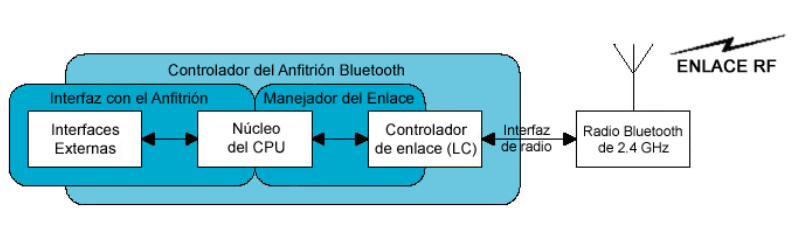
\includegraphics[width=15cm]{graphs/bluetooth_hardware.png}
	\caption{Arquitectura de Hardware del protocolo Bluetooth \cite{codificacion}}
	\label{figure:bluetoothhw} 
\end{figure}

El controlador digital esta compuesto por un CPU, por un procesador de señales digitales llamado Controlador de Enlace y por los interfaces con el dispositivo anfitrión. El controlador de enlace se encarga de hacer el procesamiento de la banda base y del manejo de los protocolos ARQ y FEC de la capa física para el manejo y corrección de errores. Además, se encarga de las funciones de transferencia (tanto asíncrona como síncrona), codificación de audio y encripción de datos. El CPU del dispositivo se encarga de atender las instrucciones relacionadas con Bluetooth del dispositivo anfitrión, para así simplificar su operación. Para ello, sobre el CPU corre un software denominado Manejador del Enlace, que tiene la función de comunicarse con otros dispositivos por medio del protocolo LMP.

\subsubsection{Arquitectura de Software}
Buscando ampliar la compatibilidad de los dispositivos Bluetooth, los dispositivos que se apegan al estándar utilizan como interfaz entre el dispositivo anfitrión (ordenador portátil, teléfono celular, etcétera) y el dispositivo Bluetooth como tal (chip Bluetooth) una interfaz denominada HCI (Host Controller Interface).

Los protocolos de alto nivel como el SDP (Protocolo utilizado para encontrar otros dispositivos Bluetooth dentro del rango de comunicación, encargado, también, de detectar la función de los dispositivos en rango), RFCOMM (Protocolo utilizado para emular conexiones de puerto serial) y TCS (Protocolo de control de telefonía) interactúan con el controlador de banda base a través del Protocolo L2CAP (Logical Link Control and Adaptation Protocol). El protocolo L2CAP se encarga de la segmentación y re-ensamblaje de los paquetes para poder enviar paquetes de mayor tamaño a través de la conexión Bluetooth. 

La arquitectura de software completa puede contemplarse en la figura \ref{figure:bluetoothsw}.

\begin{figure}[h] \centering
	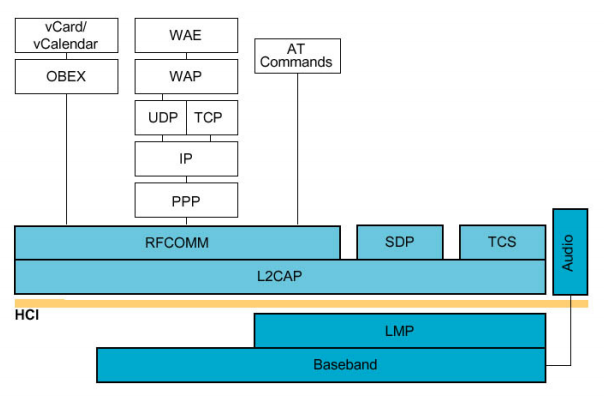
\includegraphics[width=15cm]{graphs/bluetooth_arquitectura_protocolos.png}
	\caption{Arquitectura de Software del protocolo Bluetooth \cite{codificacion}}
	\label{figure:bluetoothsw} 
\end{figure}

\subsection{Bluetooth de baja energía}

Bluetooth es uno de los protocolos inalámbricos más populares, y ha estado disponible en los teléfonos inteligentes, computadoras y otros dispositivos durante más de una década. El crecimiento explosivo de los dispositivos Bluetooth llevó a Bluetooth \ac{SIG} y a distintas empresas a la realización de que Bluetooth consumía demasiada energía y empleaba demasiado tiempo para conectarse en ciertas aplicaciones.

Bluetooth v4.0 introdujo \ac{BLE} , oficialmente conocido como \tit{Bluetooth Smart} o Bluetooth Inteligente. Esta especificación introduce un estándar radio completamente diferente, utilizando menos energía y con un coste menor, para así satisfacer las necesidades de estas nuevas aplicaciones. El amplio soporte de \ac{BLE} en teléfonos inteligentes y tabletas hace que las aplicaciones BLE sean fáciles de implementar y fáciles de usar para los consumidores.

El iPhone 4s de Apple introdujo soporte para \ac{BLE} y abrió el camino a un número masivo de dispositivos pequeños que son capaces de funcionar con pequeñas baterías. Antes de \ac{BLE}, el Bluetooth Clásico necesitaba baterías mas grandes por el gran uso de energía, y también requería de un chip de autentificación que era costoso. \ac{BLE} resuelve estos problemas para conectarse con iPhones y iPads. Muchos teléfonos basados en Android también presentan soporte para \ac{BLE}, concretamente desde la versión de Android 4.3. El \ac{SIG} de Bluetooth predice que para el 2018 más del 90 \% de los teléfonos móviles soportarán \ac{BLE}

Uno de los aspectos más poderosos de BLE es su flexibilidad y baja energía, que permite intercambiar información en forma genérica, a diferencia de la estructura rígida del Bluetooth Clásico.

\subsubsection{Comparación con otros protocolos}

Bluetooth y \ac{BLE} son protocolos que pueden simplificar la conectividad de productos, pero es importante entender como se comparan a otras tecnologías inalámbricas. WiFi, Zigbee y otros protocolos son mejores en ciertas aplicaciones  y \ac{BLE} no es siempre la mejor solución. La tabla \ref{table:blecomparison} muestra algunas de las características que diferencian a \ac{BLE} de ellos:

\begin{table}[H]%
	\centering
	\begin{tabular}{|c|c|c|c|}
		\hline
		\hline
		\tbf{}&\tbf{BLE} &\tbf{Wi-Fi}&\tbf{Zigbee}\\ \hline 
		\tbf{Banda de Frecuencia}&2.4 GHz&2.4 GHz / 5 GHz&2.4 GHz\\ \hline
		\tbf{Modulación}&GFSK&OFDM, DSSS&DSSS\\ \hline
		\tbf{Rango}&< 100m&< 300m&< 100m Punto a Punto\\ \hline
		\tbf{Topología de Red}&Scatternet&Star&Mesh\\ \hline
		\tbf{Velocidad}&1 Mbps&\specialcell{11 Mbps, 54 Mbps \\ 150 Mbps+}&250 kbps\\ \hline
		\tbf{Corriente Pico}&<15 mA&\specialcell{60 mA Rx \\ 200 mA Tx}&\specialcell{19mA Rx \\ 35mA Tx}\\ \hline
		\tbf{Corriente en Espera}&< 2 $\mu$A&< 100 $\mu$A&5 $\mu$A\\ \hline
		\hline 
	\end{tabular}
	\caption{Comparación de BLE con otros protocolos \cite{bluetoothlowenergy}}
	\label{table:blecomparison}
\end{table} 

Zigbee, Wi-Fi y \ac{BLE} utilizan la banda ISM de 2,4 GHz, pero son muy diferentes en sus capacidades. El transmisor \ac{BLE} es claramente un dispositivo de menor alcance que consume menos energía que Zigbee y especialmente Wi-Fi. El consumo de corriente pico más bajo es fundamental en el momento de elegir una batería. Wi-Fi, con un máximo de 200 mA nunca podría operar con una pila de botón. La corriente pico de \ac{BLE}, sin embargo, es mucho más baja.

A diferencia de Zigbee, \ac{BLE} no puede actualmente formar una red de malla, aunque si hay empresas que proveen de implementaciones específicas. Comunicación Punto a Punto implica que los dispositivos tienen que estar en el rango del teléfono inteligente para controlarlo. También hay soluciones utilizando una pasarela inalámbrica que conecta dispositivos \ac{BLE} a un enrutador, pero estos aumentan el coste final del producto.

\subsubsection{Capa física BLE}

\begin{figure}[h] \centering
	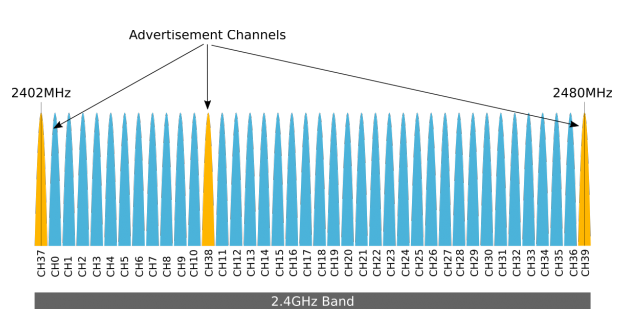
\includegraphics[width=15cm]{graphs/ble_capa_fisica.png} 
	\caption{Capa Física BLE \cite{bluetoothlowenergy}}
	\label{figure:capafisica}
\end{figure}

La capa física se relaciona directamente con la manera en la que los dispositivos \ac{BLE} transmiten y reciben datos.

\ac{BLE} utiliza la misma banda \ac{ISM} de 2,4 GHz que Bluetooth Clásico, abarcando desde 2400 MHz hasta 2483.5 MHz. Bluetooth v4.0 y especificaciones posteriores dividen la banda en 40 canales. Tal y como muestra la figura \ref{figure:capafisica}, 3 de estos canales son llamados “publicidad” y son utilizados por los dispositivos para enviar paquetes de publicidad con información sobre ellos para que otros dispositivos \ac{BLE} puedan conectarse. Estos canales se seleccionaron en la parte baja, media, y alta de la banda para evitar la interferencia de Wi-Fi. Por ejemplo, si el Canal 38 y canales cercanos están siendo interferidos por Wi-Fi, entonces todavía hay otros 2 canales de publicidad 37 y 39, que no se verán afectados y que \ac{BLE} puede usar.

\subsubsection{Capa de Enlace de Datos}
El verdadero funcionamiento de \ac{BLE} sucede en lo que se llama la capa de Enlace. Esta es la capa que tiene como funciones principales gestionar las conexiones y controlar los paquetes enviados y recibidos. Un dispositivo \ac{BLE} presenta varios estados posibles, aunque solo uno de ellos es permitido a la vez:

\begin{itemize}
\item Espera \\ El dispositivo no está transmitiendo o recibiendo, si no que está ``dormido'' para así ahorrar energía.
\item Publicidad \\ Un dispositivo que tiene un papel periférico entrará en el estado de publicidad, donde se enviarán paquetes en los canales de publicidad. En este estado también escuchará las respuestas a los paquetes desde un dispositivo central. Este modo es uno de los más críticos de entender desde una perspectiva de energía debido a que un dispositivo periférico pasará gran parte de su tiempo en el modo de Publicidad (dependiendo de la aplicación). El intervalo de Publicidad pues afecta directamente al consumo y duración de la batería.
\item Escaneo \\  Escaneo se refiere a escuchar los paquetes de publicidad que se envían a través de esos canales. Este modo se utiliza para buscar los dispositivos.
\item Iniciador \\ Este estado es el estado en el que un dispositivo central generalmente entra antes de establecer una conexión. El dispositivo central va a escuchar anuncios en los periféricos, pero una vez que el anuncio de la periférica deseada se recibe en el dispositivo, la central puede conectarse mediante el envío de los datos correctos.

Para el dispositivo esclavo, el estado Publicidad es también el estado inicial antes del estado de conexión. El estado de conexión es el estado final en el que el esclavo (periférico) y maestro (central) pueden intercambiar datos.
En \ac{BLE}, los datos se intercambian periódicamente sobre eventos de conexión.

Los datos se transmiten en los canales de datos, que son los 37 canales no utilizados para la publicidad. Ambos dispositivos se pondrán de acuerdo sobre los canales a usar y alternarán el envío de los datos, siguiendo las normas establecidas por la especificación.

Una aplicación típica \ac{BLE} implica un chip conectado a diversos sensores. Un usuario con un teléfono inteligente entra en el rango del dispositivo \ac{BLE}. El sensor con BLE transmite paquetes de publicidad y una vez que el teléfono recibe el anuncio del paquete, comenzará el proceso de conexión para obtener los datos de los sensores.

\end{itemize}

\FloatBarrier
\section{Android}
\label{sec:AndroidIntro}
    Android es un sistema operativo que en sus inicios fue concebido para dispositivos móviles con pantalla táctil. Sin embargo, ha evolucionado en una plataforma que actualmente también engloba relojes inteligentes, televisores, automóviles e incluso electrodomésticos.

\begin{figure}[h] \centering
    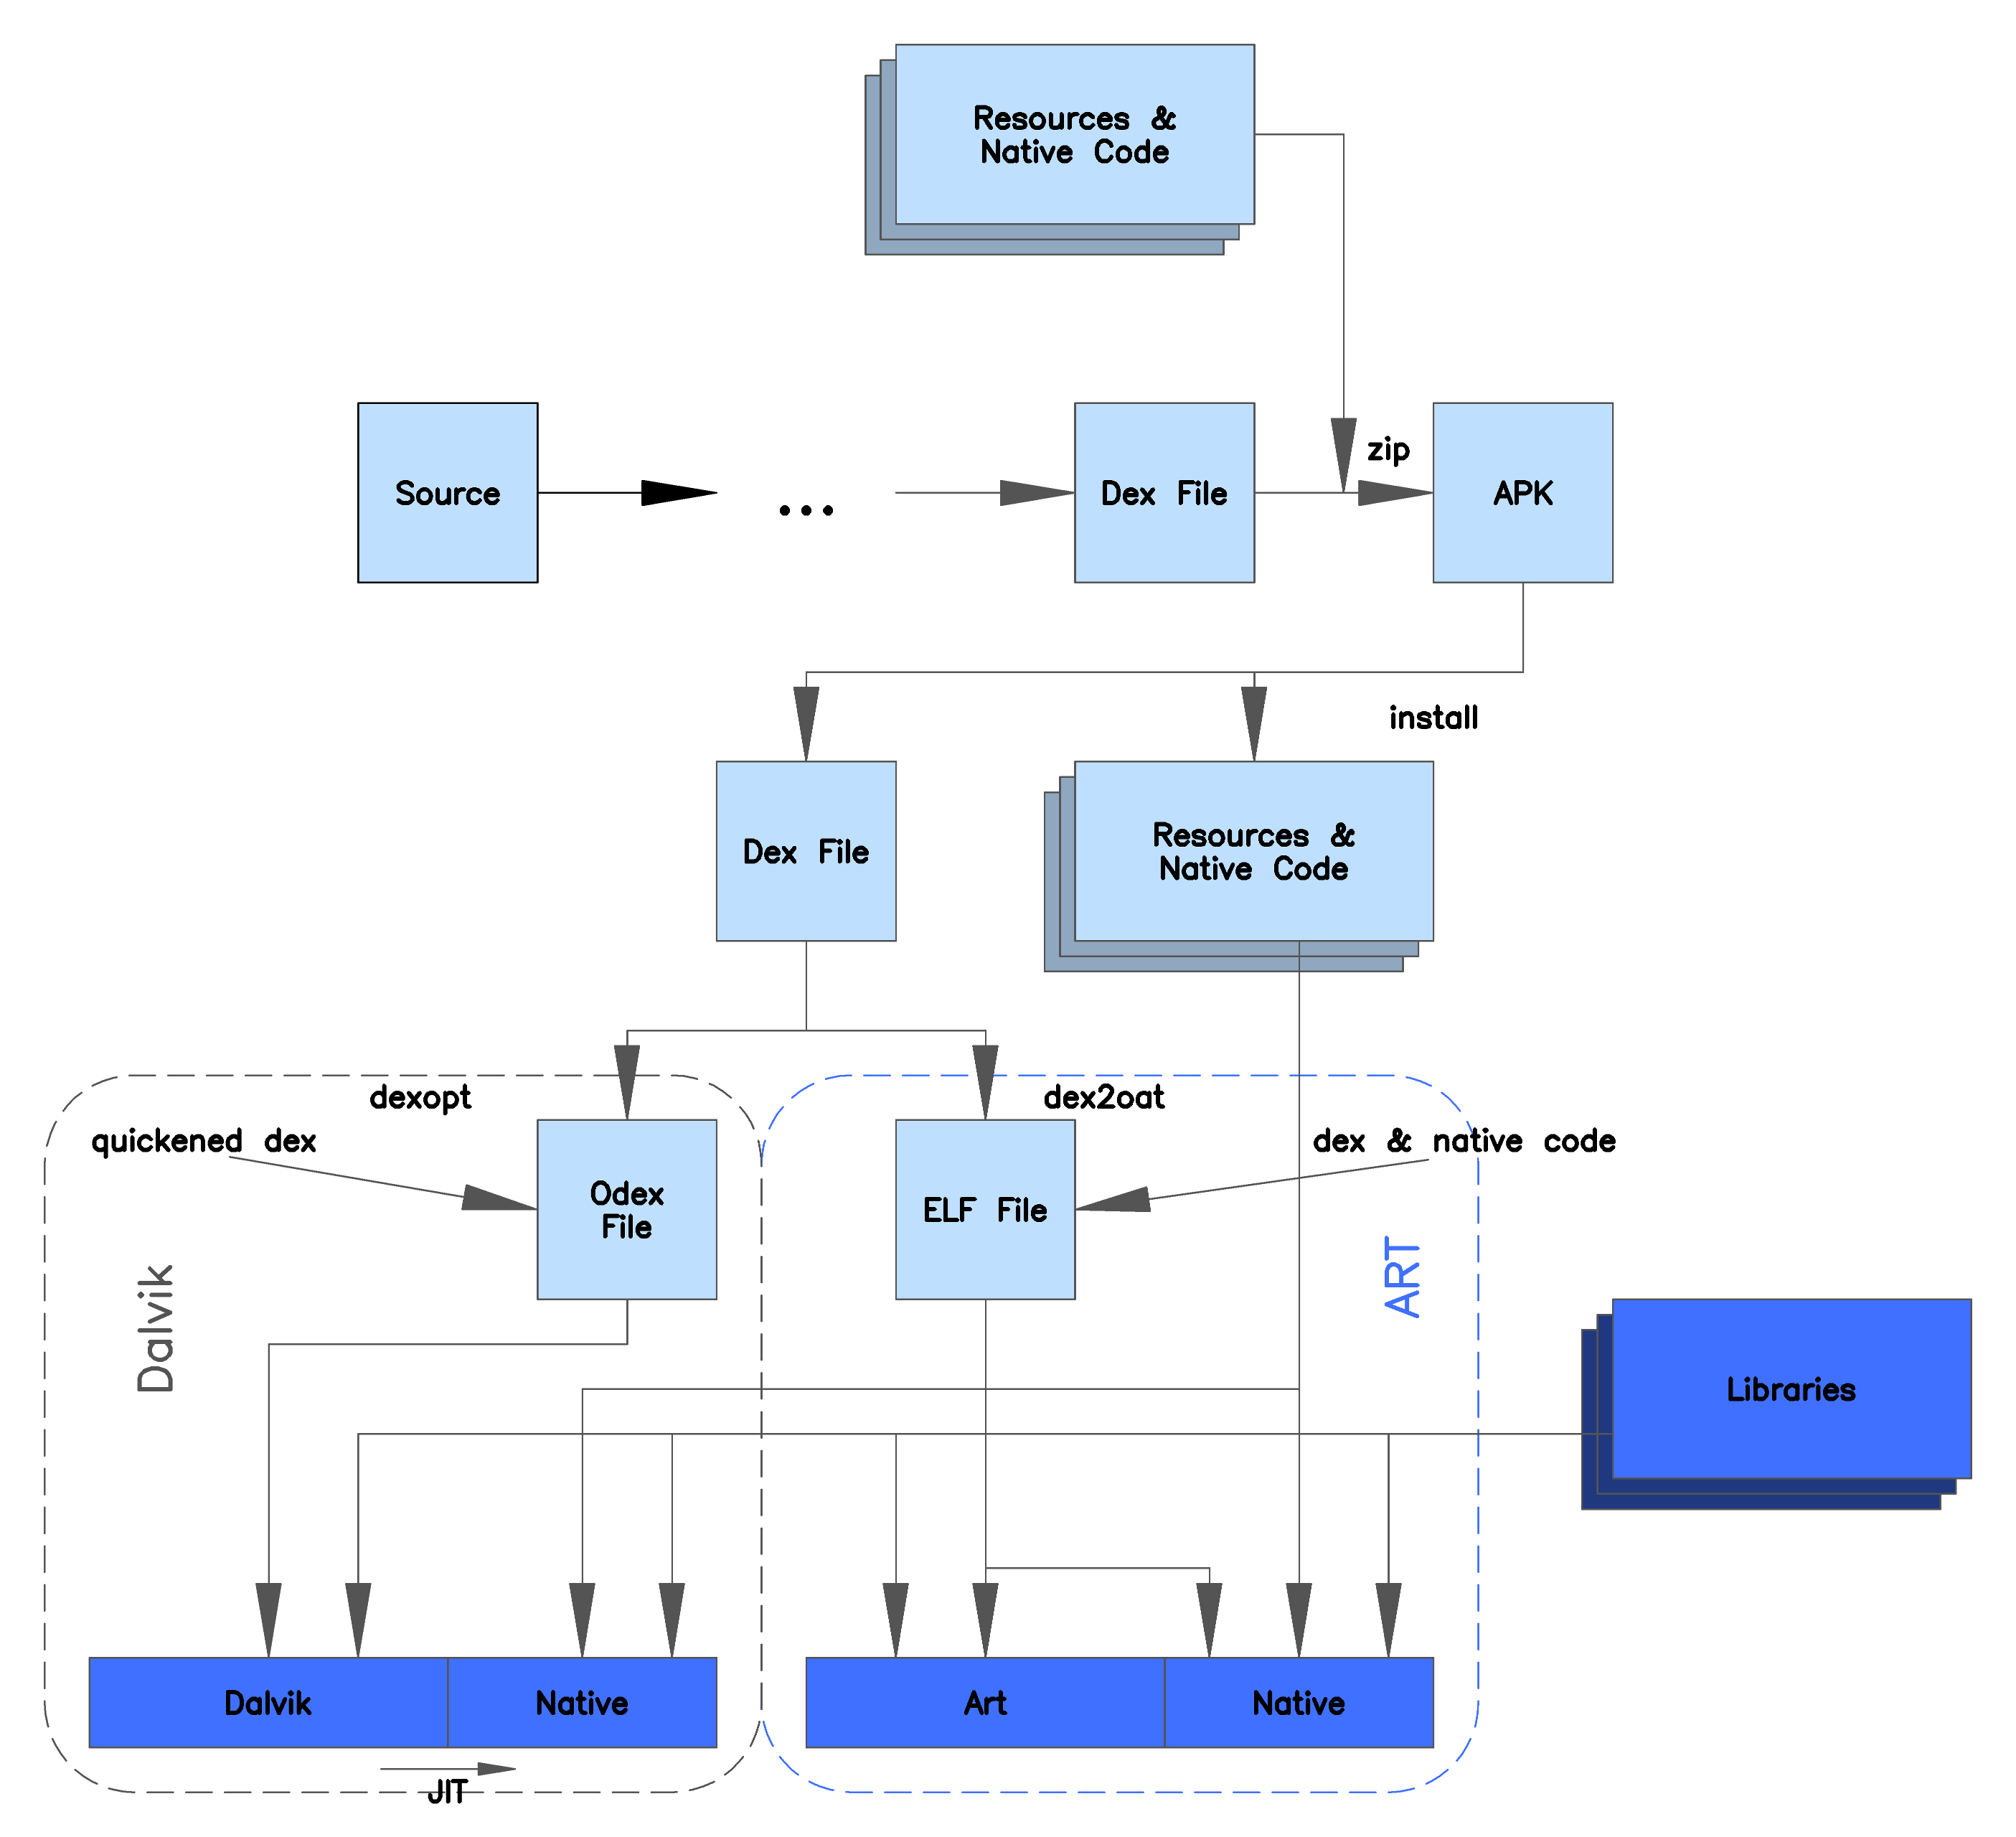
\includegraphics[height=12cm]{graphs/ART_view.png} \caption{Diagrama de la estructura del sistema operativo Android\cite{androiddevguide} }\label{fig:diagrama:ART}
\end{figure}

    Está basado en el núcleo de Linux. Sobre este, corre el entorno de ejecución propio de Android, que provee una máquina virtual (ya sea Dalvik o ART). Este a su vez ejecuta el código de las aplicaciones, escritas mayoritariamente en Java, aunque se permiten extensiones en C/C++. Las aplicaciones son precompiladas a un código intermedio denominado \ttw{Dex} y este es empaquetado y comprimido en el archivo estándar de aplicación Android, el \ttw{APK}. 

    Cada aplicación instalada en el dispositivo, es optimizada según los recursos y tipo de máquina virtual disponibles en el dispositivo en concreto. Al ser iniciada, es ejecutada dentro de un ``cajón de arena'', técnica que aísla los procesos de cada aplicación. Esto resulta en una mayor robustez y seguridad del sistema, ya que el fallo de una aplicación no afecta a los recursos de las demás. Tampoco podría una aplicación maligna, si se diera el caso, modificar o apropiarse de los recursos de otras. En la figura \ref{fig:diagrama:ART} se observa la relación entre todos los elementos anteriormente descritos.

\subsection{Interfaz}
    La interfaz de usuario por defecto de Android está basada en una manipulación directa, usando entrada táctil con gestos que vagamente corresponden a acciones físicas reales, tales como deslizar, golpear, pellizcar, etcétera. Para manipular objetos en pantalla. Además, la mayoría de dispositivos dispone de un teclado virtual, manipulado de la misma manera. 

    La respuesta del sistema a la entrada del usuario está diseñada para ser inmediata y dar una sensación de fluidez, utilizando las capacidades de vibración presentes en la mayoría de los dispositivos para proveer una respuesta háptica (no visual, no auditiva). Adicionalmente, algunas aplicaciones utilizan la información proveída por sensores tales como acelerómetros, giroscopios y sensores de proximidad para responder a interacciones adicionales, como por ejemplo ajustar la orientación de la pantalla cuando el dispositivo se encuentra apaisado o controlar alguna parte de la aplicación basándose en el azimut relativo del dispositivo.

\begin{figure}[h] \centering
    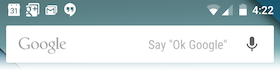
\includegraphics[width=8cm]{graphs/notification_area.png} \caption{Notificaciones minimizadas en el área de notificaciones\cite{androiddevguide} }\label{fig:screen:notification}
\end{figure}

    Una parte importante de la interfaz general de Android son las notificaciones, presentes en la barra de estado. Una notificación es un mensaje que una aplicación muestra al usuario fuera de los límites habituales de la interfaz de usuario de la aplicación. Las aplicaciones solicitan al sistema que emita una notificación por ellas, proveyendo el contenido, y el sistema operativo es quien maneja el resto del ciclo de vida de la notificación. En la figura \ref{fig:screen:notification} se pueden observar cuatro notificaciones minimizadas en el área de notificaciones

\subsection{Componentes de una aplicación}

\subsubsection{Contexto}
    Uno de los conceptos más importantes cuando se utiliza la plataforma Android es el contexto, \ttw{Context}. La clase \ttw{Context} en si misma no es más que una interfaz a información global acerca del entorno de una aplicación, y como tal es abstracta. Sin embargo, es importante ser consciente de qué elementos representan un contexto válido y qué elementos no. Un contexto permite acceso a recursos y clases específicos de la aplicación, y llamadas al sistema para operaciones a nivel de aplicación. Por ejemplo lanzar actividades, emitir mensajes de difusión o recibirlos.

\subsubsection{Actividades}
    En Android, una actividad (\ttw{Activity}) representa una única cosa concreta que el usuario puede realizar en la aplicación. La mayoría de las actividades interaccionan con el usuario, por tanto la clase \ttw{Activity} se encarga de crear una ventana donde se puedan insertar los componentes de la interfaz de usuario. Aunque las actividades suelen ser vistas por el usuario como ventanas a pantalla completa, también pueden ser usadas en otras múltiples maneras, ya sea como ventanas flotantes, o incrustadas dentro de otra actividad (mediante un \ttw{ActivityGroup})

\subsubsection{Ciclo de vida de una actividad}
    Las distintas actividades de las distintas aplicaciones instaladas en el dispositivo Android son gestionadas en forma de una ``pila de actividades''.
 
    Cuando el sistema Android se inicia, se presenta al usuario una pantalla principal, desde donde puede lanzar varias acciones y aplicaciones. A partir de ahí, cuando una nueva actividad es empezada, se emplaza arriba de la pila y se convierte en la actividad en ejecución. Las actividades previas, si las hubiera, siempre permanecen por debajo en la pila, y no se traerán al frente hasta que la nueva actividad finalice.

\begin{figure}[!htbp] \centering
    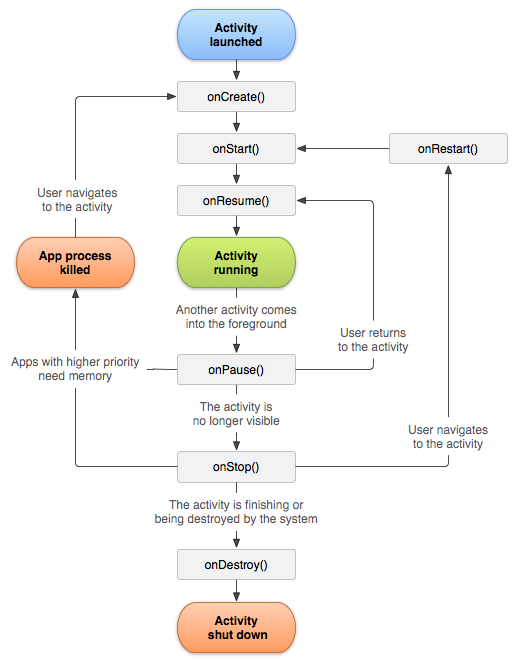
\includegraphics[width=12cm]{graphs/activity_lifecycle.png} \caption{Diagrama del ciclo de vida de una actividad en Android \cite{androiddevguide}.}\label{fig:diagrama:ActivityLifecycle}
\end{figure}

Una actividad tiene cuatro estados básicos:

\begin{description}
    \item[Activa] \hfill \\
     Una actividad está \tit{activa} cuando está presente en primer plano en la pantalla, es decir, arriba de la pila. También se puede decir que la actividad está \tit{En ejecución}.

    \item[Pausada] \hfill \\
    Si una actividad ha perdido el foco (ha dejado de estar en primer plano) pero todavía es visible, es decir, si una nueva actividad que no ocupa la totalidad de la pantalla o es transparente obtiene el primer plano, se encuentra \tit{pausada}. Una actividad pausada se conserva completamente íntegra (mantiene todos los estados y se mantiene suscrita al gestor de ventanas) pero puede ser matada por el sistema en condiciones extremas de baja memoria disponible.

    \item[Parada] \hfill \\
    Si una actividad se encuentra oculta por completo, el sistema la deja \tit{parada}. Mantiene estados e información de los miembros, pero sin embargo al no ser visible por el usuario es más probable que el sistema se deshaga de ella para liberar recursos cuando hagan falta.
    
    \item[Muerta] \hfill \\
    Cuando el sistema decide mover la actividad fuera de memoria, puede o bien finalizarla o matar el proceso. Cuando sea mostrada de nuevo al usuario, debe ser completamente reiniciada y restaurada a su estado previo.
\end{description}

    Los cuatro estados y las acciones que llevan a una aplicación de un estado a otro, junto con los métodos de la actividad que son invocados en cada etapa, están representados en la figura \ref{fig:diagrama:ActivityLifecycle}.

\FloatBarrier
\subsubsection{Servicios}
\label{ssec:teo:svc}

Un Servicio (\ttw{Service}) es un componente de la aplicación que puede realizar tareas de larga duración en segundo plano y no provee ninguna interfaz de usuario. Otro componente de la aplicación puede iniciar un servicio y este continuará en marcha en segundo plano, incluso si el usuario cambia a otra aplicación distinta. Además, un componente puede adherirse (\ttw{bind}) a un servicio para interactuar con él, e incluso realizar comunicación inter-procesos (IPC por sus siglas en inglés, Inter-Process Communication). Por ejemplo, un servicio puede manejar llamadas de red, reproducir música, realizar operaciones en el sistema de archivos, todo en segundo plano.

Un servicio puede tomar dos estados:

\begin{description}
    \item[Started] \hfill \\
    Un servicio está en estado \ttw{Started} (empezado) cuando un componente de la aplicación, por ejemplo una actividad, lo empieza llamando al método \ttw{startService()}. Una vez empezado de esta manera, un servicio puede continuar en segundo plano de manera indefinida, incluso si el componente que lo empezó ha sido destruido. Normalmente, suelen ser servicios que realizan una única operación y no devuelven ningún resultado. Por ejemplo, puede descargar o subir un archivo en la red. Cuando la operación ha sido completada, el servicio debe pararse a si mismo.
    
    \item[Bound] \hfill \\
    Un servicio está en estado \ttw{Bound} (adherido) cuando un componente de la aplicación se adhiere a él llamando al método \ttw{bindService()}. Un servicio adherido ofrece una interfaz servidor-cliente que permite a los componentes interaccionar con el servicio, mandar peticiones, obtener resultados, e incluso hacerlo entre distintos procesos mediante comunicación inter-proceso (IPC). Un servicio adherido solamente es activo durante el tiempo que otro componente esté adherido a él. Varios componentes pueden estar adheridos en un momento dado al servicio, pero cuando todos se desadhieren del servicio, el servicio es destruido.

\end{description}

\begin{figure}[h] \centering
    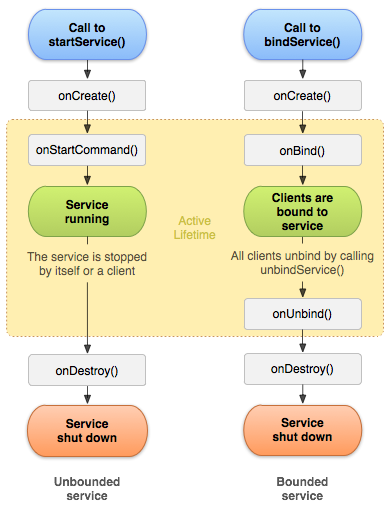
\includegraphics[width=9cm]{graphs/service_lifecycle.png} \caption{Diagrama del ciclo de vida de un servicio \cite{androiddevguide}}.\label{fig:diagrama:ServiceLifecycle}
\end{figure}

    Es necesario tener cuidado, dado que un servicio corre en el hilo principal de ejecución del proceso que lo llama, a no ser que se especifique lo contrario. Esto implica que, si el servicio va a realizar alguna tarea intensiva en CPU, o alguna operación bloqueadora, se debe de crear un nuevo hilo de ejecución dentro del servicio para ese propósito. De no hacerlo, se corre el riesgo de que la aplicación deje de responder y sea matada por el sistema operativo.

    Los dos tipos de ciclo de vida de un servicio, sus etapas y los métodos invocados en el transcurso de ellas están representados en la figura \ref{fig:diagrama:ServiceLifecycle}.

\FloatBarrier
\subsection{Vistas}
La interfaz gráfica de usuario en una aplicación Android está construida usando una jerarquía de vistas, objetos de la clase \ttw{View}, y grupos de vistas, objetos de la clase \ttw{ViewGroup}. Los objetos \ttw{View} suelen ser artilugios (widgets) de la interfaz de usuario, tales como botones o campos de texto, y los objetos \ttw{ViewGroup} son contenedores invisibles que definen cómo se posicionan las vistas que dependen de ellos, por ejemplo dispuestas en forma de rejilla o lista vertical.

Android provee un vocabulario XML que se corresponde con las subclases de \ttw{View} y \ttw{ViewGroup}, y permite definir la interfaz de usuario en XML usando una jerarquía de elementos de interfaz de usuario.

\subsection{Procesos e hilos de ejecución}
    En sistemas operativos, son básicos los conceptos de proceso e hilo de ejecución. En Android, el sistema operativo comienza un nuevo proceso Linux por cada primer componente de cada aplicación, con un único hilo de ejecución. Por defecto, todos los componentes de la misma aplicación corren en los mismos proceso e hilo de ejecución, el hilo principal de ejecución (\tit{main thread} en inglés). 

    En caso de que un componente de una aplicación sea inicializado, y ya exista un proceso para dicha aplicación en el sistema que otro componente de la misma aplicación ha inicializado, el nuevo componente se inicializa dentro del proceso original y usa el mismo hilo de ejecución. Sin embargo, se puede configurar una aplicación de manera que diferentes componentes corran en procesos separados, y siempre se pueden crear hilos de ejecución adicionales para cualquier proceso.

\subsubsection{Procesos}
    Como ya ha sido expuesto anteriormente, por defecto todos los componentes de la misma aplicación corren en el mismo proceso, y la mayoría de las aplicaciones no deberían de cambiarlo. Sin embargo, es posible controlar qué proceso pertenece a qué componente de ser necesario.

    El sistema operativo puede decidir apagar un proceso, cuando la cantidad de memoria disponible sea baja y haya requerimiento de ella por otro proceso que sirva de manera más inmediata al usuario. En este caso, los componentes dentro de dicho proceso que es apagado, son destruidos. Cuando estos componentes sean necesarios de nuevo, un nuevo proceso será comenzado por el sistema operativo para ello.

\subsubsection{Hilos de ejecución}
    Previamente se ha mencionado que todos los componentes de la misma aplicación corren en el mismo hilo de ejecución, el hilo principal de ejecución o \tit{main thread}. Este hilo es de suma importancia, dado que carga con la responsabilidad de despachar los eventos al widget de la interfaz de usuario que sea pertinente, incluyendo los eventos de dibujado en pantalla. Es también el hilo de ejecución en el que la aplicación interactúa con los componentes básicos de interfaz de usuario de Android, también conocidos como \tit{Android UI toolkit} (ubicados dentro de los paquetes java \ttw{android.widget} y \ttw{android.view}). Por todo esto, no es extraño encontrar denominado este hilo de ejecución como el hilo de la interfaz de usuario, o \tit{UI Thread}.

    Dado que todos los componentes que corren en el mismo proceso son instanciados en el hilo de ejecución principal, las llamadas del sistema operativo a cada componente son despachadas desde dicho hilo. En consecuencia, todos los métodos que responden a retrollamadas del sistema (\tit{system callbacks}), como por ejemplo para indicar que una tecla ha sido pulsada, siempre corren en el hilo principal de ejecución del proceso.

    Cuando el usuario toca un botón en la pantalla, el hilo principal de la aplicación despacha el evento de toque al widget pertinente, que reacciona cambiando su estado a presionado y manda una petición de invalidación a la cola de eventos. El hilo de ejecución principal entonces desencola la petición y notifica al widget que debe de re-dibujarse.

    Cuando una aplicación realiza trabajo intensivo en respuesta a una interacción del usuario, el modelo de hilo de ejecución único puede resultar en una falta de rendimiento. Concretamente, de suceder todo el procesamiento en el hilo principal de ejecución e iniciar tareas de larga ejecución tales como acceso a red o consultas a bases de datos, resultará en un bloqueo completo de la interfaz de usuario y su correspondiente hilo principal. Cuando el hilo de ejecución está bloqueado, no se pueden despachar eventos, eventos de dibujado en pantalla incluidos. Desde el punto de vista del usuario, esto se traduce en una aplicación que parece colgarse. En peores casos, en los que el hilo principal de ejecución está bloqueado por más de unos cuantos segundos (cinco segundos en la actualidad) el sistema operativo entrará en acción y mostrará una pantalla explicando que la aplicación ha dejado de responder, y matará la aplicación bloqueada. 

    Para evitar dicha penalización en el rendimiento, deben usarse hilos de ejecución alternativos para toda tarea que bloquee la ejecución o sea de alta carga procedural.

\FloatBarrier

\subsection{Ubicación}
\subsubsection{GPS}
El \ac{GPS} es un sistema de navegación por satélite que provee información sobre la posición y el reloj del dispositivo de recepción. El sistema fue desarrollado, instalado y empleado por el Departamento de Defensa de los Estados Unidos. Está constituido por 24 satélites en órbita geosíncrona y se basa en un sistema de triangulación para determinar posiciones con precisión de metros.

El funcionamiento del \ac{GPS} necesita la recepción de la señal de al menos cuatro de los 24 satélites en órbita. En base a dichas señales, que incluyen la identificación del satélite emisor y la hora de reloj de emisión, el aparato receptor sincroniza su reloj interno y calcula el tiempo que tardan en llegar las señales al equipo. Con dicha información, el dispositivo es capaz de conocer su distancia a cada uno de los satélites cuya señal es recibida, y por ende la posición absoluta del punto de medición.

\subsubsection{Servicios Móviles de Google}
Conocer la localización \ac{GPS} del dispositivo móvil es crítico en el funcionamiento de la aplicación. Es posible en un dispositivo Android utilizar el receptor \ac{GPS} a bajo nivel y recibir actualizaciones de posición en formato NMEA. Sin embargo, no se aprovecharían cantidad sustancial de optimizaciones que Google ofrece como parte de \ac{GMS} tales como tiempo de respuesta mejorado, localización mixta y consumo de batería mejorado. 

\ac{GMS} es un servicio en segundo plano propietario de Google presente en todos los dispositivos Android que satisfagan las condiciones de entrada de la empresa. En este proyecto, la aplicación se conectará a dicho servicio para requerir actualizaciones de posición.

\subsection{BLE en Android}
 Android 4.3 (Nivel API 18) introduce una función de soporte de la plataforma para Bluetooth de baja energía y proporciona una API que las aplicaciones pueden utilizar para detectar dispositivos \ac{BLE}, consultar servicios y realizar operaciones de lectura o escritura. En contraste con el Bluetooth clásico, \ac{BLE} está diseñado para proporcionar un consumo de energía significativamente menor. Esto permite que aplicaciones Android puedan comunicarse con dispositivos BLE que tienen requisitos de baja potencia, tales como sensores de proximidad, pulsómetros, sensores publicitarios y otros muchos más.
 
\subsubsection{Conceptos y Terminología clave}
A continuación presentamos un resumen de los conceptos y terminología que son de vital importancia cuando hablamos del protocolo BLE:
\begin{itemize}
\item \ac{GATT} \\ El \ac{GATT} es una especificación general para el envío y recepción de pequeñas cantidades de datos conocidos como ``atributos'' a través de un enlace BLE. Todos los perfiles actuales de aplicaciones de baja energía se basan en el GATT.
El SIG de Bluetooth define muchos perfiles para dispositivos de baja energía. Un perfil es una especificación para el funcionamiento de un dispositivo en una aplicación particular, teniendo en cuenta que un dispositivo puede aplicar más de un perfil. Por ejemplo, un dispositivo podría contener un monitor de ritmo cardíaco y un detector de nivel de batería.
\item \ac{ATT} \\ \ac{GATT} se define encima del protocolo \ac{ATT}. El conjunto también se conoce como el protocolo GATT/ATT. ATT está optimizado para funcionar en dispositivos BLE. Con este fin, se utiliza el menor número de bytes posible. Cada atributo está identificado por un identificador único universal (UUID), que es una cadena de caracteres representando un identificador con un formato de 128 bits normalizado, para así identificar de forma unívoca la información. Los atributos transportados por ATT reciben el nombre de características y servicios.
\item Característica \\ Una característica contiene un único valor y 0-n descriptores que describen el valor de dicha característica. Una característica puede ser interpretada como un tipo, análogo a una clase en \ac{POO}
\item Descriptor \\ Los descriptores son atributos definidos que describen el valor de una característica. Por ejemplo, un descriptor podría especificar una descripción legible por el ser humano, un rango aceptado para el valor de una característica, o una unidad de medida que es específica a un valor de una característica determinada.
\item Servicio \\ Un servicio es una colección de características. Por ejemplo, un usuario podría disponer de un servicio llamado \tit{Monitor de Frecuencia Cardíaca}, el cual incluye características tales como \tit{Medida del ritmo cardíaco} o \tit{Posición del dispositivo medidor en el cuerpo humano}, entre otras.
\end{itemize}

\subsubsection{Roles y Responsabilidades}
Los roles y responsabilidades aplicables cuando un dispositivo Android interactúa con un dispositivo BLE son los siguientes:
\begin{itemize}
\item Central vs. periférica. Esto se aplica a la propia conexión BLE. El dispositivo con el rol o papel central escanea, en busca de publicidad, y el dispositivo con el rol periférico realiza el anuncio.
\item Servidor GATT vs. cliente GATT. Esto determina cómo se realiza la comunicación entre los dos dispositivos una vez que la conexión ha sido establecida.
\end{itemize}

\begin{figure}[h] \centering
 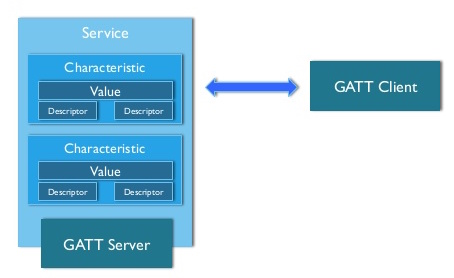
\includegraphics[height=7.5cm,keepaspectratio]{graphs/gattServerClient.png} \caption{Esquema Servidor y Cliente GATT \cite{androiddevguide}}\label{fig:gattconexion}
\end{figure}

Para entender la distinción, podemos imaginar que tenemos por un lado un teléfono Android y un rastreador de actividad como dispositivo BLE por otro. El teléfono es compatible con el papel central mientras que el rastreador de actividad se apoya en el papel periférico (para establecer una conexión BLE se necesitan dos dispositivos que presenten roles opuestos, ya que dos dispositivos que solo soporten modo periférico no podrían comunicarse entre sí, al igual que dos dispositivos que solo soportasen modo central).

Una vez que el teléfono y el rastreador de actividad han establecido una conexión, comienzan a transferir meta-datos GATT entre sí. Dependiendo del tipo de datos que se transfieren, el uno o el otro puede actuar como servidor. Por ejemplo, si el rastreador de actividad quiere reportar datos del sensor al teléfono, tendría sentido que el rastreador de actividad actuase como servidor. Si el rastreador de actividad quiere recibir actualizaciones desde el teléfono, entonces sería más conveniente designar al teléfono como el servidor, actuando el rastreador como cliente.

En nuestro caso particular, la aplicación Android (que se ejecuta en un dispositivo Android) es el cliente GATT. La aplicación recibe datos desde el servidor GATT, que es un pulsómetro comercial, el cual soporta el perfil BLE de ritmo cardíaco. La figura \ref{fig:gattconexion} muestra dicho esquema cliente-servidor.

\section{Desarrollo de aplicaciones web modernas}

\subsection{Definiciones básicas}

\subsubsection{Frontend}
El Frontend es un término muy utilizado en el desarrollo web actual, y podríamos resumirlo a que se refiere a la parte que el usuario común ve, es decir, la interfaz gráfica, aunque no se queda solo en eso, sino que dentro del Frontend podríamos decir que está el Javascript que se ejecuta del lado del cliente. Los lenguajes y tecnologías que componen el frontend son:

\begin{itemize}
\item \ac{HTML} \\ Define el contenido de una página web, como texto, imágenes y videos entre otros. Es un estándar a cargo de la W3C, organización dedicada a la estandarización de casi todas las tecnologías ligadas a la web, sobre todo en lo referente a su escritura e interpretación.
\item \ac{CSS} \\ Es un lenguaje usado para definir y crear la presentación de un documento estructurado escrito en HTML. La idea que se encuentra detrás del desarrollo de CSS es separar la estructura de un documento de su presentación.
\item Javascript \\ Es un lenguaje de programación interpretado, dialecto del estándar ECMAScript. Se define como orientado a objetos, basado en prototipos, imperativo, débilmente tipado y dinámico. En este caso nos referimos a Javascript del lado del cliente, implementado como parte de un navegador web, permitiendo mejoras en la interfaz de usuario y páginas web dinámicas.
\end{itemize}

\subsubsection{Backend}
Es lo que se ejecuta del lado del servidor. Los elementos del backend son los siguientes:

\begin{itemize}
\item Lógica de negocio.
\item Lenguaje de servidor (PHP, Ruby, Python, Javascript).
\item Bases de Datos
\end{itemize}

\subsubsection{Stack}
Un Stack, podríamos decir que es un conjunto de paquetes configurado de cierta manera que se complementan entre sí.
El ejemplo de un stack bastante conocido es LAMP, que es el conjunto de Linux, Apache, MySQL y PHP ejecutándose juntos como una plataforma para desarrollo web, o MEAN, el cual es bastante reciente y el usado en este proyecto, agrupando las tecnologías MongoDB, Express, AngularJS y Node.

\subsubsection{DOM}
\ac{DOM} es la estructura de objetos interna que genera el navegador cuando se carga un documento HTML y la cual se puede alterar mediante Javascript para cambiar de forma dinámica los contenidos y aspecto de la página. Es una estructura jerárquica donde existen varios objetos y unos dependen de otros.

Los objetos del DOM modelan tanto la ventana del navegador como el historial, el documento o página web, y todos los elementos que pueda tener dentro la propia página, como párrafos, divisiones, tablas, formularios y sus campos, etcétera. A través del DOM se puede acceder, por medio de Javascript, a cualquiera de estos elementos, es decir, a sus correspondientes objetos para alterar sus propiedades o invocar a sus métodos. Con todo, a través del DOM, queda disponible para los programadores de Javascript cualquier elemento de la página, para modificarlos, suprimirlos, crear nuevos elementos y colocarlos en la página, etcétera.

\subsubsection{Web Socket}
Especificación web que permite establecer una conexión persistente entre el cliente y el servidor, autorizando a ambas partes a enviar datos en cualquier momento.

\subsection{MEAN}
MEAN es un \tit{stack} para el desarrollo de aplicaciones web, el cual usa JavaScript como lenguaje de programación tanto para el frontend como para el backend, gracias a sus herramientas MongoDB, Express, AngularJS y NodeJS. Este es el motivo por el cual se denomina un \tit{full stack}. 
Podríamos considerarlo una alternativa a LAMP, aunque de cierta manera un poco lejana, ya que en LAMP utilizamos tecnologías distintas en cada cosa que queremos hacer.

\begin{table}[H]%
	\centering
	\begin{tabular}{|c|c|c|}
		\hline
		\hline
		\tbf{}&\tbf{LAMP/XAMPP} &\tbf{MEAN}\\ \hline 
		\tbf{Sistema Operativo}&\specialcell{Linux, Windows, \\ Mac OS X, etc...}&\specialcell{Linux, Windows, \\ Mac OS X, etc...}\\ \hline
		\tbf{Servidor HTTP}&Apache&Node.js\\ \hline
		\tbf{Base de Datos}&MySQL&MongoDB\\ \hline
		\tbf{Web Framework}&PHP&Express\\ \hline
		\tbf{Frontend Framework}&-&AngularJS\\ \hline
		\hline 
	\end{tabular}
	\caption{Comparación básica de LAMP y MEAN \cite{penflip}}
	\label{table:lampMean}
\end{table} 

\begin{table}[H]%
	\centering
	\begin{tabular}{|c|c|c|}
		\hline
		\hline
		\tbf{}&\tbf{LAMP} &\tbf{MEAN}\\ \hline 
		\tbf{Base}&Bash&Javascript\\ \hline
		\tbf{Servidor HTTP}&Apache Config&Javascript\\ \hline
		\tbf{Base de Datos}&SQL&Javascript\\ \hline
		\tbf{Lenguaje de Programación}&PHP&Javascript\\ \hline
		\hline 
	\end{tabular}
	\caption{Comparación entre lenguajes utilizados en LAMP y MEAN \cite{penflip}}
		\label{table:lampMeanLang}
\end{table} 

Como se puede observar en las tablas \ref{table:lampMean} y \ref{table:lampMeanLang} , lo único que comparten ambas pilas de desarrollo es la finalidad para la que se utilizan: desarrollo web. Otro de los puntos a revisar es el hecho de que LAMP no cuenta en sí con una librería JavaScript para el frontend, aunque podría usarse cualquier librería sin problema, como por ejemplo AngularJS o jQuery.

Por tanto, podemos decir que MEAN es un \tit{full stack} de desarrollo web con el que se pretende trabajar todo el tiempo con JavaScript. Este hecho se apoya en el gran progreso de optimización del lenguaje, llegando incluso a ser más rápido que otros lenguajes utilizados del lado del servidor, como PHP, Ruby y Python. 

A continuación vamos a analizar en detalle cada una de las herramientas y tecnologías que conforman el stack MEAN.

\subsection{MongoDB}
Sin duda alguna, MySQL es la base de datos más popular del mercado, aunque recientemente ha experimentado un bajón en su uso en favor de otros sistemas de gestión de bases de datos más abiertos, como MariaDB o PostgreSQL. Lo que tienen en común estos sistemas, es que son considerados ``Sistemas de Bases de Datos Relacionales'' y cumplen muy bien con su cometido, que es guardar información y recuperarla en cualquier momento con un alta disponibilidad. También tienen en común que para comunicarse con ellas necesitaremos dominar el lenguaje SQL.

El problema que presentan estas bases de datos son la velocidad de lectura cuando se tiene una gran demanda de datos y un crecimiento exponencial de la carga. Un ejemplo sencillo es el reflejado por las redes sociales, las cuales reciben miles de consultas por segundo que deben ser servidas de forma eficiente y siempre cuidando que, si hay algún error en uno de sus servidores, dicha información se encuentre disponible. 

Esta es una de las principales razones del nacimiento de las bases de datos NoSQL, que tal y como su nombre indica, no son bases de datos que se manejen con SQL y proveen una alta disponibilidad y eficiencia. Algunos ejemplos de estas bases de datos son MongoDB, HyperTable, Cassandra, CouchDB, etcétera.

Sin embargo, a pesar de que existen muchas alternativas de bases de datos NoSQL, podemos decir que pocas tienen la madurez, seguridad y velocidad necesarias para entrar en entornos de producción de alta exigencia. MongoDB es una de las pocas que puede hacer gala de ello, ya que presenta funciones bastante interesantes que la llevan a ser la base de datos favorita para muchas personas. A continuación destacamos los puntos clave:

\begin{itemize}
\item Desarrollada en C++ \\ C++ es un lenguaje de bajo nivel, lo que promete que alcanzará un gran rendimiento a la hora de exigirle. Los documentos son almacenados en estilo \ac{JSON}, por lo que no existen tablas, ni filas, ni columnas. Permite el uso de JavaScript para su manipulación.
\item Replicación \\ La base de datos incluye por defecto un sistema de replicación. Si introducimos un nuevo documento en nuestra base de datos, esta automáticamente lo replicará en otra base de datos en un servidor distinto. De esta manera nos aseguramos que nuestra información permanece segura y siempre disponible.
\item GridFS \\ Nos permite guardar documentos de cualquier tamaño sin afectar al rendimiento de la base de datos.
\end{itemize}

\subsection{Express}
Express es un framework de desarrollo de aplicaciones web minimalista y flexible para Node. Si bien la base sobre la que estaremos trabajando será Node, el sistema que nos ofrece por defecto para servir páginas es un poco complejo. Express nos abstrae de estas capas de bajo nivel, permitiéndonos crear un servidor web en muy pocos pasos.

Compite con rivales bastante fuertes en el mercado, como Meteor o Restify. Sin embargo, ninguno de ellos tiene la comunidad que Express tiene detrás brindando soporte. Prácticamente cualquier duda técnica que surja, podemos encontrar la solución en foros dedicados al soporte informático como StackOverflow o Quora. En cambio, otros frameworks, a pesar de ser muy buenos, no cuentan con esta ventaja.

Algunas de las características que Express nos ofrece son las siguientes:

\begin{itemize}
\item Sencillez
\item Comunidad bastante activa
\item Documentación de alta calidad
\item Compatibilidad con otros módulos
\item Alto Rendimiento, focalizándose en el enrutamiento
\end{itemize}

\subsection{AngularJS}
\label{angularJS}
AngularJS es un framework de JavaScript de código abierto, mantenido por Google, que ayuda con la gestión de lo que se conoce como aplicaciones de una sola página. Su objetivo es aumentar las aplicaciones basadas en navegador con capacidad de Modelo Vista Controlador (MVC), en un esfuerzo para hacer que el desarrollo y las pruebas sean más fáciles.

Algunas características que vienen acompañadas con AngularJS son:

\begin{itemize}
\item Comunidad \\ Al igual que Express, la comunidad es uno de sus puntos fuertes.
\item Herramientas \\  AngularJS proporciona numerosas herramientas que nos brindan facilidades con llamadas \ac{AJAX}, bucles, sistemas para clonado de objetos o arrays, sistema de monitorización de variables, etcétera.
\item Data-Binding \\ Se refiere a que, si desde el backend cambia de alguna manera el valor de una variable (y lo actualizamos en nuestro controlador), cambiará también en el frontend. Si en el frontend hay algún cambio, el valor de la variable automáticamente se actualizará sin tener que hacer llamadas extras para detectar dicho cambio. 
\item MVC \\ La forma en la que está estructurado AngularJS prácticamente nos obliga a tener nuestro código ordenado, utilizando controladores para mandar datos a la vista, además de modelos, directivas, servicios y filtros, entre otros.
\item Manejador de rutas \\ AngularJS incluye por defecto un manejador de rutas para implementar aplicaciones de una sola página, \tit{single page web applications}, es decir, compactar en una sola página todo el HTML y manejar toda la información mediante rutas y controladores, únicamente cargando lo que nos interesa y no toda la página. Con esto utilizamos menos recursos del servidor  y mejoramos el rendimiento desde el punto de vista del cliente con menos tiempo de carga y mejores respuestas.
\end{itemize}

Aunque profundizaremos a nivel técnico más adelante en el apartado \ref{Cliente}, se ha incluido en la figura \ref{ejemploAngular} un ejemplo sencillo de la sintaxis utilizada en AngularJS. Esta puede parecer un poco extraña al principio, pero que una vez que uno se acostumbra, es muy intuitiva y fácil de manejar.

\begin{figure}[h] \centering
	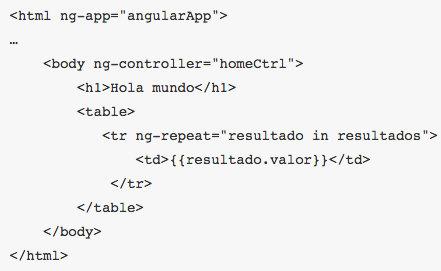
\includegraphics[height=7.5cm]{graphs/angular_example.png} \caption{Ejemplo de directivas AngularJS incrustadas en HTML \cite{penflip}}
	\label{ejemploAngular}
\end{figure}

\subsection{Node.js}
Node es un intérprete Javascript del lado del servidor que cambia la noción de cómo debería trabajar un servidor. Su meta es permitir a un programador construir aplicaciones altamente escalables y escribir código que maneje decenas de miles de conexiones simultáneas en una sola máquina física.

\subsubsection{¿Qué problema resuelve Node?}
La meta número uno declarada de Node es proporcionar una manera fácil para construir programas de red escalables. En lenguajes como Java y PHP, cada conexión genera un nuevo hilo que potencialmente viene acompañado de 2 MB de memoria. En un sistema de 8 GB de \ac{RAM}, el número teórico de conexiones concurrentes soportadas daría servicio como máximo a 4.000 usuarios al mismo tiempo. A medida que crece la base de clientes, si deseamos que nuestra aplicación soporte más usuarios, necesitaremos agregar más y más servidores.

Esto dispara el coste de servidor del negocio y el coste de tráfico, entre otros. Además de estos, están los costes causados por problemas técnicos potenciales. Por ejemplo, un usuario podría estar usando diferentes servidores para cada solicitud, así que cualquier recurso compartido debería almacenarse en todos los servidores. Por todas estas razones, el cuello de botella en toda la arquitectura de aplicación web (incluyendo el rendimiento del tráfico, la velocidad del procesador y la velocidad de la memoria) era el número máximo de conexiones concurrentes que podía manejar un servidor.

Node resuelve este problema cambiando la forma en que se realiza una conexión con el servidor. En lugar de generar un nuevo hilo en el sistema operativo para cada conexión (y de asignarle la memoria correspondiente), cada conexión dispara una ejecución de un evento dentro del proceso central del motor de Node. Node también asegura que nunca se quedará en punto muerto, puesto que no se permiten bloqueos y porque por naturaleza no se bloquea directamente para llamadas de entrada y salida. Con esto nos garantiza que un servidor que lo ejecute podrá soportar decenas de miles de conexiones concurrentes. La figura \ref{fig:nodeEvent} resume el sistema de eventos de Node.
\begin{figure}[h] \centering
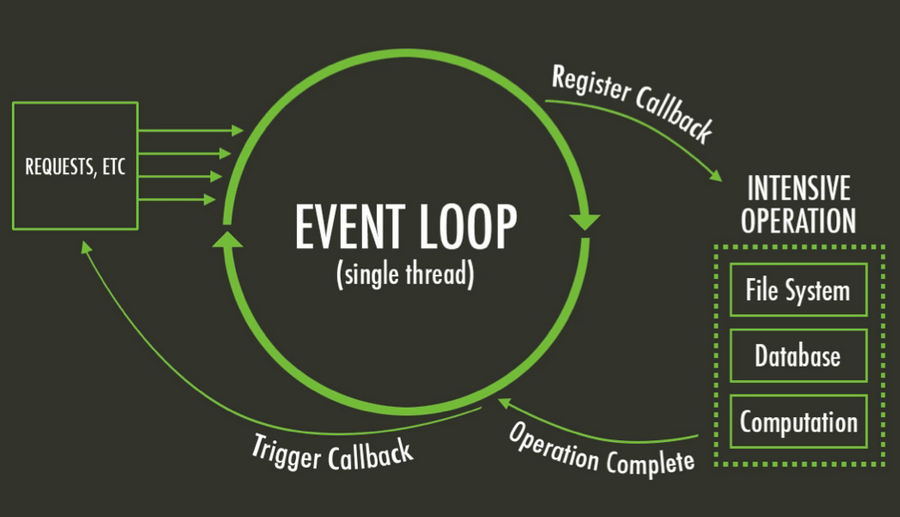
\includegraphics[width=15cm]{graphs/node_eventloop.png} \caption{Sistema de eventos en NodeJS \cite{nodejs}}
\label{fig:nodeEvent}
\end{figure}

\subsubsection{Funcionamiento}
Node ejecuta V8 JavaScript, es decir JavaScript del lado del servidor. El motor V8 JavaScript es el motor JavaScript subyacente que Google usa con su navegador Chrome. Un motor JavaScript interpreta el código y lo ejecuta. Con el V8, Google creó un intérprete ultra-rápido escrito en C++ con otro aspecto único: cualquiera puede descargar el motor e incorporarlo a cualquier aplicación que desee. Gracias a que este no está restringido a ejecutarse en un navegador, Node aprovechó está faceta y le dio otro propósito para así usarlo en el servidor.

\subsubsection{Programación orientada a eventos}
Node utiliza lo que se conoce como modelo de programación orientado por eventos, a diferencia de la programación orientada a objetos que utilizan lenguajes comúnmente usados como Java.
El lado del servidor realmente no es tan diferente del lado del cliente. Es cierto que el usuario no está interactuando con una página web en concreto, ya sea presionando botones o ingresando texto en campos, pero a un nivel superior, están sucediendo eventos. Ejemplos de estos pueden ser una conexión establecida, la recepción de datos a través de dicha conexión, o el hecho de dejar de recibir datos por esa conexión.
¿Por qué este tipo de configuración es ideal para Node? JavaScript es un gran lenguaje para la programación orientada a eventos, ya que permite funciones y cierres anónimos, y más importante, la sintaxis es similar para casi cualquier persona que haya programado en Java o C++. Las funciones de retrollamada o \tit{callbacks} que se llaman y ejecutan cuando ocurre un evento pueden escribirse en el mismo punto en el que el evento es capturado, con lo cual facilita la programación y el mantenimiento de estas. No existen arquitecturas complicadas orientadas a objetos ni tampoco interfaces, simplemente esperar por un evento y escribir una retrollamada qué contendrá las tareas a realizar cuando dicho evento ocurra.

\subsubsection{Módulos Node}
En NodeJS el código se organiza por medio de módulos, que son como los paquetes o librerías de otros lenguajes como Java. Por su parte, NPM es el nombre del gestor de paquetes que usamos en NodeJS.

NPM es bastante similar a los gestores de paquetes de Linux (apt-get en Ubuntu) y se puede entender como una forma de administrar módulos que deseamos tener instalados, distribuir los paquetes y agregar dependencias a nuestros programas.

El gestor de paquetes NPM, no obstante, difiere ligeramente de otros gestores de paquetes conocidos, ya que los instala localmente en los proyectos. Es decir, al descargarse un módulo, este se agrega a un proyecto local, que es el que lo tendrá disponible para incluir.

Cabe decir que también existe la posibilidad de instalar los paquetes de manera global en nuestro sistema, los cuales facilitan tareas relacionadas con el sistema operativo. Estos paquetes, una vez instalados, se convierten en comandos disponibles en el terminal, con los que se pueden realizar multitud de tareas. Ejemplos de este tipo de módulos son Bower, Grunt o Gulp.

\chapterend{}

% Capítulo 02.
%%%%%%%%%%%%%%%%%%%%%%%%%%%%%%%%%%%%%%%%%%%%%%%%%%%%%%%%%%%%%%%%%%%
%%% Documento LaTeX 																						%%%
%%%%%%%%%%%%%%%%%%%%%%%%%%%%%%%%%%%%%%%%%%%%%%%%%%%%%%%%%%%%%%%%%%%
% Título:		Capítulo 2
% Autor:  	Ignacio Moreno Doblas
% Fecha:  	2014-02-01
% Versión:	0.5.0
%%%%%%%%%%%%%%%%%%%%%%%%%%%%%%%%%%%%%%%%%%%%%%%%%%%%%%%%%%%%%%%%%%%
\chapterbegin{Implementación}
\label{chp:Impl}
%\minitoc

\section{Análisis de requisitos}
\label{sec:Requirements}

Para el desarrollo de este proyecto se han tenido en cuenta una serie de requisitos previos mínimos, necesarios para una correcta implementación del mismo. Los requisitos funcionales del sistema pueden ser divididos en 2 categorías, dependiendo si nos referimos a la aplicación Android o Web, y fueron acordados en los siguientes:

\subsection{Requisitos funcionales}

\subsubsection{Aplicación Android}

\begin{itemize}
	
\item Capacidad de detectar sensores \ac{BLE} próximos al dispositivo

La aplicación Android debe ser capaz de escanear y detectar cualquier sensor BLE que se encuentre dentro del radio de alcance del dispositivo Android, mostrando su nombre y dirección \ac{MAC} en pantalla.

\item Capacidad de conectarse a cualquier sensor BLE registrado.

La aplicación Android debe ser capaz de establecer una conexión GATT cliente-servidor, mostrando en pantalla los servicios y características ofrecidas por el sensor.

\item Capacidad de leer características GATT ofrecidas por el sensor.

La aplicación Android debe ser capaz de interpretar la información proporcionada por un sensor de ritmo cardíaco o pulsómetro comercial, pudiendo determinar entre otros, la frecuencia cardíaca del usuario o el porcentaje de batería restante.

\item Capacidad de determinar la posición del dispositivo

La aplicación Android debe de ser capaz de determinar la posición geográfica del dispositivo, en términos de latitud y longitud.

\item Capacidad de enviar los parámetros relevantes a través del protocolo HTTP a nuestro servidor web.

La aplicación Android debe ser capaz de enviar valores de frecuencia cardíaca y  localización al servidor web implementado, a través de solicitudes tipo POST del protocolo HTTP.

\end{itemize}

\subsubsection{Aplicación Web}

\begin{itemize}
	
\item Capacidad de determinar si el pulsómetro está conectado al sistema

La aplicación Web deberá reflejar en todo momento si el pulsómetro se encuentra conectado al sistema y emitiendo datos, o si este se encuentra desconectado.

\item Capacidad de mostrar la frecuencia cardíaca actual en tiempo real

El servidor web permanecerá a la escucha de peticiones POST efectuadas por la aplicación puente Android. Estas peticiones contendrán el último valor leído de frecuencia cardíaca y serán inmediatamente transmitidas al cliente web (cualquier navegador) a través de una conexión web socket. El navegador por tanto mostrará en pantalla el último valor recibido mediante una etiqueta numérica.

\item Capacidad de mostrar la evolución de la frecuencia cardíaca mediante el uso de una gráfica dinámica

La aplicación web será capaz de retener un cierto número de valores pasados (dependiendo del tamaño de la pantalla en al cual realizamos la visualización), junto con el valor actual y mostrará dichos valores en una gráfica lineal, la cual dará la sensación de avanzar en el tiempo conforme nuevos valores llegan al cliente web a través de la conexión web socket.

\item Capacidad de guardar los datos de frecuencia cardíaca en una base de datos

El servidor web implementado almacenará cada valor recibido en una base de datos no relacional, reflejando la fecha exacta en la cual tuvo lugar dicha muestra. Esto facilita la futura consulta de valores en ciertos rangos de tiempo para así permitir la posible realización de gráficas y estadísticas a tal efecto.

\item Capacidad de determinar la posición del usuario usando el servicio de mapas de Google

La aplicación web debe ser capaz de mostrar en todo momento la localización del usuario haciendo uso del pulsómetro.

\item Capacidad de notificar por e-mail a un grupo de usuarios interesados en realizar tareas de monitorización

Cuando el valor de ritmo cardíaco sobrepase un cierto rango, se enviará una notificación por e-mail alertando de condiciones anormales, junto con la localización actual del usuario usando el pulsómetro y se mantendrá al interesado o grupo de interesados informado con actualizaciones frecuentes, hasta la que la situación vuelva a la normalidad.

\item Capacidad de adaptarse fácilmente a pantallas más pequeñas, tales como teléfonos móviles y tabletas

La aplicación debe ser \tit{web responsive} y amigable para el usuario en cualquier tipo de pantalla.
 
\end{itemize}

\subsection{Requisitos no funcionales}

Adicionalmente, los siguientes requisitos no funcionales fueron considerados, refiriéndose a la Aplicación como el conjunto Android + Web.

\begin{itemize}
\item Extensibilidad futura.
La aplicación debe de ser fácilmente extensible en un futuro. Para ello se tendrá en mente la modularidad y el código autoexplicativo durante el desarrollo de la aplicación 

\item Tolerancia a fallos.
La aplicación debe de tolerar pequeños fallos sin que estos entorpezcan en medida alguna la posible medición en curso.

\item Rendimiento.
La aplicación no debe de ser una carga importante para el rendimiento del sistema, ya que esto podría resultar en mediciones imprecisas o pérdida de muestras por incapacidad del sistema de copar con la carga.

\item Usabilidad.
La aplicación no debe presentar un dificultoso manejo de cara al usuario.

\end{itemize}

\subsection{Diseño de la interfaz gráfica}

Como paso previo a la implementación en código, se han diseñado unos borradores de las distintas pantallas de las que constará la aplicación, tanto web como Android.

\subsubsection{Android}
La aplicación se ha dividido en cuatro pantallas básicas: reposo, búsqueda, desconectado y conectado, las cuales se pueden observar en las figuras \ref{fig:mockup:reposo}, \ref{fig:mockup:busqueda},  \ref{fig:mockup:desconectado} y \ref{fig:mockup:conectado} respectivamente:

\begin{figure}[h] \centering
\begin{minipage}{0.45\textwidth}\centering
 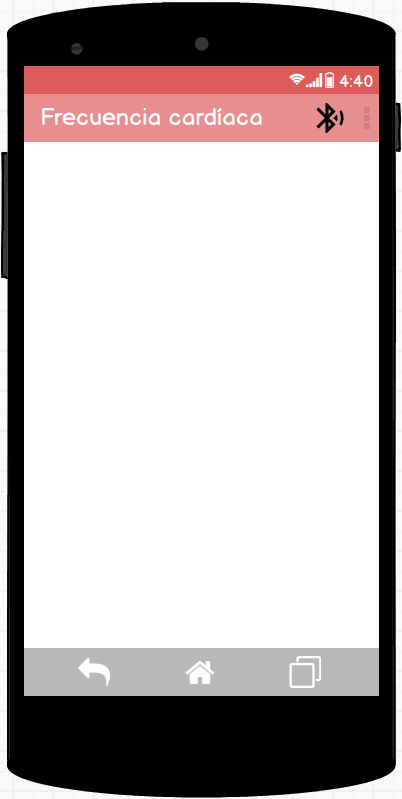
\includegraphics[height=12cm]{graphs/mockup_android_initial_es.png} \caption{Bosquejo Android estado Reposo}\label{fig:mockup:reposo}
\end{minipage}\hfill
\begin{minipage}{0.45\textwidth}\centering
   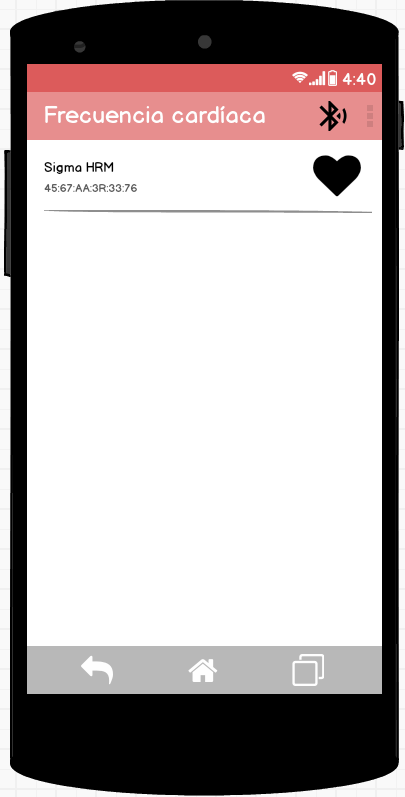
\includegraphics[height=12cm]{graphs/mockup_android_searching_es.png} \caption{Bosquejo Android estado Búsqueda}\label{fig:mockup:busqueda}
 \end{minipage}
\end{figure}

\begin{figure}[h] \centering
	\begin{minipage}{0.45\textwidth}\centering
		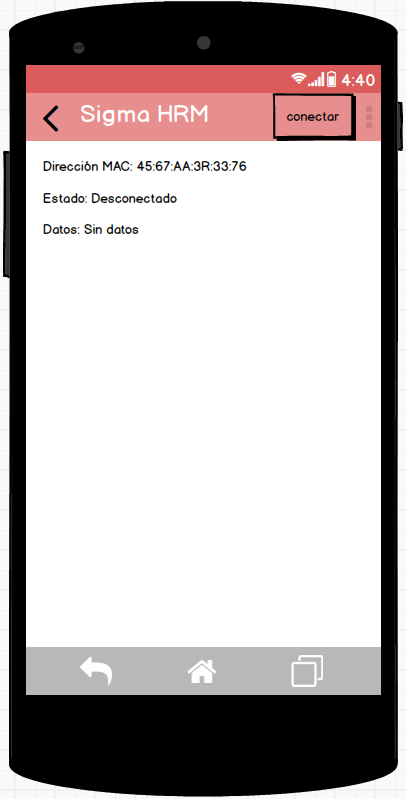
\includegraphics[height=12cm]{graphs/mockup_android_device_es.png} \caption{Bosquejo Android estado Desconectado}\label{fig:mockup:desconectado}
	\end{minipage}\hfill
	\begin{minipage}{0.45\textwidth}\centering
		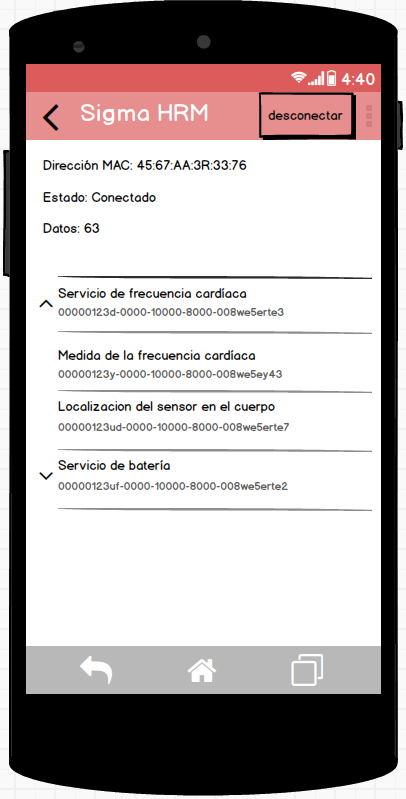
\includegraphics[height=12cm]{graphs/mockup_android_emitiendo_es.png} \caption{Bosquejo Android estado Conectado}\label{fig:mockup:conectado}
	\end{minipage}
\end{figure}

\begin{description}
\item Reposo\hfill \\
Representa la primera actividad que será cargada en primer plano cuando lancemos la aplicación. Para empezar a escanear dispositivos dentro del alcance de nuestro teléfono debemos pulsar el botón situado en la barra de acción superior, cuyo icono es el logotipo de Bluetooth.
\item Búsqueda\hfill \\
Muestra una lista con los dispositivos sensores BLE encontrados, en particular el nombre y dirección \ac{MAC} del dispositivo. Para obtener información de cualquiera de los sensores, debemos pulsar el elemento correspondiente en la lista. Esto nos llevará a la actividad de perfil del dispositivo, en principio en su estado \tit{desconectado}.
\item Desconectado\hfill \\
 Muestra una interfaz gráfica básica para la monitorización de la conexión, junto con la dirección \ac{MAC} del sensor. Para conectarnos al dispositivo debemos pulsar en el botón conectar situado en la barra de acción superior. Una vez que la conexión Bluetooth ha sido establecida, la interfaz de usuario cambiará a su estado \tit{conectado}.
\item Conectado\hfill \\
 Muestra una lista expandible de los servicios ofrecidos por el sensor. Para consultar las características que un servicio en particular contiene, debemos pulsar en dicho elemento de la lista y esto hará que se expandan las características disponibles. Para empezar a recibir datos del sensor debemos pulsar en cualquier característica, lo que actualizará el campo ``datos'' de la actividad mostrando el valor recibido. Mediante el pulsado de la característica ``Medida de la Frecuencia Cardíaca'' activaremos e instanciaremos el cliente HTTP para así comenzar a enviar valores de ritmo cardíaco en tiempo real y la localización geográfica del usuario a nuestro servidor web mediante solicitudes de tipo POST y la aplicación podrá seguir funcionando en segundo plano, hasta que decidamos desconectar.
\end{description} 

\subsubsection{Web}
La aplicación web presenta dos estados básicos en cuanto a la interfaz gráfica se refiere, que son desconectado y conectado,  las cuales pueden contemplarse en las figuras \ref{fig:mockup:web:desconectado} y \ref{fig:mockup:web:conectado} respectivamente. Si la aplicación Android se encuentra en estado \tit{conectado}, la aplicación web automáticamente se encontrará en estado \tit{conectado} mostrando una gráfica con los últimos valores recibidos junto con el valor actual. El resto de posibles estados de la aplicación Android se corresponderán con el estado \tit{desconectado} de la aplicación web.

\begin{figure}[h] \centering
	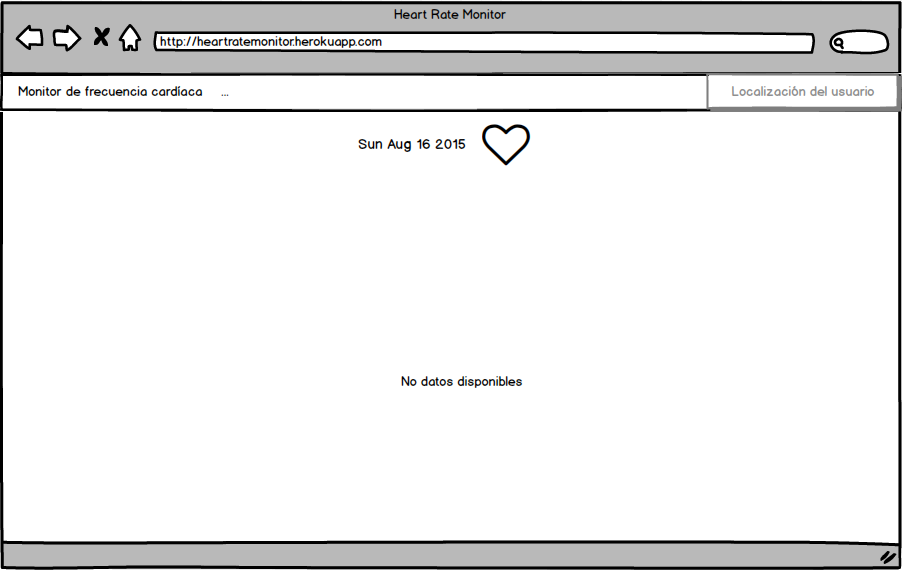
\includegraphics[width=15cm]{graphs/mockup_web_disconnected_es.png} \caption{Bosquejo web con sensor desconectado}\label{fig:mockup:web:desconectado}
\end{figure}

\begin{figure}[h] \centering
	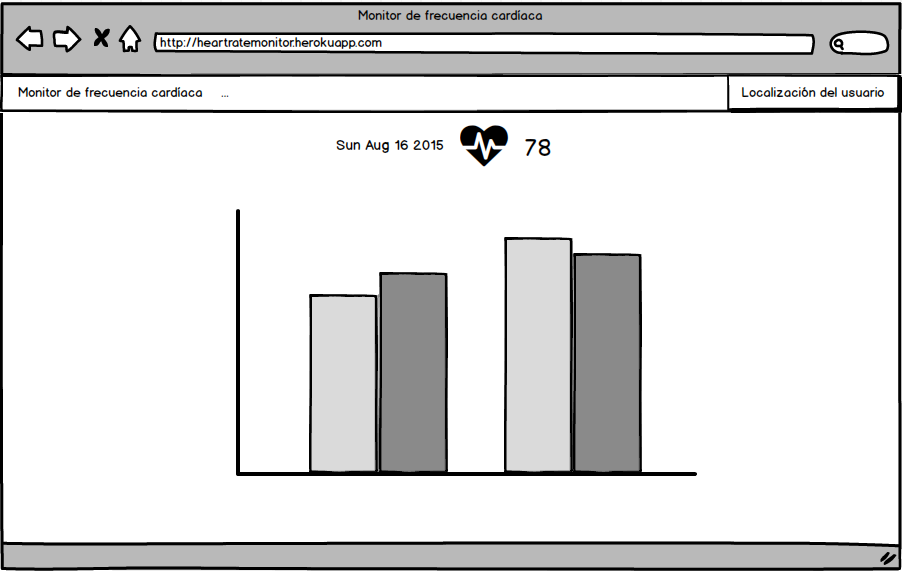
\includegraphics[width=15cm]{graphs/mockup_web_connected_es.png} \caption{Bosquejo web con sensor conectado}\label{fig:mockup:web:conectado}
\end{figure}

El botón con etiqueta ``Localización del usuario''  nos redirigirá al servicio de mapas de Google mostrando la localización del poseedor del sensor en ese preciso instante y estará habilitado unicamente si nos encontramos en el estado \tit{conectado}.


\subsection{Dispositivo Android}
    El desarrollo de este proyecto ha sido realizado y probado en un Google Nexus 5, bajo la versión Android 5.0, lo cual garantiza que la aplicación conserva toda su funcionalidad en los modelos más modernos, tanto en software como en hardware. 
    
    La versión mínima de Android requerida para el correcto funcionamiento de esta aplicación, es el nivel de \ac{API} 18, correspondiente a Android 4.3, ya que es la primera versión que incorpora soporte para BLE.

\section{Aplicación Android}

\subsection{Entorno de desarrollo integrado}
\label{sec:IDE}
\begin{figure}[h] \centering
    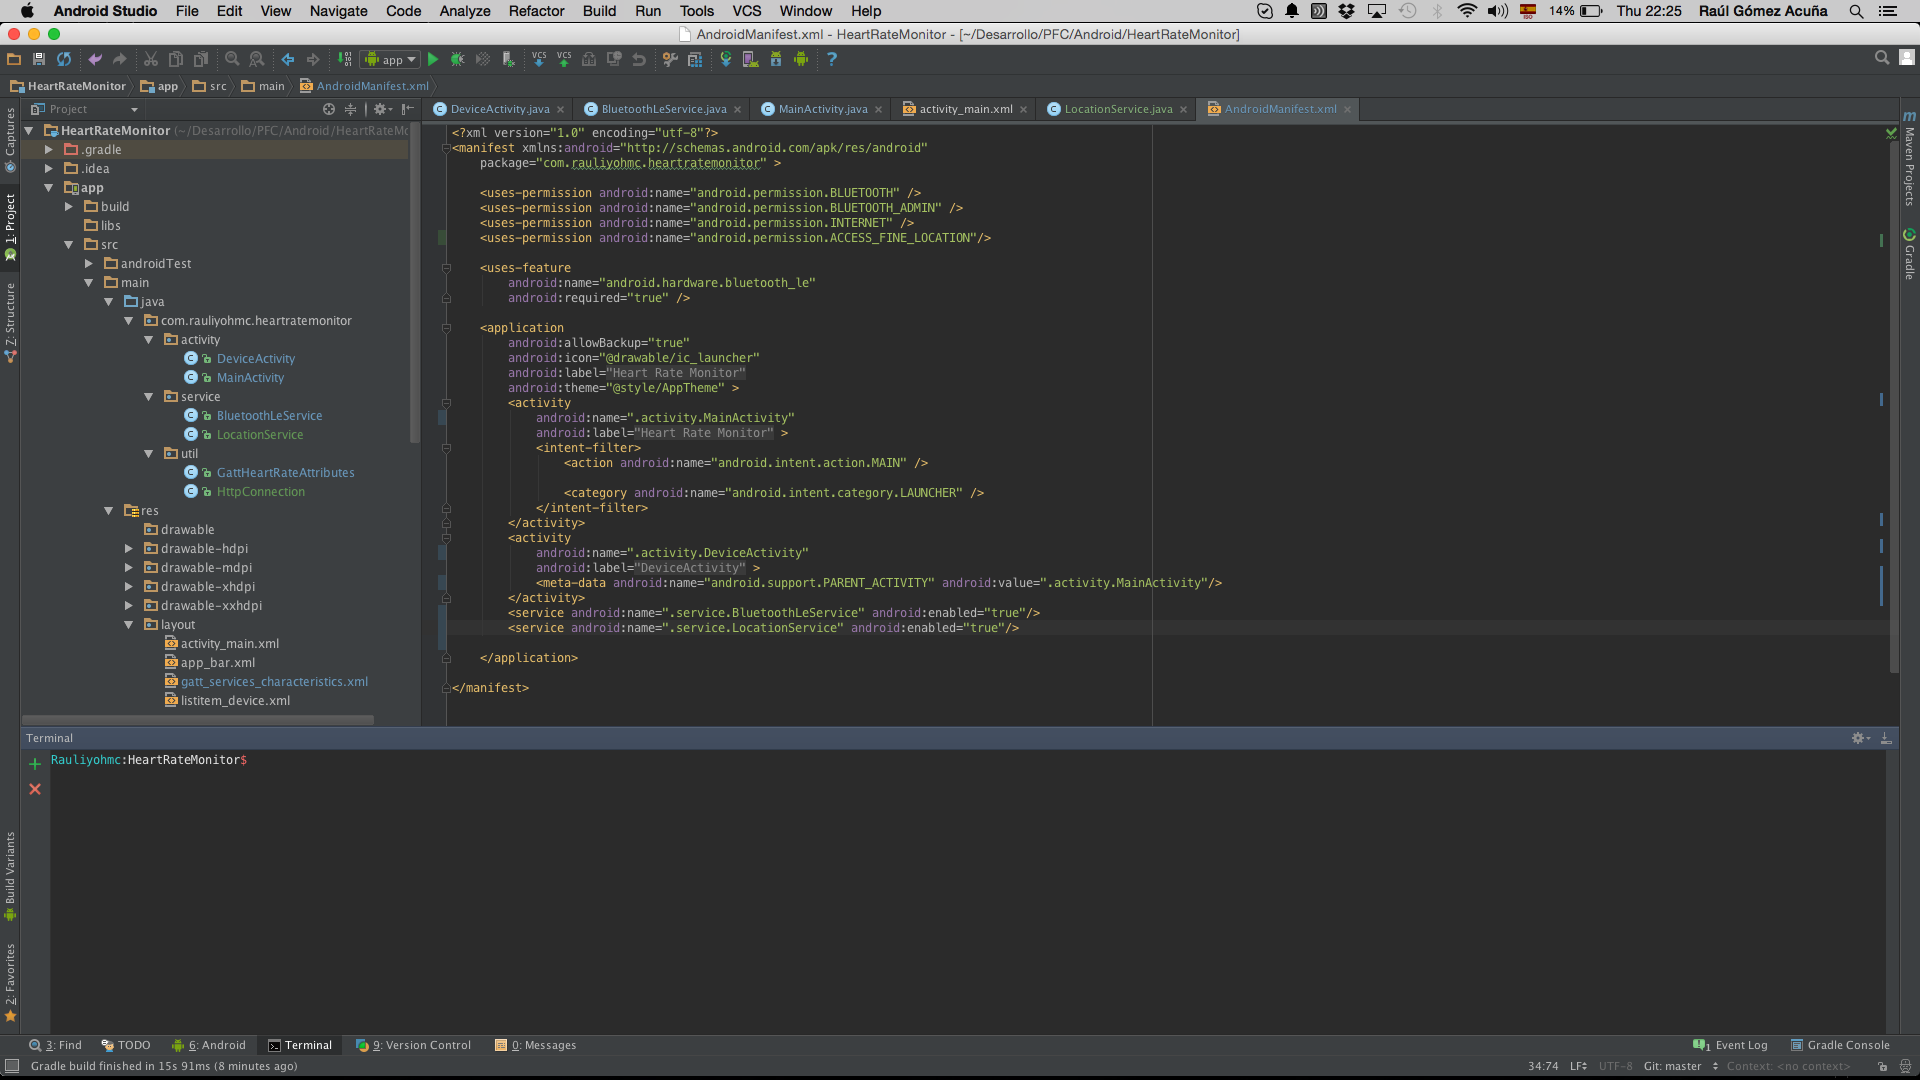
\includegraphics[width=15cm]{graphs/android_studio.png} \caption{Entorno de desarrollo integrado Android Studio}\label{fig:astudio}
\end{figure}
 \begin{figure}[h] \centering
    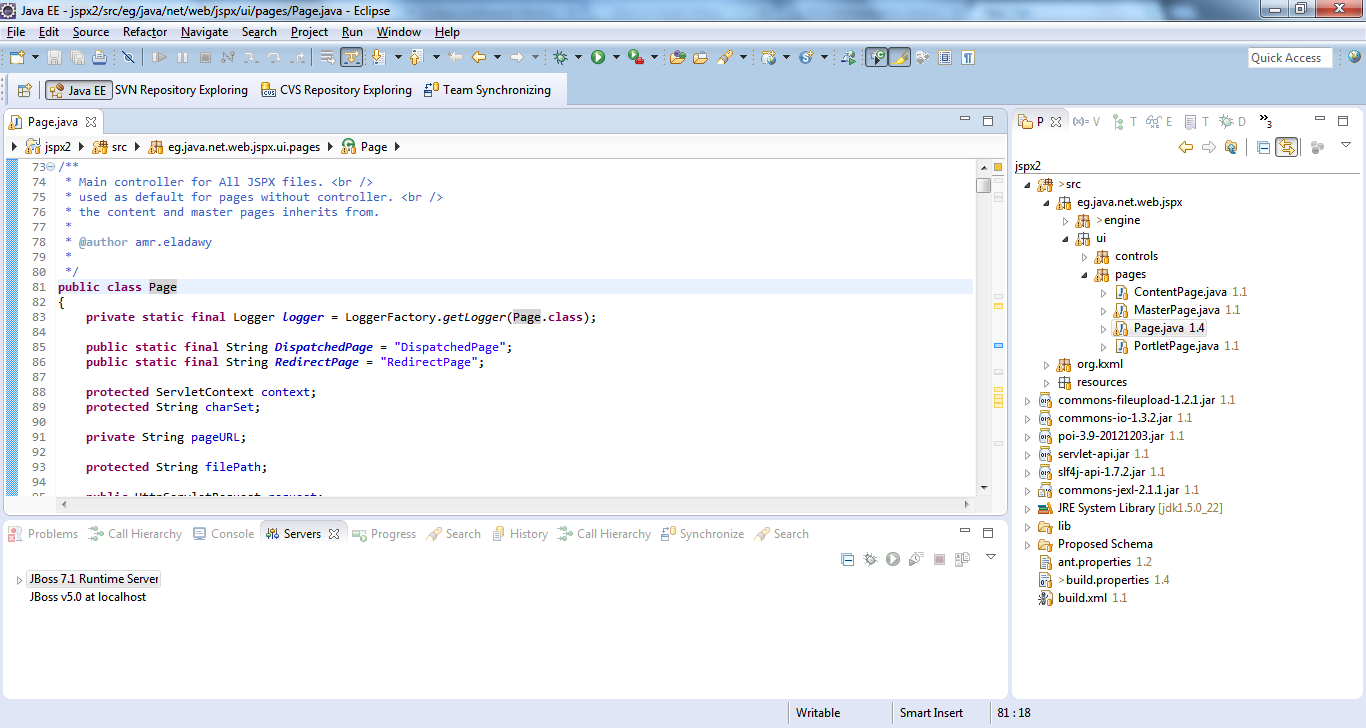
\includegraphics[width=15cm]{graphs/eclipse.png} \caption{Entorno de desarrollo integrado Eclipse}\label{fig:eclipse}
\end{figure}
    Es posible elegir entre varios entornos integrados de desarrollo a la hora de desarrollar una aplicación para la plataforma Android. Los dos principales son Eclipse y Android Studio.
    
    Android Studio es un \ac{IDE} específico para desarrollar en la plataforma Android. Está basado en el popular IntelliJ IDEA de la compañía JetBrains, pero fuertemente modificado, tanto en aspecto como en funcionalidad. Android Studio es de reciente desarrollo, llegando a su versión 1.0 inicial en Diciembre de 2014. La versión 1.0.2 se puede observar en la figura \ref{fig:astudio}.

    Eclipse es un \ac{IDE} de propósito general, que provee un espacio de trabajo y un sistema de complementos muy extensible y flexible. Está escrito en Java, e inicialmente se enfocó al desarrollo en dicho lenguaje. 
    
    Gracias a su sistema de complementos, Eclipse puede ser utilizado para desarrollar aplicaciones en múltiples lenguajes: Ada, ABAP, C, C++, COBOL, Fortran, Haskell, JavaScript, Lasso, Lua, Natural, Perl, PHP, Prolog, Python, R, Ruby (inlcuyendo el framework Ruby on Rails), Scala, Clojure, Groovy, Scheme y Erlang. Eclipse fue también el primer \ac{IDE} con soporte para desarrollo en la plataforma Android. La figura \ref{fig:eclipse} muestra la versión 4.4 Luna.

    A la hora de realizar el proyecto, se consideraron ambas soluciones, y se optó por utlizar el entorno de desarrollo integrado Android Studio, por varias razones.
\begin{itemize}
\item Android Studio utiliza Gradle como su sistema de compilación, el cual resulta mucho más claro y menos tedioso de lidiar que ANT, el utilizado por Eclipse. Con Gradle, es mucho más sencillo declarar dependencias de librerías externas. 

\item Android Studio posee una superior cantidad y calidad de análisis en tiempo real del código del proyecto. Autocompletado de código, refactorización asistida y sugerencias de optimización son algunas de las características en las que supera a Eclipse.

\item El editor gráfico de interfaces gráficas de usuario, aunque presente en Eclipse de manera básica, es mucho más completo, rápido y preciso en Android Studio.

\item El único aspecto en el que Eclipse supera a Android Studio es en el soporte para extensiones nativas de Android, escritas en C++, que todavía no ha sido implementado en Android Studio. Sin embargo, en este proyecto no se hace uso de dichas extensiones, por lo que no supone un problema.

\end{itemize}

\FloatBarrier
\subsection{Estructura del código}
\label{sec:estructura}
La estructura de la aplicación sigue la estructura estándar de proyecto Android que se sigue en el entorno de desarrollo Android Studio. Se distinguen cuatro grupos principales:
\begin{description}
	
\item[Manifiestos] son archivos que presentan la aplicación al sistema operativo y proveen información básica sobre la misma. Esta información incluye el paquete Java de la aplicación, los componentes de la misma (actividades, servicios, eventos de emisión, proveedores de contenido...), los permisos requeridos por la aplicación, el nivel mínimo de \ac{API} Android requerido y los permisos proporcionados por la aplicación.

\item[Código fuente] escrito en el lenguaje de programación Java, el cual será compilado posteriormente y convertido a código intermedio. Toda la lógica de la aplicación está implementada de esta manera. El código fuente a su vez se organiza dentro de paquetes, que son agrupaciones lógicas y funcionales de distintos archivos de código fuente.

\item[Recursos] que incluyen todo elemento gráfico, diseño de interfaces gráficas de usuario o componentes de las mismas, composición de menús contextuales y valores de variables. Es posible proveer distintas versiones de cada uno de los recursos enfocadas a características en concreto de los dispositivos. Por ejemplo, es posible especificar un recurso para un idioma del teléfono, tamaño de pantalla, orientación del dispositivo, versión de la API Android e incluso si el dispositivo se encuentra en modo nocturno o no.

\item[Instrucciones de compilación] escritos en el \ac{DSL} de Gradle. Esto es una herramienta de automatización de proyectos que permite manejar de manera cómoda y eficiente tareas como gestión de dependencias, compilación, empaquetado y publicado de artefactos.
\end{description}
 
 A su vez, el código fuente está dividido en subpaquetes. Se ha creado un paquete para las actividades, otro paquete para los servicios y un último paquete para las clases de utilidad y misceláneas. Dicha estructura puede observarse en la figura \ref{fig:srctree}.
 
 \begin{figure}[h] \centering
    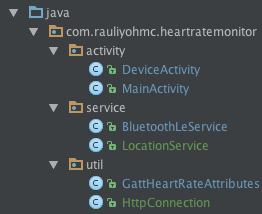
\includegraphics[height=6cm]{graphs/srctree.png} \caption{Organización del código fuente}\label{fig:srctree}
\end{figure}
 
\subsection{Interfaz gráfica} 

    La interfaz gráfica de esta aplicación se ha desarrollado siguiendo las nuevas guías de diseño que incorpora el sistema Lollipop. La versión 5.0 del sistema operativo de Android recomienda una nueva tendencia de diseño, llamada \tit{Material Design} (diseño material), la cual tiene como objetivo crear un lenguaje visual que sintetiza los principios clásicos de buen diseño mediante el uso de la innovación, tal y como su principio rige.

    En concreto se han seguido las recomendaciones para el diseño de los elementos de la lista de dispositivos, la paleta de colores, y la barra de acción o \tit{Action bar} como es comúnmente conocida en el mundo Android.

    En Android hay dos maneras de definir una interfaz gráfica: programáticamente o por archivos de recurso XML. Se ha optado por la segunda opción. Esto disminuye el acoplamiento en el código, aumenta la reusabilidad y la claridad del mismo. Por otra parte, el entorno de desarrollo permite previsualizar el resultado de dichos archivos XML con bastante fidelidad.

 \begin{figure}[h] \centering
    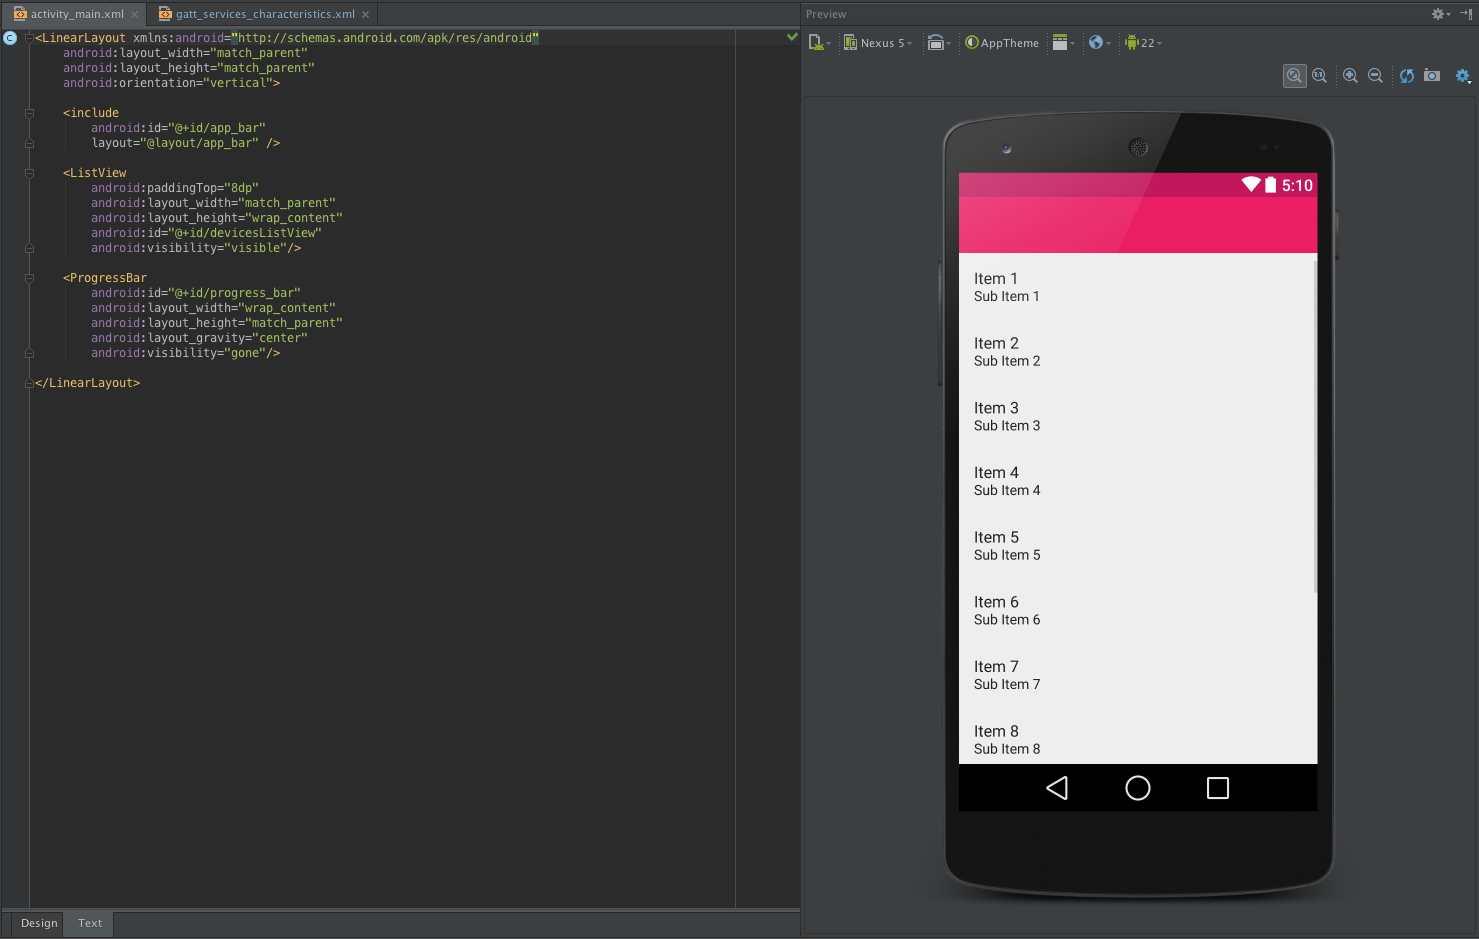
\includegraphics[width=15cm]{graphs/layoutedit.png} \caption{Editor de archivos de recurso XML con vista previa}\label{fig:layoutedit}
\end{figure}

    Para el diseño de los archivos XML se ha hecho uso de la herramienta incorporada para tal propósito en el entorno de desarrollo Android Studio; la cual nos brinda la posibilidad de tener una vista previa del resultado de la descripción en XML que estamos realizando dela interfaz gráfica de usuario. Como ejemplo, en la figura \ref{fig:layoutedit} se puede observar la edición de la interfaz gráfica de usuario de la actividad encargada de mostrar los servicios y características de un sensor en concreto.

	Si así se deseara, también cambe la posibilidad de diseñar las interfaces gráficas de usuario de la aplicación mediante la misma herramienta, pero de una manera completamente visual, tal y como se observa en la figura \ref{fig:layoutvisual}. De esta manera, se sacrifica precisión y control por comodidad y claridad.

	\begin{figure}[h] \centering
	    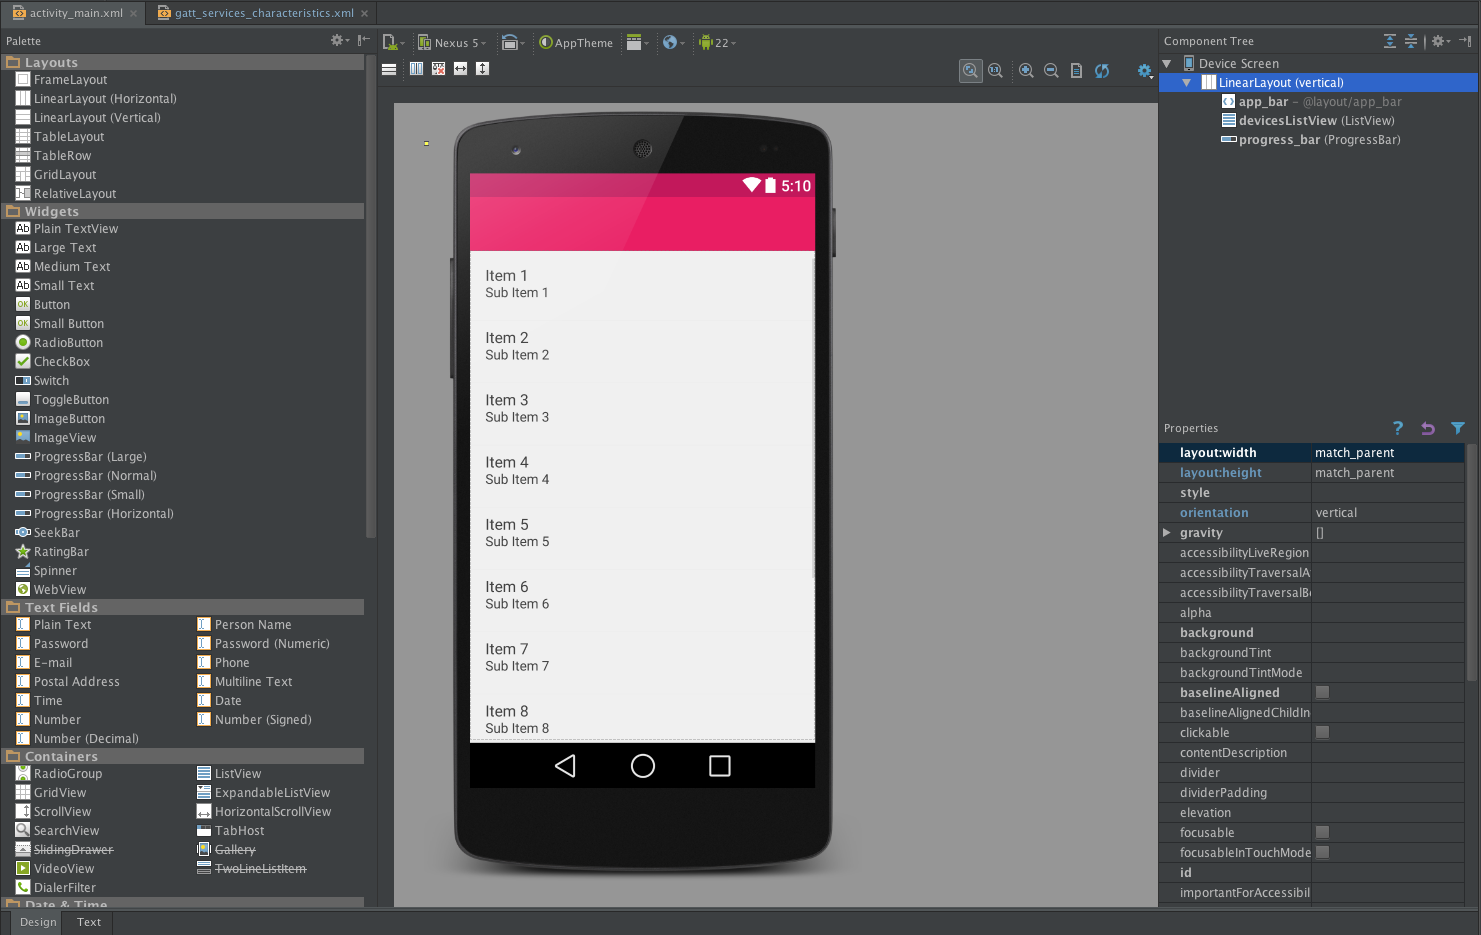
\includegraphics[width=15cm]{graphs/layoutvisual.png} \caption{Edición completamente visual de la interfaz gráfica de usuario de la aplicación}\label{fig:layoutvisual}
	\end{figure}

	Dentro de cada pantalla, la estructuración de los elementos que se observan se realiza a través de layouts. Los layouts pueden definirse como contenedores de una o más vistas, que ayudan al posicionamiento de cada una de ellas dentro de la aplicación así como a controlar el comportamiento de las mismas. Este concepto encaja a la perfección con el anidado de etiquetas de XML. En el ejemplo de la figura \ref{fig:layoutedit}, el código XML es el presente en el extracto \ref{code:layout}. En dicho extracto se puede observar cómo el elemento \ttw{LinearLayout} contiene a 3 elementos. La directiva \ttw{include} nos permite importar fragmentos de xml contenidos en otros archivos, facilitando la modularización y reutilización de código.
	
\begin{listing}[!htpb] 
%\RecustomVerbatimEnvironment{Verbatim}{BVerbatim}{}
\begin{minted}[linenos,numberblanklines,breaklines,frame=lines]{xml}
<LinearLayout
    android:layout_width="match_parent"
    android:layout_height="match_parent"
    android:orientation="vertical">
<include
    android:id="@+id/app_bar"
    layout="@layout/app_bar" />
<ListView
    android:paddingTop="8dp"
    android:layout_width="match_parent"
    android:layout_height="wrap_content"
    android:id="@+id/devicesListView"
    android:visibility="visible"/>
<ProgressBar
    android:id="@+id/progress_bar"
    android:layout_width="wrap_content"
    android:layout_height="match_parent"
    android:layout_gravity="center"
    android:visibility="gone"/>
</LinearLayout>
\end{minted}
\caption{Descripción de la interfaz gráfica de la actividad \ttw{MainActivity}}
\label{code:layout}
\end{listing}
	
	En este caso incluimos la barra de acción, la cual es común en varios de nuestros layouts. \ttw{ListView} hace referencia a una lista con elementos, que representarán los dispositivos BLE encontrados, siendo esta visible cuando la aplicación se inicializa. Por último tenemos un elemento \ttw{ProgressBar}, o barra de progreso, que permanecerá activa cuando la aplicación se encuentre escaneando dispositivos. Como podemos observar cada elemento define sus propios atributos o propiedades, como pueden ser el margen, anchura, altura o alineamiento del widget.

	El atributo \ttw{id} es un identificador único asociado a a cada elemento xml, el cual será usado posteriormente en nuestro código Java para referenciar dichos elementos programáticamente y poder operar con ellos.

\subsubsection{Menús y barra de acción}

La barra de acción, más comúnmente conocida por su versión inglesa \ttw{ActionBar}, es uno de los patrones de diseño más comunes en una aplicación Android. Su función es albergar las funciones importantes y proveer al usuario un fácil, rápido e intuitivo acceso a ellas. La forma de definir los elementos que componen un \ttw{ActionBar} en un determinado instante, así como sus prioridades y jerarquía, es mediante xml, concretamente usando el elemento \ttw{menu} como padre. La figura \ref{fig:actionbar} muestra las acciones de escaneo y detención, las cuales están representadas por los dos iconos de color blanco.

\begin{figure}[h] \centering
	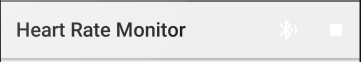
\includegraphics[width=10cm]{graphs/actionbar.png} \caption{Barra de Acción en la actividad principal \ttw{MainActivity}}\label{fig:actionbar}
\end{figure}



%\filbreak

\subsection{Diagrama de flujo} \label{diagramaFlujoAndroid}
	Antes de entrar en detalles técnicos de implementación relacionados con las interacciones que nuestra aplicación Android realiza con el sensor mediante la API de Bluetooth de baja energía, el acceso a servicios de localización y la comunicación con el servidor web, vamos a mostrar un diagrama de flujo completo de la aplicación, para así dotar al lector de una visión general de cómo la aplicación se comporta desde que esta se inicia hasta que esta se finaliza. Este puede ser visualizado en la figura \ref{DiagramaFlujo}.
	
	\filbreak
	
	\begin{figure}[!htbp] \centering
		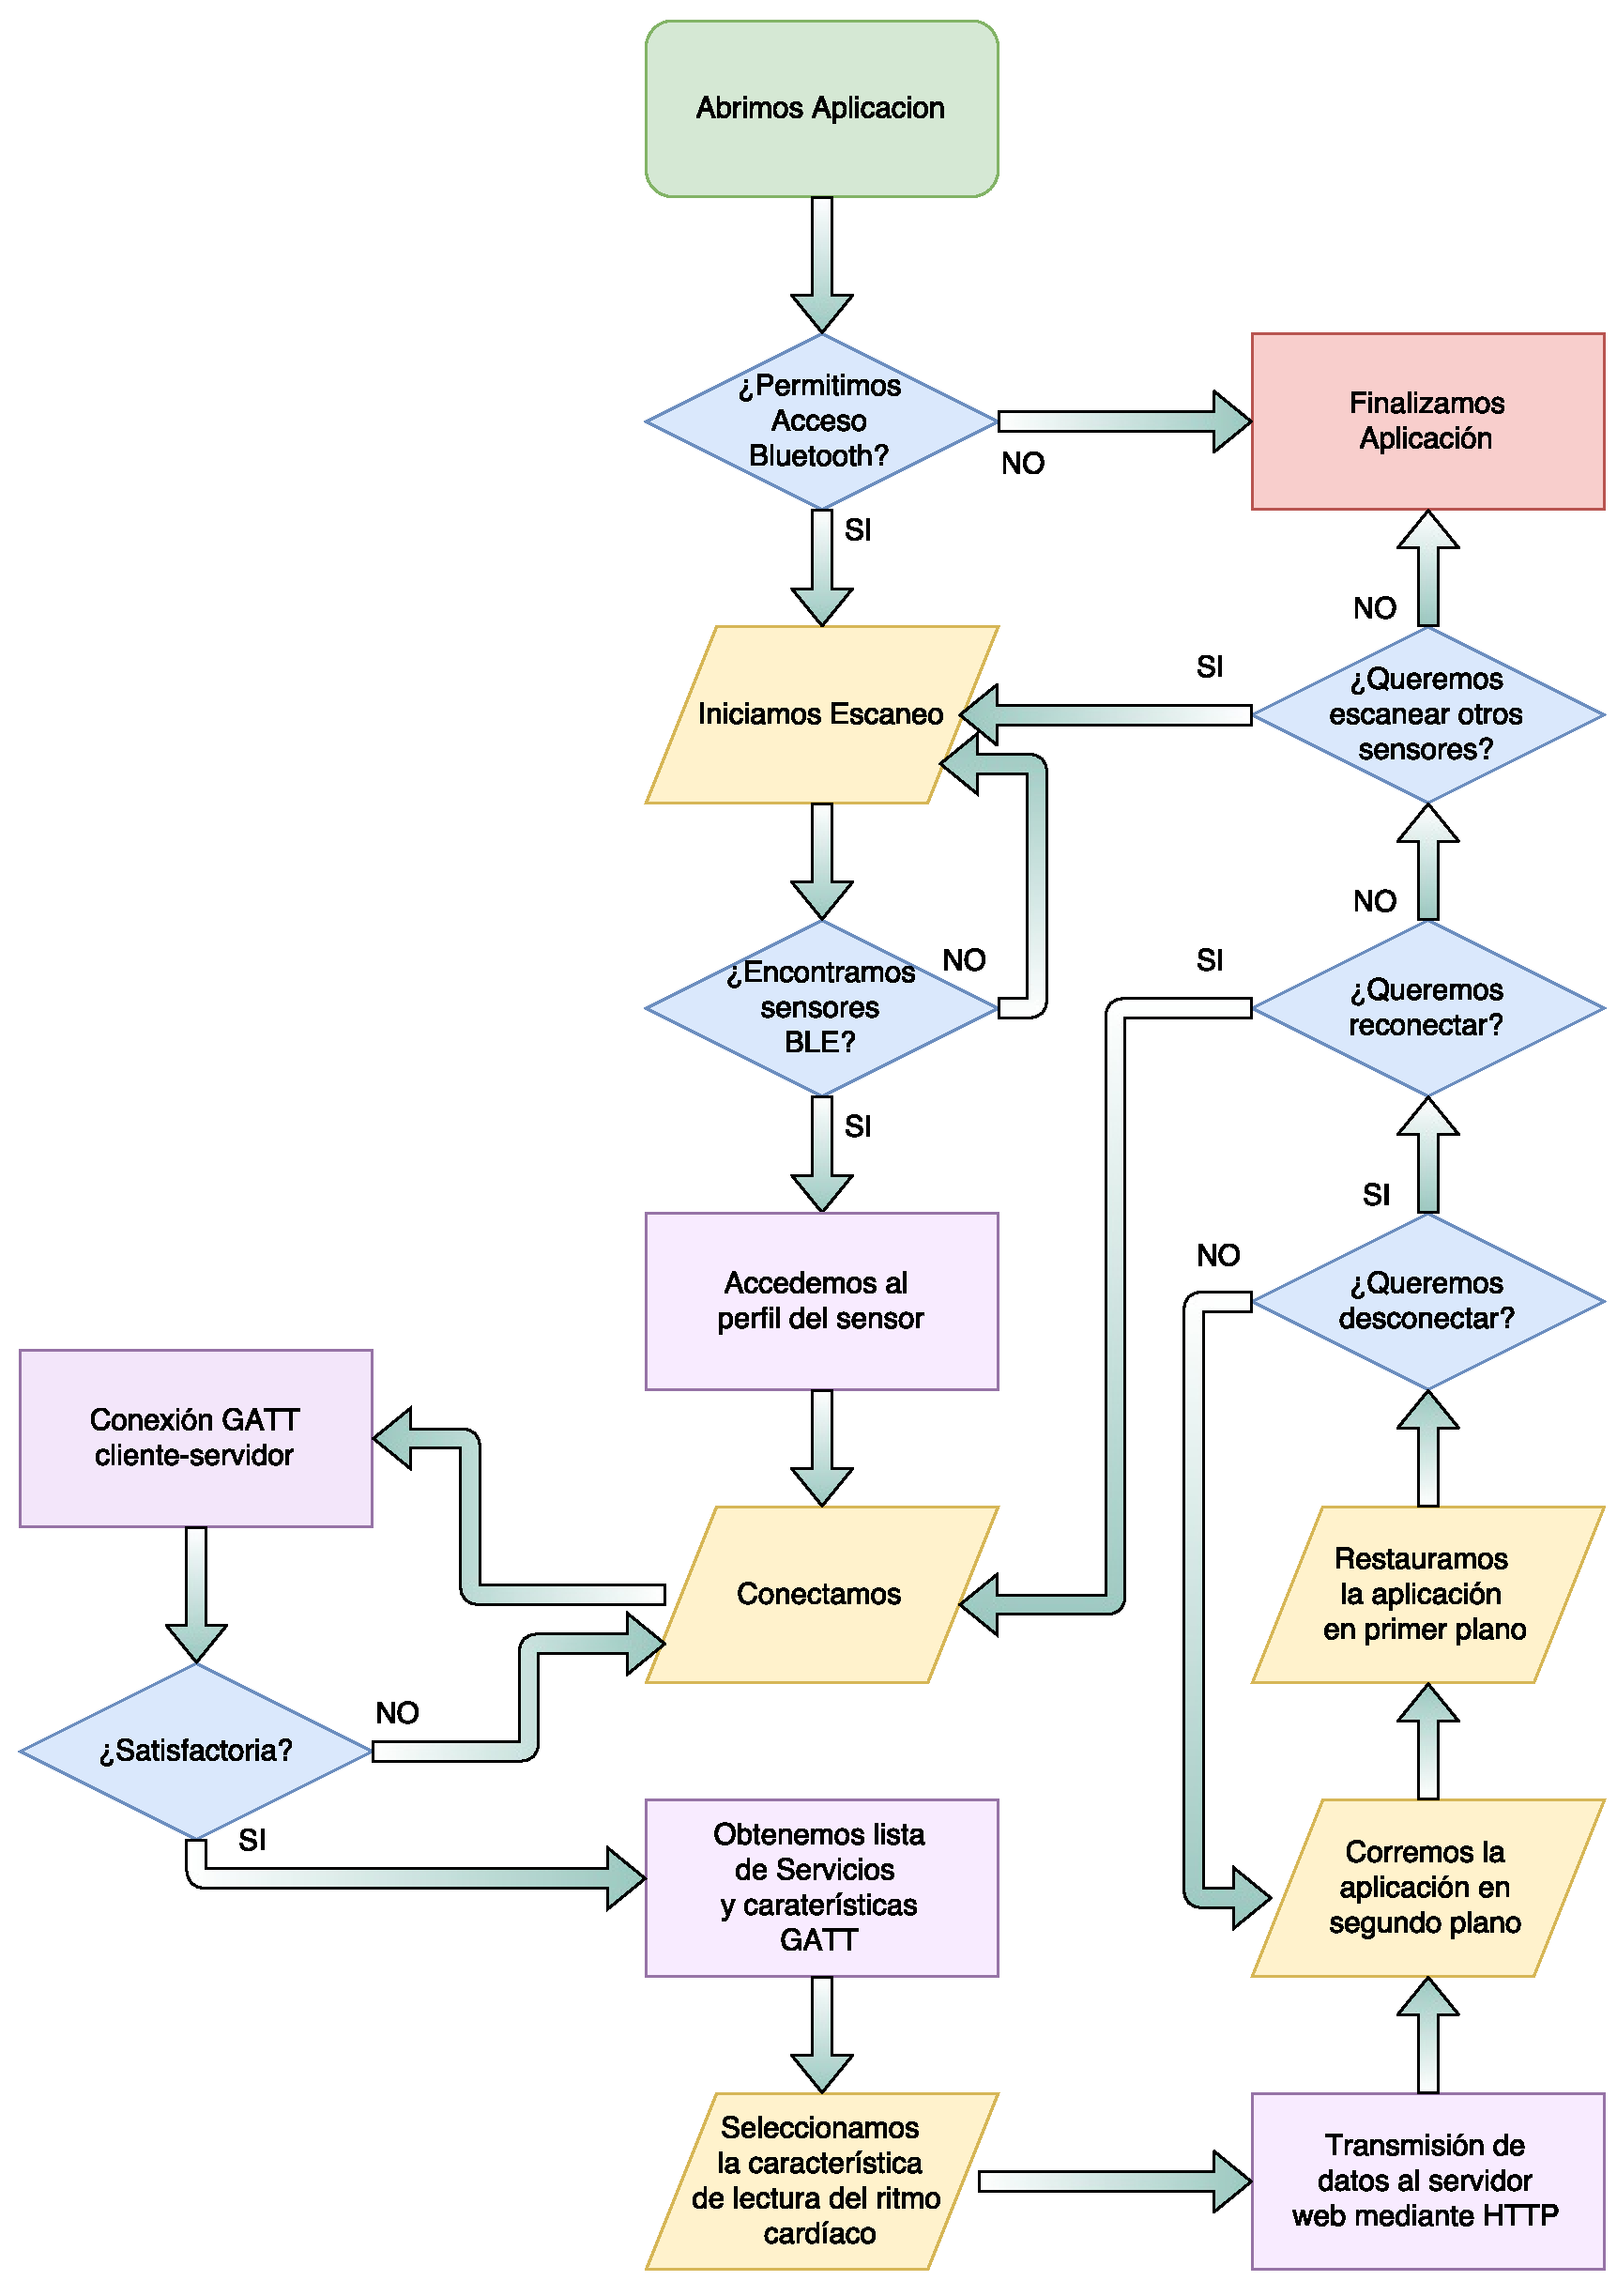
\includegraphics[height=20cm]{graphs/AndroidDiagramaFlujo.pdf} \caption{Diagrama de flujo de la aplicación Android}
		\label{DiagramaFlujo}
	\end{figure}
    
\subsection{Comunicación con el sensor mediante BLE}
	La figura \ref{fig:diagrama:bluetoothhal} muestra los distintos niveles de la arquitectura de Bluetooth en el sistema operativo Android y su interconexión.
	
	
	En el nivel de marco de aplicación, el cual es el nivel en el que nuestras aplicaciones corren, estas usan las clases del paquete \ttw{android.bluetooth.*} para interactuar con el hardware Bluetooth. Internamente, estas clases llaman al proceso Bluetooth a través de un juntador, que es el llamado Binder y lo que permite dicha interconexión.
	
	El servicio del sistema Bluetooth está empaquetado como una Aplicación Android de por sí, e implementa el servicio Bluetooth y los distintos perfiles soportados en Android. Esta aplicación se conecta con la capa \ac{HAL} a través de un \ac{JNI}, el cual es un framework de programación que permite que un programa escrito en Java ejecutado en la máquina virtual java (JVM) pueda interactuar con programas escritos en otros lenguajes como C, C++ y ensamblador.

    El sistema operativo Android provee una \ac{HAL} que conecta todas las \ac{API} de alto nivel con los controladores y hardware subyacentes en cada dispositivo, así como con las posibles extensiones añadidas a la pila de Bluetooth proporcionadas por terceras partes.
    
    \begin{figure}[!htpb] \centering
    	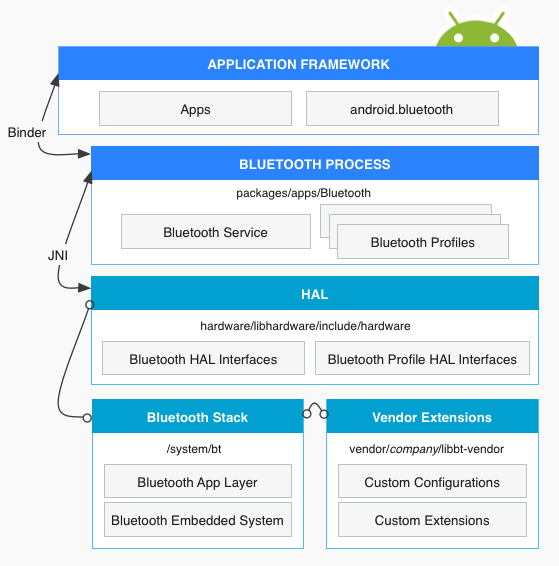
\includegraphics[width=15cm]{graphs/bluetoothandroid.png} \caption{Arquitectura de Bluetooth en Android  \cite{bluetoothhal}}\label{fig:diagrama:bluetoothhal}
    \end{figure}
    
    Lo primero que debemos hacer es declarar en el manifiesto permisos de acceso de la aplicación a Bluetooth, para que así la aplicación pueda utilizar las respectivas APIs y acceder al proceso Bluetooth.
    
    Si el dispositivo Android no soporta BLE, se lo indicaremos al usuario mediante un mensaje informativo, justo al inicializar la aplicación, finalizando esta tan pronto como el mensaje desaparezca.
    
    En el fragmento \ref{code:blePermissions}, vemos el código encargado de dicha función;
    
\begin{listing}[h] 
\begin{minted}[mathescape,linenos,numberblanklines,breaklines,frame=lines]{java}
if (!getPackageManager()
    .hasSystemFeature(PackageManager.FEATURE_BLUETOOTH_LE)) {
        Toast.makeText(this,
            R.string.ble_not_supported,
            Toast.LENGTH_SHORT)
        .show();
finish();
}
\end{minted}
\caption{Detección de soporte BLE en un dispositivo Android}
\label{code:blePermissions}
\end{listing}

Previo a que nuestra aplicación pueda comunicarse a través de BLE, y una vez que hemos comprobado que BLE es soportado en nuestro dispositivo, debemos configurarlo.
Primero necesitamos obtener una instancia de la clase \ttw{BluetoothAdapter}, la cual es requerida para cualquier actividad relacionada con Bluetooth. Esta clase representa el adaptador Bluetooth del dispositivo (la radiofrecuencia Bluetooth). Existe unicamente una instancia compartida a través de toda la aplicación, conocido como \tit{singletone}. Para obtener el adaptador debemos usar \ttw{getSystemService()} para devolver una instancia de \ttw{BluetoothManager}, la cual es finalmente usada para obtener el adaptador.
Como siguiente paso debemos habilitar Bluetooth en nuestro dispositivo. Para ello comprobamos si está actualmente habilitado y si no es así lo habilitamos usando uno de los \ttw{Intent} implícitos que Android provee. Un \ttw{Intent} no es más que una descripción abstracta de una operación que debe ser realizada. Permite de esta forma interactuar con otras actividades, en este caso con la Actividad preinstalada en Android que maneja el controlador Bluetooth. El fragmento \ref{code:bleSettingup} muestra este proceso:

\begin{listing}[h] 
\begin{minted}[mathescape,linenos,numberblanklines,breaklines,frame=lines]{java}
// Inicializa el adaptador Bluetooth
final BluetoothManager bluetoothManager =
    (BluetoothManager) getSystemService(Context.BLUETOOTH_SERVICE);
mBluetoothAdapter = bluetoothManager.getAdapter();
...
// Asegura que Bluetooth esta habilitado en el dispositivo. Si no,
// muestra un dialogo requiriendo al usuario su activacion
if (mBluetoothAdapter == null || !mBluetoothAdapter.isEnabled()) {
    Intent enableBtIntent = 
        new Intent(BluetoothAdapter.ACTION_REQUEST_ENABLE);
    startActivityForResult(enableBtIntent, REQUEST_ENABLE_BT);
}
\end{minted}
\caption{Configuración BLE en Android}
\label{code:bleSettingup}
\end{listing}

Para encontrar dispositivos BLE dentro del alcance de nuestro teléfono Android, debemos usar el método \ttw{startLeScan}. Este método presenta una versión que nos permite especificar los servicios GATT en los cuales estamos interesados como primer parámetro, mediante un arreglo o array de objetos \ttw{UUID}. \ac{UUID} representa un código identificador estándar que se utiliza en el proceso de construcción de software. En el caso del servicio GATT de frecuencia cardíaca, su UUID asociado es el 0000180d-0000-1000-8000-00805f9b34fb. El segundo parámetro de la función es un objeto \ttw{BluetoothAdapter.LeScanCallback}. Debemos implementar esta retrollamada, porque es la forma en la que los resultados de escaneo serán devueltos. Debido a que escanear dispositivos consume bastante batería, debemos ser cuidadosos y seguir los siguientes criterios:

\begin{itemize}
\item Tan pronto como encontremos el dispositivo deseado, paramos de escanear.
\item No debemos escanear en bucle, fijando un límite de tiempo para el escaneo.
\end{itemize}

La función encargada de empezar y parar el escaneo es la mostrada en el fragmento \ref{code:bleScan}.

\begin{listing}[h] 
\begin{minted}[mathescape,linenos,numberblanklines,breaklines,frame=lines]{java}
private static final long SCAN_PERIOD = 10000; 
private static final UUID[] heartRateGattServices = new UUID[1];
heartRateGattServices[0] = 
    UUID.fromString("0000180d-0000-1000-8000-00805f9b34fb");
...
private void scanLeDevice(final boolean enable) {
    if (enable) {
        // Detiene el escaneo despues del tiempo predefinido, 10s aqui
        handler.postDelayed(new Runnable() {
             @Override
             public void run() {
                 scanning = false;
                 bluetoothAdapter.stopLeScan(leScanCallback);
             }
        }, SCAN_PERIOD);
        scanning = true;
        bluetoothAdapter
            .startLeScan(heartRateGattServices, leScanCallback);
    } else {
        scanning = false;
        bluetoothAdapter
            .stopLeScan(heartRateGattServices, leScanCallback);
    }
 ...
}
\end{minted}
\caption{Proceso de escaneo de dispositivos BLE en Android}
\label{code:bleScan}
\end{listing}

El fragmento \ref{code:bleScanCallback} muestra un ejemplo de implementación de la interfaz \\ \ttw{BluetoothAdapter.LeScanCallback}, usada para entregar resultados de escaneo BLE.

\begin{listing}[h] 
\begin{minted}[mathescape,linenos,numberblanklines,breaklines,frame=lines]{java}
private LeDeviceListAdapter deviceListAdapter;
...
//Retrollamada de escaneo BLE
private BluetoothAdapter.LeScanCallback leScanCallback =
           new BluetoothAdapter.LeScanCallback() {
    @Override
    public void onLeScan(final BluetoothDevice device, int rssi,
            byte[] scanRecord) {
        runOnUiThread(new Runnable() {
            @Override
            public void run() {
                deviceListAdapter.addDevice(device);
                deviceListAdapter.notifyDataSetChanged();
            }
        });
    }
};		
\end{minted}
\caption{Implementación de la interfaz BluetoothAdapter.LeScanCallback}
\label{code:bleScanCallback}
\end{listing}
Para garantizar que las operaciones GATT servidor-cliente no se ven interferidas por otras funciones de la aplicación, se ha optado por crear un servicio que corra en segundo plano. Este responde a los comandos de la aplicación en primer plano, tal y como se explicó en el apartado \ref{ssec:teo:svc}.
Este servicio, \ttw{BluetoothLeService}, será del tipo \ttw{Bound} y estará adherido a la actividad \ttw{DeviceActivity}, la cual se encarga de mostrar los datos relativos al sensor que nos queremos conectar, tal y como podíamos ver en los bosquejos \ref{fig:mockup:desconectado} y \ref{fig:mockup:conectado} en sus estados desconectado y conectado respectivamente.
Recordemos que un servicio del tipo \ttw{Bound} está activo durante el tiempo en que la actividad \ttw{DeviceActivity} esté adherida a él y que es destruido cuando dicha actividad se desadhiere.

Una vez pulsemos en ``Conectar'' en dicha actividad, se llamará en código al método \ttw{connectGatt()} dentro del servicio. Este método recibe 3 parámetros, un objeto \ttw{Context}, en este caso el contexto del servicio, un booleano indicando si debemos conectarnos automáticamente al dispositivo BLE tan pronto como este se encuentre disponible, y una retrollamada del tipo \ttw{BluetoothGattCallback}. \\
\ttw{bluetoothGatt = device.connectGatt(this, false, bluetoothGattCallback);}

Esta expresión devuelve una instancia de la clase \ttw{BluetoothGatt}, la cual podemos usar para llevar a cabo operaciones GATT del lado del cliente, o sea la aplicación Android. El tercer parámetro \ttw{bluetoothGattCallback}, instancia de la clase abstracta \ttw{BluetoothGattCallback}, es una retrollamada utilizada para entregar resultados al cliente, tales como el estado de la conexión o cualquier futura operación GATT del lado del cliente. La forma de definirla es mediante la implementación de su clase Abstracta, en particular aquellos métodos en los cuales estamos interesados. Estos métodos serán los listados a continuación:
\begin{itemize}
	\item \ttw{onConnectionStateChange} \\
	Retrollamada que será ejecutada cuando el estado de la conexión GATT cambie. En nuestro caso, en cuanto la conexión con el sensor se haya establecido, procederemos a descubrir los servicios GATT ofrecidos por este. Una vez que nos hayamos desconectado enviaremos una petición HTTP al servidor web para informar al usuario apropiadamente.
	
	\item \ttw{onServicesDiscovered} \\
	Retrollamada que será ejecutada justo cuando el proceso de descubrir los servicios GATT ofrecidos por el sensor haya finalizado. Aquí procederemos a actualizar la interfaz de usuario en la actividad \ttw{DeviceActivity}, mostrando una lista expandible con los servicios GATT ofrecidos.
	
	\item \ttw{onCharacteristicRead} \\
	Una vez que seleccionemos la característica lectura del ritmo cardíaco, dentro del servicio del ritmo cardíaco, procederemos a recibir periódicamente y con una frecuencia en torno al segundo datos provenientes del sensor BLE. Cada vez que recibamos un nuevo valor de frecuencia cardíaca, esta retrollamada será ejecutada, y llevaremos a cabo el envío de dicho valor al servidor web.
\end{itemize}

El proceso de análisis sintáctico y gramatical de los datos que nos llegan del sensor (parsing) se lleva a cabo siguiendo las especificaciones del perfil Bluetooth de la medida de ritmo cardíaco\footnote{Para consultar las especificaciones completas, se invita al lector a visitar \mbox{\url{https://developer.bluetooth.org/gatt/characteristics/Pages/CharacteristicsHome.aspx }}}. Estos datos serán recibidos por la aplicación Android como una agrupación de bytes. Nuestro objetivo es obtener un número entero legible es por lo que debemos transformar  los datos. El código encargado de la transformación es el mostrado en el fragmento \ref{code:bleParsing}.

\begin{listing}[h] 
\begin{minted}[mathescape,linenos,numberblanklines,breaklines,frame=lines]{java}
if (UUID_HEART_RATE_MEASUREMENT.equals(characteristic.getUuid())) {
    int flag = characteristic.getProperties();
    int format = -1;
    if ((flag & 0x01) != 0) {
        format = BluetoothGattCharacteristic.FORMAT_UINT16;
    } else {
        format = BluetoothGattCharacteristic.FORMAT_UINT8;
    }
    final int heartRate = characteristic.getIntValue(format, 1);
} 
\end{minted}
\caption{Parsing para el perfil de ritmo cardíaco}
\label{code:bleParsing}
\end{listing}

En la actividad \ttw{DeviceActivity} usaremos un objeto de la clase \ttw{BroadcastReceiver} para poder recibir eventos desde el Servicio y así actualizar la interfaz de usuario acordemente.

Por último, una vez que la aplicación ha terminado la interacción con el sensor BLE, debemos liberar conexiones y recursos apropiadamente. En nuestro caso, el proceso de cerrar la conexión ocurrirá cuando pulsemos el botón ``Desconectar'' en la barra de acción. De esta forma la actividad \ttw{Device Activity} se desconectará del servicio y la conexión GATT cliente-servidor será cerrada.

\subsection{Ubicación}

Para obtener la ubicación absoluta del dispositivo móvil, la aplicación se comunica con los \ac{GMS}. Estos no solo actúan como una capa de abstracción del hardware \ac{GPS} del dispositivo, sino que además proveen servicios de valor añadido. Algunos de los beneficios incluyen un menor tiempo de precalentamiento, localización por redes Wi-Fi y optimización del consumo energético.
No obstante, antes de hacer uso de los GMS, es necesario configurar el proyecto para que obtenga como dependencias las librerías pertinentes. Gracias al sistema de compilación de Gradle, este paso es sumamente sencillo.


\begin{listing}[h] 
%\RecustomVerbatimEnvironment{Verbatim}{BVerbatim}{}
\begin{minted}[mathescape,linenos,numberblanklines,breaklines,frame=lines]{groovy}
dependencies {
    compile fileTree(dir: 'libs', include: ['*.jar'])
    compile 'com.android.support:appcompat-v7:21.0.3'
    compile 'com.android.support:recyclerview-v7:+'
    compile 'com.google.android.gms:play-services:7.3.0'
}
\end{minted}
\caption{Sección de dependencias dentro del archivo \ttw{build.gradle}}
\label{code:buildeps}
\end{listing}

Los \ac{GMS} en su versión más reciente se han fragmentado, así que solo es necesario declarar como dependencias las partes que sean necesarias en el proyecto, para evitar sobrecargar la aplicación. Las dependencias se añaden editando el archivo \ttw{build.gradle}. Para utilizar la parte de ubicación de los GMS, se añade la línea 4 del fragmento \ref{code:buildeps}, dado que ubicación se encuentra en la parte general de las librerías. Las dependencias son añadidas con el descriptor Maven\footnote{El funcionamiento de la herramienta Maven y el sistema de gestión de proyectos de software asociado quedan fuera del ámbito de este proyecto. No obstante, se invita al lector a visitar \mbox{\url{maven.apache.org} para conocer más acerca de los mismos.}} del paquete, siguiendo el esquema \ttw{paquete-padre:librería:versión}, y son descargadas del repositorio central de Maven.

\begin{figure}[h] \centering
\begin{tikzpicture}[node distance = 4cm, auto]
    % Place nodes
    \node [block] (app) {Device \\ Activity};
    \node [block, right of=audio] (loc) {Servicio de\\ localización};
    \node [block, right of=loc] (gms) {GMS};
    \node [block, below of=app] (ble) {Servicio BLE};
    \node [block, below of=loc] (web) {Cliente HTTP};
    
     %Draw edges
    \path [line] (app) -- (loc);
    \path [line] (loc) -- (gms);
    \path [line] (gms) -- (loc);
    \path [line] (app) -- (ble);
	\path [line] (ble) -- (app);    
	\path [line] (loc) -- (web);
	\path [line] (ble) -- (web);
	\path [line] (web) -- (ble);
	\path [line] (web) -- (loc);
\end{tikzpicture}
\caption{Diagrama de interacción de la aplicación y los servicios}\label{fig:diagrama:servicios}
\end{figure}

Para comunicarse con los \ac{GMS}, es utilizado un servicio en segundo plano por los mismos motivos que en el apartado anterior de comunicación con el sensor BLE. De hecho, es un servicio intermedio, ya que la obtención en sí de la posición la realiza el servicio \ac{GMS}. La interacción de la aplicación con los distintos servicios se puede observar en el diagrama \ref{fig:diagrama:servicios}. El servicio de localización creado en la aplicación se conecta a los \ac{GMS}, solicita actualizaciones y las pone a disponibilidad del resto de la aplicación de la manera mostrada en \ref{code:location}.

\begin{listing}[h] 
%\RecustomVerbatimEnvironment{Verbatim}{BVerbatim}{}
\begin{minted}[mathescape,linenos,numberblanklines,breaklines,frame=lines]{java}
googleApiClient = new GoogleApiClient.Builder(this)
    .addConnectionCallbacks(this)
    .addOnConnectionFailedListener(this)
    .addApi(LocationServices.API)
    .build();
createLocationRequest();
googleApiClient.connect();
\end{minted}
\caption{Solicitud de conexión a los GMS.}
\label{code:location}
\end{listing}

\subsection{Comunicación con el servidor web}
Para enviar al servidor web el valor de frecuencia cardíaca y la ubicación del usuario, decidimos hacer uso de las clases 
\ttw{httpClient} y \ttw{httpPost} en Android, las cuales implementan el protocolo HTTP y el método HTTP POST respectivamente, proporcionándonos una API flexible y fácil de usar.
Con tal propósito se creo una clase en java encargada de todas las operaciones HTTP, \ttw{HttpConnection}, la cual contiene dos métodos, uno para enviar el valor de frecuencia cardíaca y otro para enviar la localización en forma de valores de longitud y latitud. El fragmento \ref{code:httpHeartRate} muestra el primero de los métodos:

\begin{listing}[h] 
%\RecustomVerbatimEnvironment{Verbatim}{BVerbatim}{}
\begin{minted}[mathescape,linenos,numberblanklines,breaklines,frame=lines]{java}
public void sendHeartRateToWebServer(int heartRate){
	...
    JSONObject jsonObject = new JSONObject();
    // Le decimos al servidor de desconectar enviando el valor -1
    if(heartRate == -1){
        jsonObject.put("emitting", "false");
    } else {
        jsonObject.put("emitting", "true");
    }
    jsonObject.put("heartRate", heartRate);
    StringEntity se = new StringEntity(jsonObject.toString());
    httpPost.setEntity(se);
    httpPost.setHeader("Accept", "application/json");
    httpPost.setHeader("Content-type", "application/json");
    HttpResponse httpResponse = httpClient.execute(httpPost);
    ...
} 
\end{minted}
\caption{Método para el envío de valores de frecuencia cardíaca al servidor web}
\label{code:httpHeartRate}
\end{listing}

En primer lugar creamos un objeto \ac{JSON}, que no es mas que una tabla hash o diccionario con claves y valores. Adoptamos el convenio de enviar el valor ``-1'' como frecuencia cardíaca al servidor, para comunicarle que nos hemos desconectado del pulsómetro. Utilizamos la clase \ttw{HttpPost} para efectuar peticiones de tipo POST al servidor. De esta forma podemos enviar datos al servidor en el cuerpo del mensaje de la solicitud HTTP. La ejecución de la petición se produce justo al llamar al método \ttw{connect} de la clase \ttw{HttpClient}.

El fragmento \ref{code:httpLocation} muestra el segundo de estos métodos.

Cabe destacar que el envío de valores de frecuencia cardíaca se realiza aproximadamente cada segundo mientras que comprobamos si existe una actualización en la ubicación del usuario cada 2 minutos, ya que la localización no es tan propensa a cambiar tan rápidamente y así realizamos un ahorro considerable de consumo.

\begin{listing}[h] 
%\RecustomVerbatimEnvironment{Verbatim}{BVerbatim}{}
\begin{minted}[mathescape,linenos,numberblanklines,breaklines,frame=lines]{java}
public void sendLocationToWebServer(String latitude, String longitude) {
	...
    JSONObject jsonObject = new JSONObject();
    jsonObject.put("latitude", latitude);
    jsonObject.put("longitude", longitude);
    StringEntity se = new StringEntity(jsonObject.toString());
    httpPost.setEntity(se);
    httpPost.setHeader("Accept", "application/json");
    httpPost.setHeader("Content-type", "application/json");
    HttpResponse httpResponse = httpClient.execute(httpPost);
    ...
}
	
\end{minted}
\caption{Método para el envío de valores de localización al servidor web}
\label{code:httpLocation}
\end{listing}


\section{Aplicación web} 

\subsection{Entorno de desarrollo integrado}
En el mundo de desarrollo web moderno, es muy común recurrir a simples editores de texto para crear y estructurar los distintos archivos que compondrán nuestra aplicación web, usar extensiones (plugins) para realizar tareas como análisis sintáctico del código en un lenguaje específico o proporcionar  plantillas o \tit{snippets} de código y hacer uso del terminal para el proceso de interpretación y compilación del código.
Entre los múltiples editores de texto que se pueden adquirir mediante descarga gratuita, hemos decidido usar Atom, un proyecto de código abierto creado por el equipo de GitHub.
Atom es en editor multiplataforma, es decir, lo tenemos disponible en Windows, MAC OS X y en GNU/Linux y es muy fácil de instalar. A nivel informativo Atom ha sido escrito en C++, Node.js, CoffeeScript, JS, CSS y HTML. De hecho está basado en Chromium, que es un proyecto de navegador web de código abierto, a partir del cual se basa el código fuente de Google Chrome y utiliza la licencia libre MIT License. Permite la instalación de módulos, extensiones y temas para así aumentar sus posibilidades y es fácilmente configurable.

La figura \ref{fig:atom} muestra la versión más actual de Atom en el momento de la escritura de dicha memoria.

\begin{figure}[h] \centering
	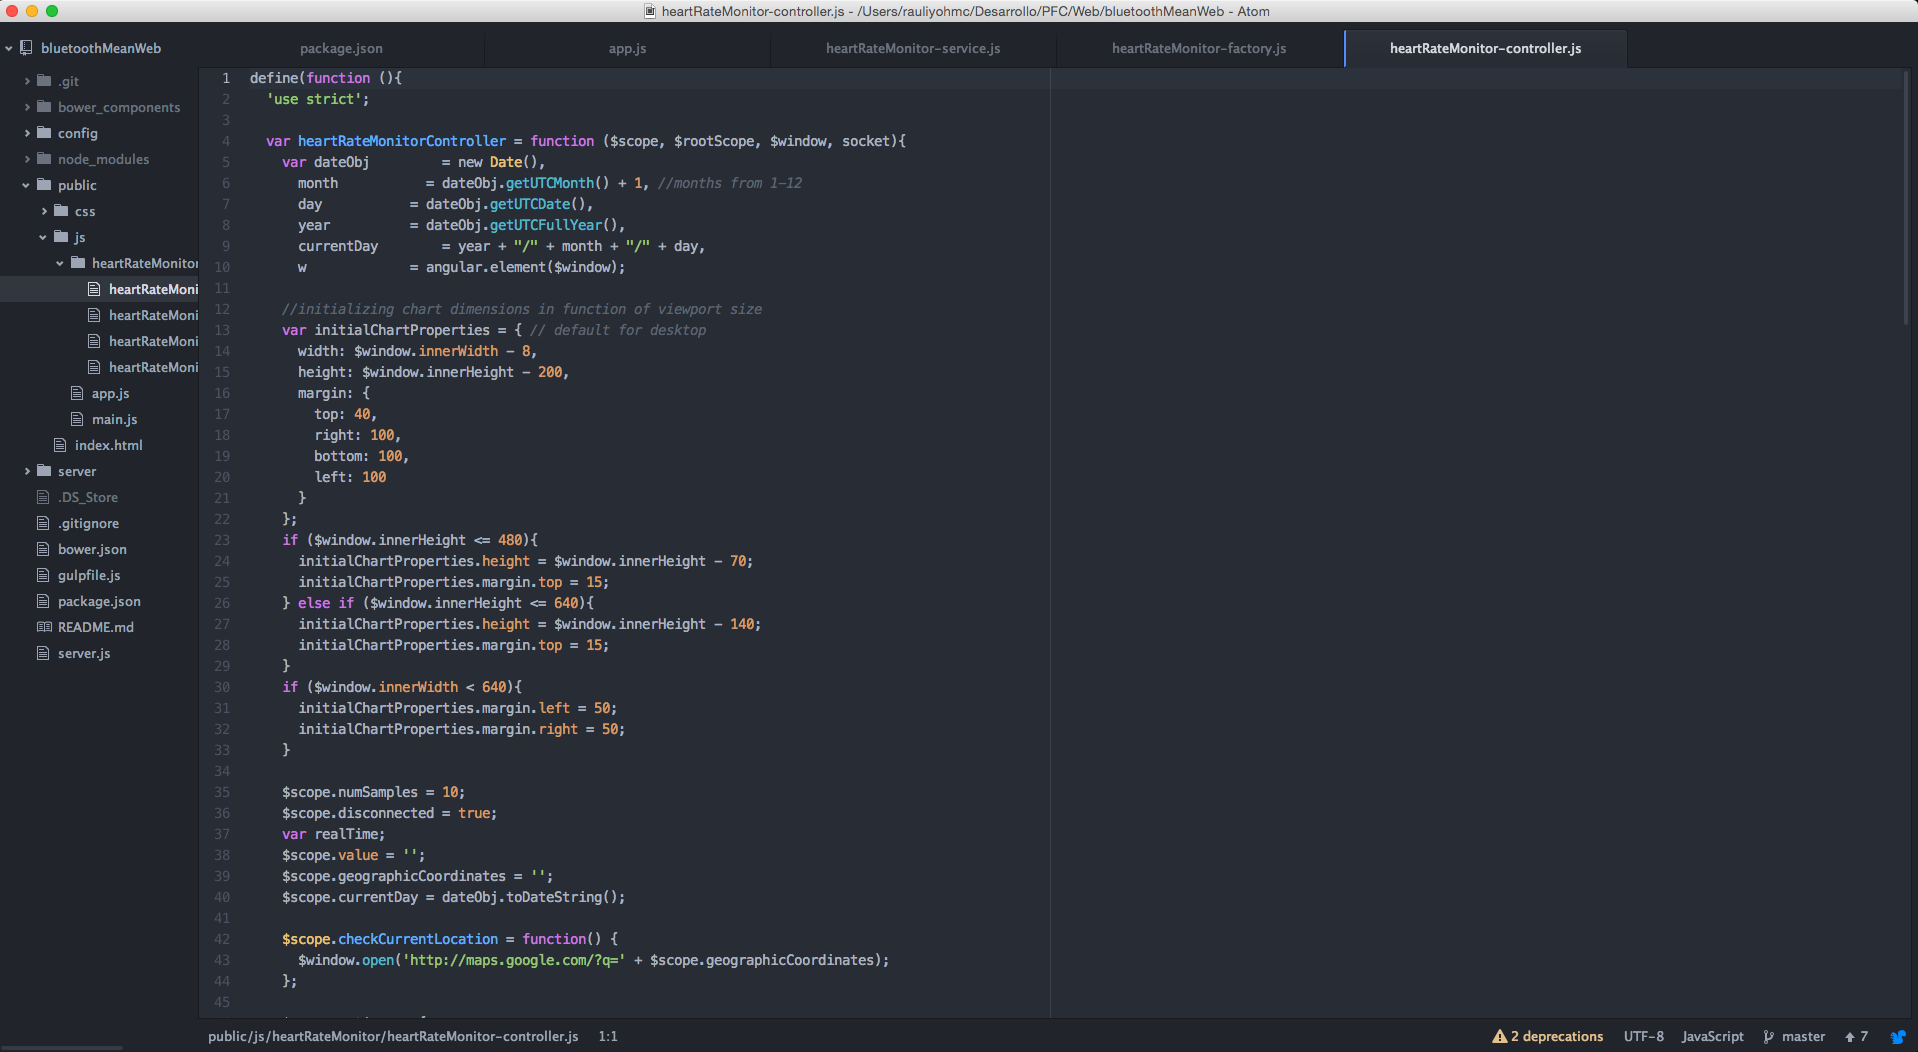
\includegraphics[width=15cm]{graphs/atom.png} \caption{Entorno de desarrollo Atom}\label{fig:atom}
\end{figure}

\subsection{Estructura del código}
La figura \ref{fig:webEstructuraGlobal} muestra la estructura a nivel genérico de nuestra aplicación web. A continuación pasamos a explicar cada una de las partes relevantes:

\begin{figure}[h] \centering
	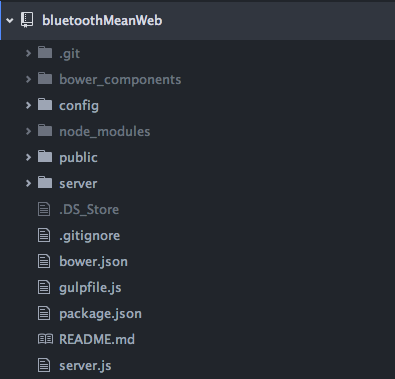
\includegraphics[height=10cm]{graphs/webEstructuraGlobal.png} \caption{Estructura global de la aplicación web}\label{fig:webEstructuraGlobal}
\end{figure}

\begin{description}
\item[bower\_components] \\ Esta carpeta albergará todos los módulos y librerías externas usadas para el desarrollo de la parte cliente, interfaz visual, o \tit{frontend} de la aplicación, tales como la librería \ttw{AngularJS} para el JavaScript del lado del cliente, \ttw{d3} para la creación de las gráficas o \ttw{RequireJS} para la modularización del código.
\item[node\_modules] \\ Es el equivalente a bower\_components, pero para la parte dedicada al servidor. Incluye módulos como \ttw{Express} para la creación del servidor web y las distintas rutas, \ttw{Mongoose} para el manejo de bases de datos o \ttw{Socket.io} para el uso de web sockets.
\item[package.json y bower.json] \\ Estos archivos especifican los distintos módulos requeridos por la aplicación para que esta funcione correctamente, es decir, las dependencias en términos de módulos, así como sus correspondientes versiones. Pueden incluir también instrucciones de código (scripts), para ser ejecutados antes o después de ciertos procesos. Cualquier usuario que quiera correr la aplicación localmente deberá en primer lugar descargarse el código fuente y en segundo lugar instalar todas las dependencias mediante el uso de los comandos \ttw{npm install} o \ttw{bower install}.
Nótese la flexibilidad y rapidez para correr una aplicación usando NodeJS como plataforma de desarrollo web.
\item[config] \\ Contiene archivos con credenciales para el acceso a la base de datos y al cliente de correo electrónico para el envío de notificaciones. Su visibilidad es privada.
\item[server.js] \\ Es el punto de entrada de la aplicación web. Mediante el comando  \ttw{node server}, se correrá la aplicación en la plataforma Node.
\item[server] \\ Contiene toda la lógica del servidor, como la interacción de este con la base de datos, emisión de mensajes a través de una conexión socket y notificaciones a través de un cliente de e-mail entre otros. También proporciona una RESTful API, para que la aplicación Android pueda interactuar y enviar información al servidor.
\item[public] \\ Se refiere a todos los archivos que serán entregados al cliente web, es decir cualquier navegador, una vez que accedamos a la página principal. En este caso todos los archivos html, css y Javascript del lado del cliente.
\end{description}

\subsection{Diagrama de flujo}
Tal y como hicimos con la aplicación Android en el apartado \ref{diagramaFlujoAndroid}, en esta sección mostraremos el diagrama de flujo funcional del servidor web. Este se ilustra en la figura \ref{DiagramaFlujoWeb}, el cual proporciona una visión general de cómo reacciona el servidor ante las distintas solicitudes POST recibidas y qué acciones lleva a cabo dependiendo del tipo de esta, incluyendo respuestas HTTP con código informativo al cliente, interacciones con la base de datos y lógica a ejecutar relacionada con el sistema de notificaciones.

\begin{figure}[!htbp] \centering
	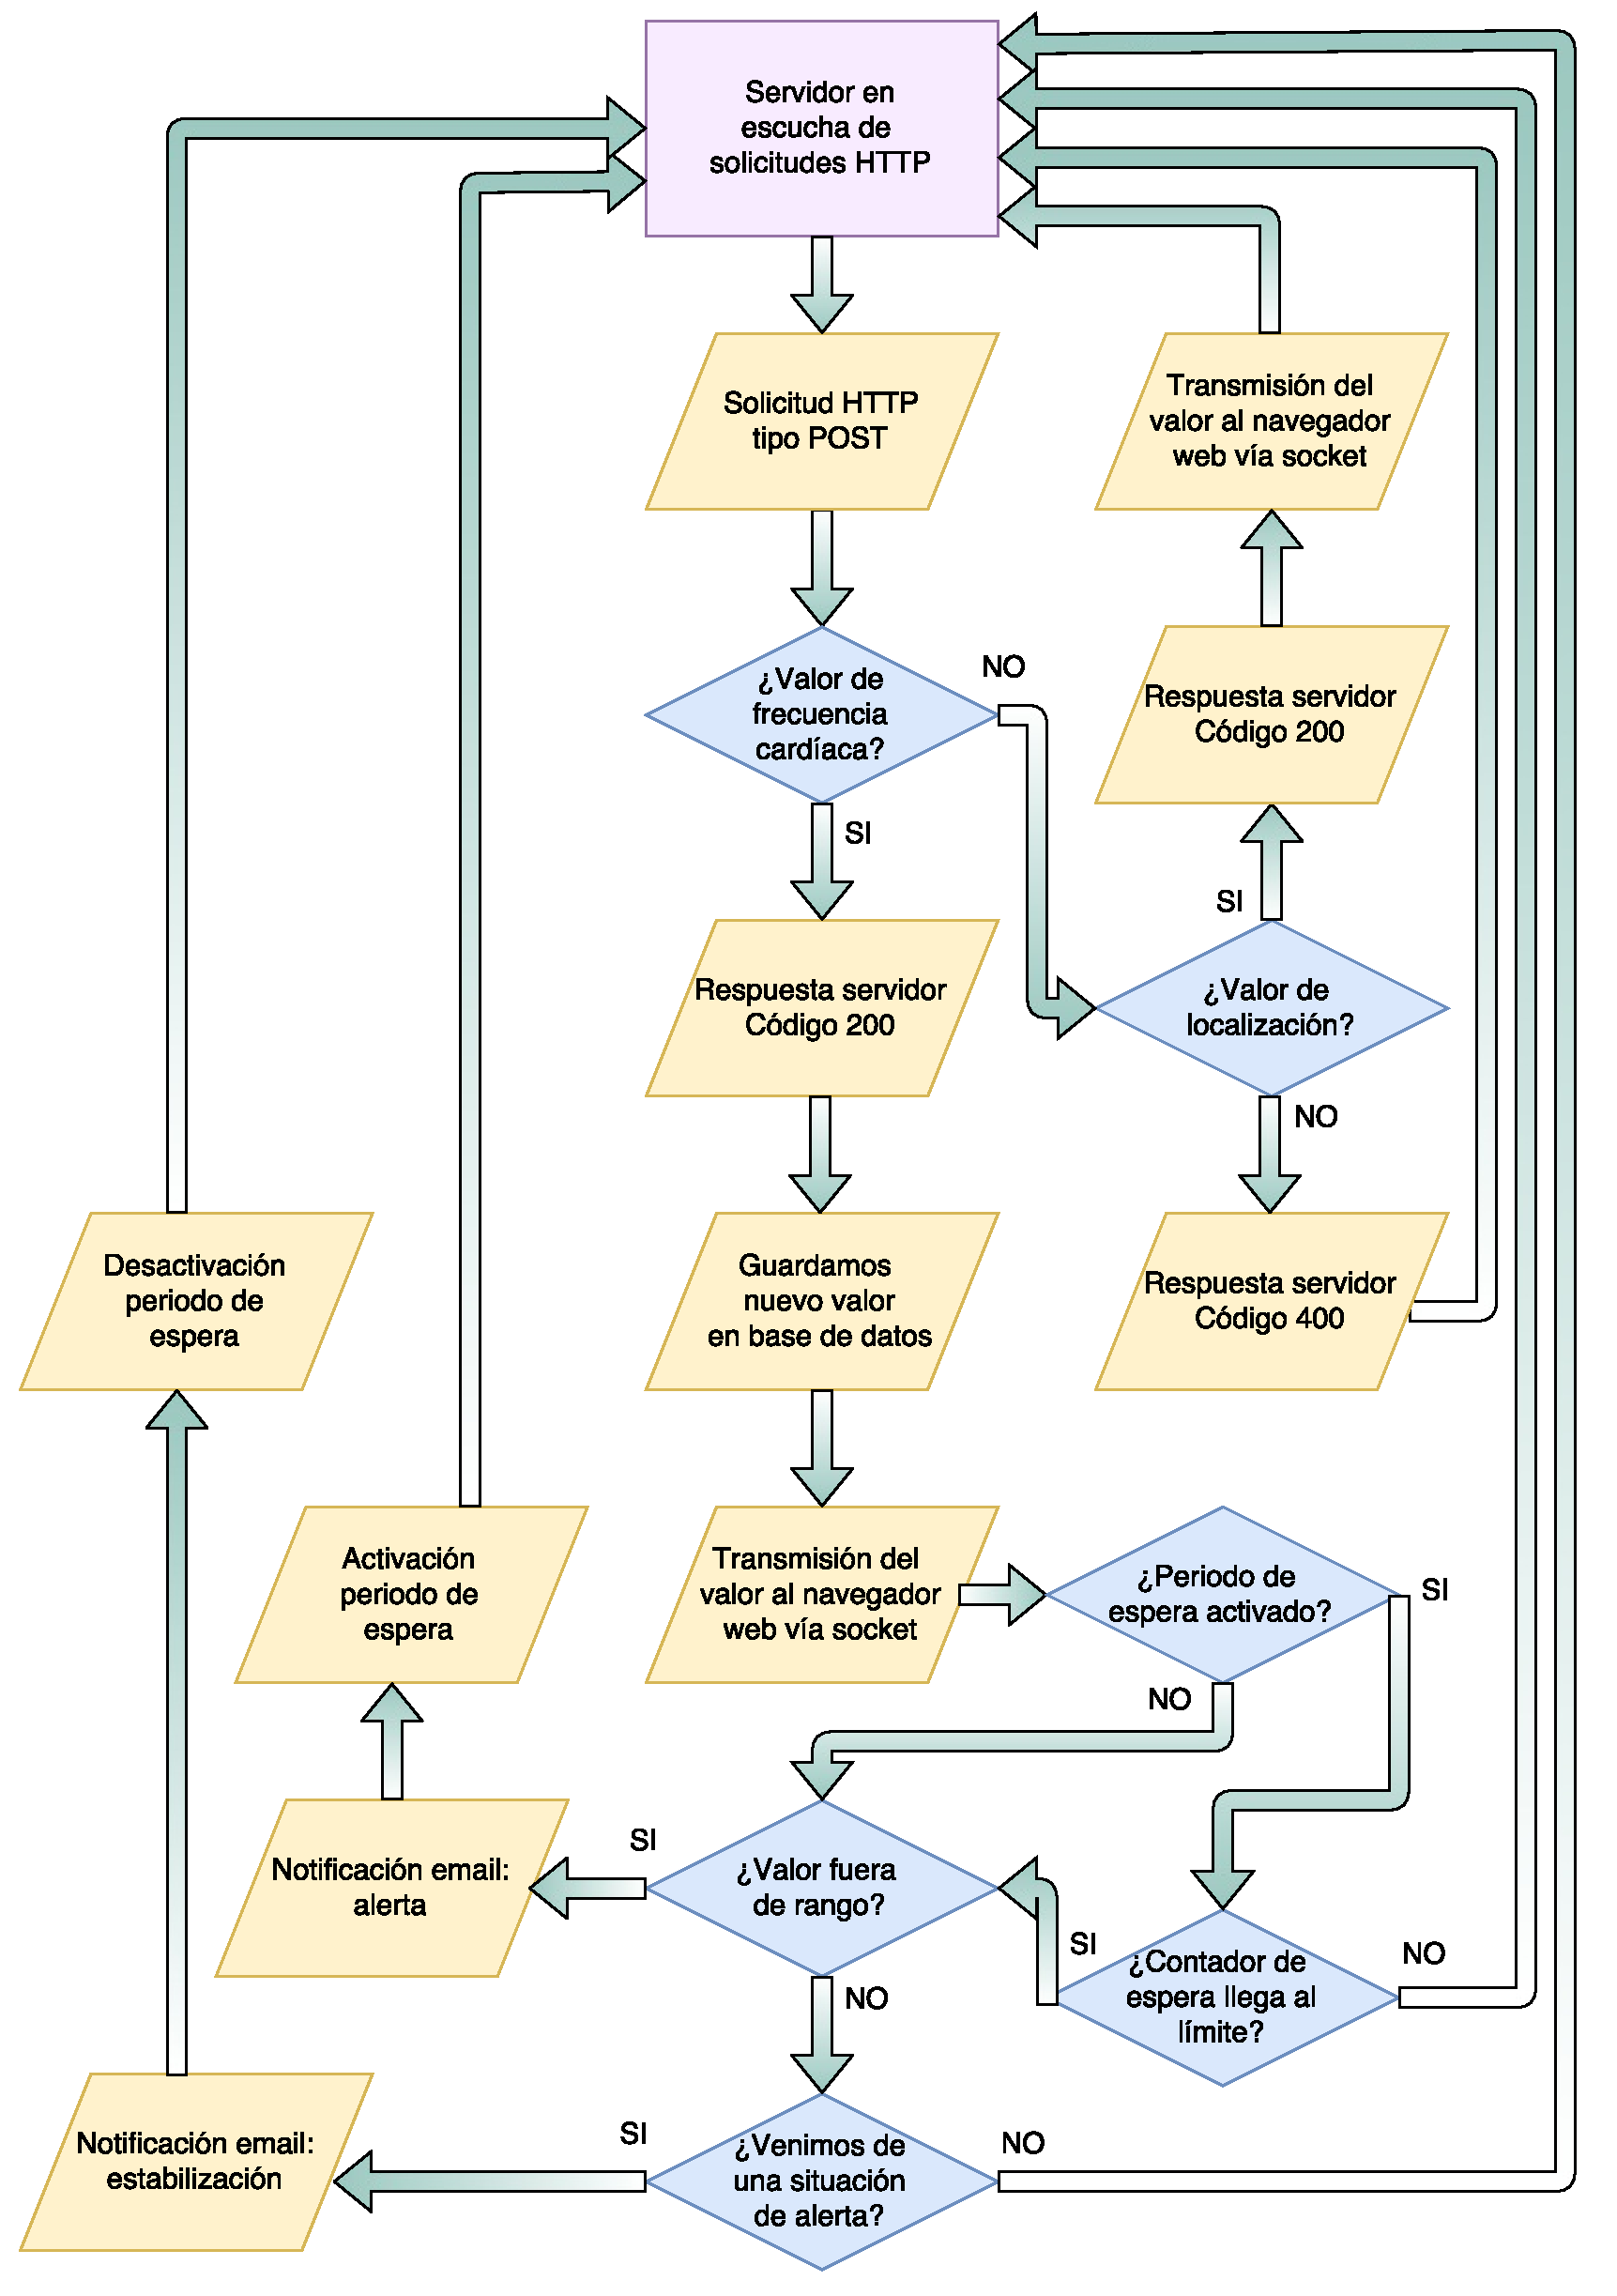
\includegraphics[height=20cm]{graphs/webDiagramaFlujo.pdf} \caption{Diagrama de flujo del servidor web}
	\label{DiagramaFlujoWeb}
\end{figure}



\subsection{Servidor}
\label{cap:Servidor}
Tal y como mencionamos en la sección anterior, el punto de entrada a la aplicación es el archivo \ttw{server.js}. Vamos a desglosar el código involucrado en la configuración básica del servidor y las rutas usando el módulo Express. Éste es el mostrado en el fragmento \ref{code:webExpress}.

\begin{listing}[h] 
%\RecustomVerbatimEnvironment{Verbatim}{BVerbatim}{}
\begin{minted}[mathescape,linenos,numberblanklines,breaklines,frame=lines]{javascript}
var app = express();
// Sirve contenido estatico contenido en la carpeta public
app.use(express.static(__dirname + '/public'));
app.use('/bower_components', 
          express.static(__dirname + '/bower_components'));
app.use('/node_modules',  express.static(__dirname + '/node_modules'));
// Modulo usado para manejar solicitudes de tipo POST
app.use(bodyParser());
// Configuracion del socket
var server = http.createServer(app);
var io = socketio.listen(server);
app.set('socketio', io);
app.set('server', server);
// Rutas de la aplicacion
app.get('/', function (req, res) {
	res.sendFile(__dirname + '/public/index.html');
});
//API expuesta por el servidor
app.post('/api/heartRate', heartRateController.postHeartRateValue);
app.post('/api/location', heartRateController.postLocation);
app.get('server').listen(port, function(){
	console.log('Server ready, listening in port 3000');
});
\end{minted}
\caption{Configuración del servidor Express}
\label{code:webExpress}
\end{listing}

En primer lugar le indicamos al servidor la localización de las distintas carpetas involucradas, para que así el navegador web pueda localizar y cargar correctamente todos los archivos estáticos. \ttw{\_\_dirname} representa el nombre del directorio en el cual reside el programa ejecutado.
\ttw{bodyParser} es un módulo de utilidad para peticiones de tipo POST.
A continuación inicializamos y abrimos el socket. El navegador web, una vez cargue la página principal se conectará a este socket permaneciendo en todo momento en escucha de eventos. Cualquier evento que ocurra en el servidor, como por ejemplo la llegada de un nuevo valor de frecuencia cardíaca, será emitido al navegador y de esta forma mantenemos una fiel representación de una conexión en tiempo real. Esta opción es mucho más rentable que el uso de la técnica conocida como \tit{server polling}, que consiste en enviar peticiones de tipo GET al servidor desde el cliente web cada cierto tiempo para comprobar si tenemos nuevos datos disponibles. En nuestro caso involucraría enviar peticiones cada segundo, implicando una mayor sobrecarga y retardo del servidor.
La API expuesta por el servidor permite a la aplicación Android enviar tanto valores de frecuencia cardíaca como de localización mediante el uso de solicitudes de tipo POST.
Por último corremos el servidor Express mediante el método \ttw{listen}, de esta forma permanecerá indefinidamente a la escucha de peticiones HTTP.

La función \ttw{heartRateController.postHeartRateValue} es ejecutada cada vez que la aplicación Android envía un nuevo valor de ritmo cardíaco usando el método POST mediante el protocolo HTTP. Podemos ver el código implicado en el fragmento \ref{code:webPostHeartRate}:

\begin{listing}[h] 
%\RecustomVerbatimEnvironment{Verbatim}{BVerbatim}{}
\begin{minted}[mathescape,linenos,numberblanklines,breaklines,frame=lines]{javascript}
postHeartRateValue: function (req, res){
    var socketio = req.app.get('socketio');
    socketio.sockets.emit('heartRateValue', req.body);
    saveToDatabase.fixedBuffer(req, res); // metodo para la BD
    notifications(parseInt(req.body.heartRate), location); 
}
\end{minted}
\caption{Controlador POST para valores de frecuencia cardíaca}
\label{code:webPostHeartRate}
\end{listing}

En primer lugar obtenemos la instancia de socket y enviamos el valor de frecuencia recibido a todos los clientes conectados, en este caso al navegador web. A continuación se ejecuta la función encargada de guardar dicho valor en la base de datos. Por último entra en juego el sistema de notificaciones, el cual evaluará el valor recibido y en función de este decidirá si notificar al usuario. El sistema de notificaciones será explicado con detalle más adelante.

\subsubsection{Base de datos}
Cada valor nuevo de frecuencia cardíaca que nos llega al servidor será almacenado en una base de datos NoSQL MongoDB, mediante el uso del módulo \ttw{mongoose}, el cual nos permite interactuar con ella mediante el uso de una API fácil e intuitiva.
El modelo de objeto empleado para guardar valores de frecuencia cardíaca puede observarse en el fragmento \ref{code:webModel}.
\begin{listing}[h] 
%\RecustomVerbatimEnvironment{Verbatim}{BVerbatim}{}
\begin{minted}[mathescape,linenos,numberblanklines,breaklines,frame=lines]{javascript}
var mongoose = require('mongoose'),
      Schema = mongoose.Schema;
var databaseSchema = new Schema({
    day: String,
    time: String,
    values: [{
        emitting: {type: String},
        value: {type: String}
    }]
});
module.exports = mongoose.model('storageModel', databaseSchema);
\end{minted}
\caption{Modelo del objeto usado en la base de datos}
\label{code:webModel}
\end{listing}

Los campos día y tiempo indicarán el día y la hora exacta en la que dicho valor de frecuencia cardíaca fue recibido, mientras que el campo \ttw{emitting} nos indicará si el pulsómetro se encuentra emitiendo (conectado a la Aplicación Android) o no.
La última linea de código \ttw{module.exports} representa la manera de exportar públicamente módulos en Node para que otros archivos dentro del proyecto puedan requerirlos y usarlos, facilitando la compartimentación del código y realizando una clara separación de las distintas partes en función del rol que desempeñan.

Cada documento en la base de datos almacenará 60 muestras de frecuencia cardíaca, correspondiéndose aproximadamente con una muestra cada segundo. De esta forma, cualquier usuario interesado en consultar valores dados en el pasado podrá acceder a ellos usando como clave de acceso el día y hora exacta, obteniendo los valores ocurridos en dicho minuto de tiempo.

\subsubsection{Notificaciones}
El sistema posee un sistema de notificaciones que permite alertar por correo electrónico al usuario encargado de la monitorización, en caso de que ocurran valores anormales o peligrosos de frecuencia cardíaca. Para ello, decidimos usar el módulo \ttw{nodemailer}, el cual proporciona una API de alto nivel para el uso de clientes de correo electrónico.
Los valores límite son totalmente configurables y serán representados en la gráfica mostrada en el cliente web como dos trazos horizontales.

Si el valor de frecuencia cardíaca supera el límite configurado, se enviará una notificación por correo electrónico al usuario interesado, indicándole el valor registrado así como la ubicación actual del usuario mediante un enlace al sistema de mapas de Google con la longitud y latitud exactas.

Posteriormente, se establece un periodo de espera de un minuto (también configurable). Si al cabo de un minuto el valor registrado sigue siendo peligroso se reiterará mediante el envío de otra notificación por correo electrónico, con los valores pertinentes de ritmo cardíaco y ubicación. Si por el contrario el valor registrado vuelve a caer dentro del rango de normalidad, se enviará una notificación al usuario indicando que se ha estabilizado y estamos fuera de peligro.
Una vez que se han restablecido valores normales se detendrán las notificaciones a no ser que vuelvan a sucederse valores peligrosos fuera de rango, con lo cual la lógica implicada en el sistema de notificaciones actuaría de nuevo.

El fragmento \ref{code:webNotifications} muestra la lógica implicada en caso de entrar en zona de peligro:

\begin{listing}[h] 
%\RecustomVerbatimEnvironment{Verbatim}{BVerbatim}{}
\begin{minted}[mathescape,linenos,numberblanklines,breaklines,frame=lines]{javascript}
module.exports = function(heartRateValue, location){
    if (backToNormality) counter++;
    if (counter == timerBuffer) counter = 0;	
    if ((heartRateValue >= limitValue) && (counter == 0)) {
        backToNormality = true;
        smtpTransport.sendMail({
            from: credentials.userMail, // cliente web de notificaciones
            to: 'userInterested@gmail.com',
            subject: 'Notificacion servicio de monitorizacion del corazon',
            text: 'Pulsacion mayor que ' +  limitValue '!
                Actual ubicacion del usuario: http://maps.google.com/?q=
                ' + location.latitude + ',' + location.longitude
        }, function(error, response){
        ...    
        });
        counter++;
    }
    if (backToNormality && heartRateValue < limitValue && counter == 0){
        // Envio correo indicando vuelta a la normalidad
        ...
        backToNormality = false;
        counter = 0;
    }	
}
\end{minted}
\caption{Funcion expuesta en heartRate-notifications.js}
\label{code:webNotifications}
\end{listing}

La variable \ttw{counter} actúa como contador de muestras. Una vez recogidas otras nuevas 60 muestras (lo que equivale aproximadamente a un minuto) volvemos a comprobar el valor registrado y ejecutamos la lógica necesaria, la cual es regida a su vez por la variable booleana \ttw{backToNormality}.

\subsection{Cliente}
\label{Cliente}
Todos los archivos HTML, CSS y Javascript que el cliente web necesita para obtener una representación gráfica de la aplicación web se encuentran dentro de la carpetas \ttw{public} (nuestro código) y \ttw{bower\_components} (las librerías externas requeridas) y serán enviadas al cliente, en este caso cualquier navegador web que acceda a nuestra página mediante la \ac{URL} adecuada, en nuestro caso https://hearratemonitor.herokuapp.com.

En el apartado \ref{angularJS} expusimos una breve presentación teórica al framework AngularJS. Aquí profundizaremos en los aspectos clave que definen este lenguaje para entender cómo este se integra e interactúa con las plantillas HTML.

\subsubsection{Directivas en Angular}
La cantidad de etiquetas HTML que en navegador sabe interpretar es finita, como por ejemplo las listas sin ordenar \ttw{<ul>}. Angular soluciona este problema mediante el uso de directivas, las cuales nos dan el poder de crear nuestros propios elementos HTML. De esta forma podremos crear elementos DOM (o atributos) personalizados y especificar su comportamiento, mediante el uso de etiquetas, atributos o clases CSS.
Angular proporciona por defecto un conjunto de directivas predefinidas mediante el prefijado \ttw{ng-}, las cuales pueden ser por ejemplo \ttw{ng-click} para indicarle a un elemento que debe ejecutar una función cuando se haga click sobre él o \ttw{ng-show} y \ttw{ng-hide} para mostrar o ocultar elementos en función de una condición booleana.
Las directivas proveen de un gran poder a Angular y son una parte de lo que hace que Angular sea declarativo.

\subsubsection{¿Cómo arranca Angular?}
Cuando incluimos el Javascript de Angular dentro de nuestras páginas HTML, este enlazará un método al evento \ttw{DOMContentLoaded} (esto significa que Angular se ejecutará cuando toda la página se haya terminado de cargar). Cuando la página se ha cargado, Angular visitará cada uno de los elementos del documento HTML (es decir, recorrerá cada elemento del árbol DOM). Si Angular visita un elemento que contiene una directiva, le adjuntará un comportamiento determinado. 

La primera directiva que Angular necesita encontrar es la directiva \ttw{ngApp}. Angular asociará nuestra aplicación con el elemento donde encuentre la directiva \ttw{ngApp}. Pasándole un nombre como argumento a esta directiva, podemos declarar el módulo el cual será referenciado en nuestro código Javascript.
¿Por qué es importante sobre qué elemento esté nuestra aplicación? Angular funciona adjuntándose a sí mismo sobre elementos específicos y sólo dará funcionalidad a sus elementos hijos. Esto significa que podemos usar otros frameworks aparte de Angular. Esta característica hacer que sea fácil introducir Angular en subcomponentes de nuestras páginas,  aunque en el caso de nuestra aplicación se usa en su totalidad.

\subsubsection{Módulos}
Para decirle a Angular dónde se encuentra nuestra aplicación escrita en Javascript debemos usar el API \ttw{angular.module('appName', [])}. El segundo argumento representa un array de módulos como dependencias.

\subsubsection{Ámbitos}
AngularJS utiliza ámbitos para comunicarse entre componentes, particularmente entre nuestro Javascript y nuestro HTML. Los ámbitos son el pegamento que une nuestro código y lo que muestra el navegador. Esto permite al HTML de nuestra aplicación acceder a variables definidas en un cierto ámbito en Javascript desde la vista y así enlazarlas en nuestra presentación. Cuando decimos enlazar en Angular, nos referimos a cualquier valor que se esté mostrando en la vista. Esto ocurre principalmente con datos que se muestran en la vista usando la sintaxis \{\{ \}\}.
Un detalle importante a tener en cuenta es que este enlace funciona en ambos sentidos y nuestra vista también puede cambiar el valor de una variable.

El ámbito \ttw{\$rootScope}  es el ámbito de mayor nivel en el contexto de nuestra aplicación. Esto significa que desde cualquier lugar de la vista (es decir, en todos los elementos hijos que hay debajo del elemento DOM con la directiva ngApp) se pueden referenciar variables que se encuentren en el objeto \ttw{\$rootScope}.

Sin embargo, si abusamos del objeto \ttw{\$rootScope}, podemos pecar de dejar demasiada información en un único ámbito. Dejar todas las variables en un único ámbito hace que actúen como variables globales. En una aplicación grande y compleja acabaremos teniendo problemas para gestionar los datos y el código se hará confuso. Para evitar esto, Angular tiene la capacidad de organizar ámbitos mediante relaciones padres/hijos.

Al igual que los elementos DOM se incluyen unos dentro de otros, los ámbitos también pueden incluirse unos dentro de otros. Del mismo modo que las etiquetas HTML pueden tener una etiqueta padre, los ámbitos también pueden tener padre. Cuando Angular busca el valor de una variable mirará tanto en el ámbito actual como en los ámbitos ascendentes.

Angular crea ámbitos en muchas situaciones. Por ejemplo, se crea un ámbito hijo para cada controlador de nuestra aplicación, de los cuales hablaremos en la próxima sección.

Un ámbito es un objeto plano Javascript. Aunque un ámbito no tenga una funcionalidad que lo haga realmente útil, no sale de la nada. Los ámbitos son objetos Javascript como el resto de cosas de nuestro programa.

Por último, cabe destacar que AngularJS utiliza el signo del dólar \$ como prefijo de muchas funciones y objetos que vienen con Angular. El \$ se utiliza para identificar fácilmente palabras reservadas de Angular, por lo que no conviene usarlo para nombrar nuestras variables o servicios, ya que podríamos entrar en conflicto con la propia librería.

\subsubsection{Controladores}
Mientras que las directivas se usan generalmente en un único elemento del árbol DOM, Angular utiliza el concepto de controladores como un elemento con el que organizar grupos de elementos del árbol DOM.
Un controlador es un trozo de código que define la funcionalidad de una parte de la página. Usando la API de Angular podemos crear un nuevo controlador de la forma vista en el fragmento \ref{code:angularController}.

\begin{listing}[h] 
%\RecustomVerbatimEnvironment{Verbatim}{BVerbatim}{}
\begin{minted}[mathescape,linenos,numberblanklines,breaklines,frame=lines]{javascript}
angular.module('myApp')
.controller('HomeController', function($scope) {
    // Tenemos acceso a este nuevo
    // objeto scope, donde podemos colocar
    // datos y funciones para poder interactuar con el
});
\end{minted}
\caption{Ejemplo de controlador Angular en Javascript}
\label{code:angularController}
\end{listing}

Una vez definido el controlador podemos ubicar este en la vista usando la directiva \ttw{ng-controller} de la forma mostrada en el fragmento \ref{code:angularView}.

\begin{listing}[h] 
%\RecustomVerbatimEnvironment{Verbatim}{BVerbatim}{}
\begin{minted}[mathescape,linenos,numberblanklines,breaklines,frame=lines]{html}
<div ng-controller='HomeController'>
<!--
Aqui tenemos acceso al objeto
scope definido en el HomeController
-->
</div>
\end{minted}
\caption{Referencia del controlador Angular en la vista}
\label{code:angularView}
\end{listing}

En lugar de colocar toda nuestra funcionalidad en el objeto \ttw{\$rootScope}, podemos colocarla en el objeto \ttw{\$scope} de \ttw{HomeController} y mantener nuestro \ttw{\$rootScope} limpio.

El beneficio de crear un ámbito nuevo es que nos permite ser capaces de mantener las variables y los datos ubicados en una parte específica de la página. De este modo podemos definir una variable nueva sin contaminar o entrar en conflicto con otras partes de la página.

Técnicamente, cada vez que creamos un nuevo controlador, Angular crea un nuevo objeto \ttw{\$scope} por debajo del ámbito que se encuentre encima suyo (en este caso \ttw{\$rootScope}).

Utilizamos el término “por debajo” porque los ámbitos están jerarquizados. Cuando Angular trata de buscar el valor de una variable, si no la encuentra en un ámbito la buscará en el ámbito superior en la jerarquía (hasta que alcance \ttw{\$rootScope}) 

\subsubsection{Angular y RequireJS}
Las aplicaciones de Javascript cada vez han aumentado mas de tamaño, lejos quedan esos pequeños scripts que validaban formularios o añadían unos pequeños efectos a nuestras páginas web.
Hoy en día podemos hablar de bases de código escritas en su mayor parte en Javascript, lo cual genera problemas a la hora de organizar nuestro código, ya que Javascript por defecto no trae ninguna manera de declarar explícitamente módulos en una aplicación.

La solución hasta ahora había sido añadir muchas etiquetas \ttw{<script>} a lo largo de las vistas HTML, intentando así cargar en orden los distintos archivos que conforman el código. Esta solución rápidamente quedó obsoleta. Sin saber explícitamente que dependencias tiene cada archivo, dependemos de nuestra memoria a la hora de declarar el orden de carga de estos archivos.

Otra solución que se planteó fue la de desarrollar con el código repartido en distintos archivos y usar alguna herramienta para concatenar el código de los distintos archivos en uno, de manera que solo tengamos que cargar un archivo y tengamos las ventajas de ambas formas de desarrollo. El problema con este acercamiento es que, en el entorno de desarrollo, añadir un paso intermedio a la hora de poder probar la aplicación no siempre es beneficioso, además de que puede crear problemas de colisión de nombres, ya que Javascript no provee de ninguna manera de declarar explícitamente nombres de espacio o \tit{namespaces}.

Por ello, y hasta que se hagan oficiales las nueva especificaciones de Javascript (las cuales intentarán solucionar estos problemas con una implementación nativa de módulos), se creo la especificación \ac{AMD}, la cual intenta solucionar ambos problemas, es decir, definir módulos y declarar explícitamente las dependencias necesarias para cada modulo. 

RequireJS es una librería JavaScript basada en AMD que nos permite aislar mediante módulos los componentes de nuestra aplicación cliente y resolver las dependencias de estos mismos. Funciona muy bien en conjunto con AngularJS, dado su carácter modular. 

Una vez que arranquemos la aplicación Angular, RequireJS construirá un árbol de dependencias entre los distintos módulos y se encargará de inyectar las clases o módulos requeridos en los distintos archivos Javascript, sin tener nosotros que preocuparnos de ello, mejorando el rendimiento y la calidad de nuestro código.

El árbol de dependencias de módulos en el caso de nuestra aplicación es el mostrado en la figura \ref{figure:treeDependencies}. \ttw{heartRateMonitor} es el submódulo principal que engloba toda la lógica de la aplicación y el cual presenta tres dependencias, las cuales listamos a continuación:


\begin{figure}[h] \centering
	\begin{tikzpicture}[level distance=1.5cm,
	level 1/.style={sibling distance=3cm},
	level 2/.style={sibling distance=5cm},
	level 3/.style={sibling distance=3cm}]
	\node {ng-app}
	child {node {heartRateMonitor}
		child {node {btford.socket-io}
			child {node {angular}}}
		child {node {ngMaterial}
			child {node {ngAria}
				child {node {angular}}}
			child {node {ngAnimate}
				child {node {angular}}}}
		child {node {ngNvd3}
			child {node {nvd3}
				child {node {d3}}}
			child {node {angular}}}
	};
	\end{tikzpicture}
\caption{Árbol de dependencias en la aplicación Angular}
\label{figure:treeDependencies}	
\end{figure}

\begin{description}
\item[btford.socket-io] representa el módulo que integra socket.io (a su vez, otra librería JavaScript que implementa Web Sockets) dentro del mundo Angular, permitiéndonos establecer comunicaciones en tiempo real con el servidor.
\item[ngMaterial] librería que implementa el concepto visual de Diseño Material o Material Design, siguiendo las nuevas recomendaciones de diseño proporcionadas por Google. Depende a su vez de \ttw{ngAria}, la cual proporciona soporte para accesibilidad mediante la habilitación de atributos ARIA y el uso de tecnologías asistidas usadas por personas con algún tipo de discapacidad y \ttw{ngAnimate}, la cual proporciona soporte en Angular para el uso de animaciones.
\item[ngNvd3] es un módulo que permite integrar en Angular gráficas reutilizables basadas en la librería nvd3, gracias al uso de las directivas que implementa. Esta depende de d3, que es una librería para manipular documentos basados en datos, como elementos \ac{SVG}. \ttw{ngNvd3} será el módulo usado para la representación de una gráfica en tiempo real con valores de frecuencia cardíaca.
\end{description}

\subsubsection{Vista}
Una vez llevada a cabo una explicación técnica más detallada de Angular, podemos pasar a desglosar los distintos componentes del paradigma MVC, en términos de nuestra aplicación. El fragmento de código \ref{code:webHTML} representa la vista HTML de nuestra aplicación web. Cabe decir que es la única vista que contiene.

\begin{listing}[!htbp] 
%\RecustomVerbatimEnvironment{Verbatim}{BVerbatim}{}
\begin{minted}[mathescape,linenos,numberblanklines,breaklines,frame=lines]{html}
<html>
    <head>
        <!-- Titulo y carga de los archivos externos css -->
    </head>
    <body ng-controller="heartRateMonitor.controller">
        <div layout="column" layout-fill>
            <md-toolbar>
                <!-- Contenido de la barra de herramientas superior -->
            </md-toolbar>
            <md-content layout-padding layout-fill flex 
                layout="column" style="padding-top: 24px">
                <div class="heartRate-value">
                    <span style="padding-right: 10px">{{currentDay}}</span>
                    <i class="fa fa-heart-o fa-2x" style="color: pink;" 
                        ng-show="disconnected"></i>
                    <i class="fa fa-heartbeat fa-2x" style="color: #E91E63;"
                        ng-hide="disconnected"></i>
                    <span style="padding: 0px 10px 0px 10px;
                         font-size: 24px;">{{value}}</span>
               </div>
               <nvd3 options="options" data="data" 
                   config="config" api="api"></nvd3>
          </md-content>
    </div>
    <!--Punto de entrada al codigo javascript'-->
    <script type="text/javascript" 
        src="../bower_components/requirejs/require.js"
        data-main="js/main.js"></script>
    </body>
</html>
\end{minted}
\caption{Vista principal index.html}
\label{code:webHTML}
\end{listing}

El controlador Angular de nuestra aplicación se encuentra enlazado al elemento DOM \ttw{<body>}, que no es más que el cuerpo del documento HTML. Por tanto, tenemos un único controlador, \ttw{heartRateMonitor.controller}, asociado al elemento padre del contenido, que nos permitirá aplicar directivas Angular a todos sus elementos hijos, y el cual crea un nuevo ámbito o entorno de variables aisladas del entorno global, las cuales podrán ser accedidas también por los elementos hijos de las vistas usando la notación \{\{ \}\}.

Los elementos \ttw{<md-toolbar>} y \ttw{<md-content>} son elementos DOM personalizados proporcionados por la librería \ttw{ngMaterial}, los cuales permiten configurar fácilmente la predisposición de los elementos en la barra de acción y contenido mediante atributos HTML, los cuales serán compilados a código CSS.
Las variables enlazadas \ttw{currentDay} y \ttw{value} representan respectivamente la fecha actual y el valor de frecuencia cardíaca recibido en cada momento.
El elemento \ttw{nvd3} es otro elemento DOM personalizado agregado por la librería \ttw{ngNvd3}, el cual representa la gráfica de tipo \tit{line-chart} o gráfica de línea, que usaremos para mostrar los últimos valores recibidos de frecuencia cardíaca, así como el actual.
Por último la etiqueta \ttw{<script>} es el único script necesitado en nuestro HTML, actuando como el punto de entrada que la librería RequireJS necesita, para efectuar así la construcción del árbol de dependencias previo al arranque de AngularJS.

\subsubsection{Controlador y modelo}
El controlador y subsecuente modelo de objetos se encuentran definidos en el archivo \ttw{heartRateMonitor-controller.js}. En él se alberga toda la lógica Javascript del lado del cliente, como las opciones, configuración y datos de la gráfica, los cuales se definen mediante objetos JSON.

También se encuentra el manejo de la conexión socket del lado del cliente, de forma que el controlador se encuentra subscrito a dos eventos. El primero de ellos es la llegada de nuevos valores de frecuencia cardíaca provenientes del servidor. Cuando esto ocurre se añade el nuevo valor al final de la gráfica y se elimina el valor más antiguo, simulando un comportamiento de tiempo real, ya que la gráfica transmite la sensación de ir desplazándose con el tiempo. El segundo de ellos es la llegada de un nuevo valor de localización. Esto permitirá al usuario acceder a la ubicación actualizada en un mapa mediante el pulsado del botón ``Localización'' pertinente.

Por último decir que el controlador también se encarga de manejar el dinamismo de la página en cuanto a cambios de tamaño de pantalla se refiere. De esta forma, si estamos en un ordenador portátil típico con monitor de 15 pulgadas y tenemos el navegador en pantalla completa, mostraremos 10 muestras en la gráfica, mientras que si nos encontramos en un dispositivo móvil, como puede ser un teléfono inteligente de 4 pulgadas, mostraremos 2 o 4 muestras, en función de la orientación de este. Esto se verá reflejado en el siguiente capítulo.

\chapterend{}

% Capítulo 03.
%%%%%%%%%%%%%%%%%%%%%%%%%%%%%%%%%%%%%%%%%%%%%%%%%%%%%%%%%%%%%%%%%%%
%%% Documento LaTeX 																						%%%
%%%%%%%%%%%%%%%%%%%%%%%%%%%%%%%%%%%%%%%%%%%%%%%%%%%%%%%%%%%%%%%%%%%
% Título:		Capítulo 3
% Autor:  	Ignacio Moreno Doblas
% Fecha:  	2014-02-01
% Versión:	0.5.0
%%%%%%%%%%%%%%%%%%%%%%%%%%%%%%%%%%%%%%%%%%%%%%%%%%%%%%%%%%%%%%%%%%%
\chapterbegin{Plan de pruebas y verificación}
\label{chp:App}
\section{Funcionamiento de la aplicación}
    
    Una vez ejecutada la aplicación Android, se nos solicitará la activación de Bluetooth en caso de que este no estuviera previamente activado. Una vez que Bluetooth se encuentra en funcionamiento podemos empezar a escanear dispositivos BLE en el radio de alcance de nuestro teléfono móvil mediante el pulsado del botón en la barra de acción, el cual presenta una imagen con el logotipo de Bluetooth emitiendo señal, tal y como se muestra en la figuras \ref{fig:screen:initialState} y \ref{fig:screen:scanning}.
    
    Al pulsar en el dispositivo encontrado justo después del escaneo, en este caso nuestro pulsómetro comercial adquirido, una nueva actividad aparecerá en pantalla mostrándonos la información relativa al sensor, así como el estado de la conexión, que en un principio será desconectado, tal y como se puede apreciar en la figura  \ref{fig:screen:Desconectado}.  Para conectarnos a él, debemos pulsar en el botón ``Conectar''. Una vez que la conexión GATT cliente-servidor se ha establecido, la interfaz de usuario se actualizará, mostrando los servicios ofrecidos por el sensor, así como las características pertenecientes a cada uno de estos servicios.
    
    \vfill
    
    
\begin{figure}[h] \centering
\begin{minipage}{0.45\textwidth}\centering
    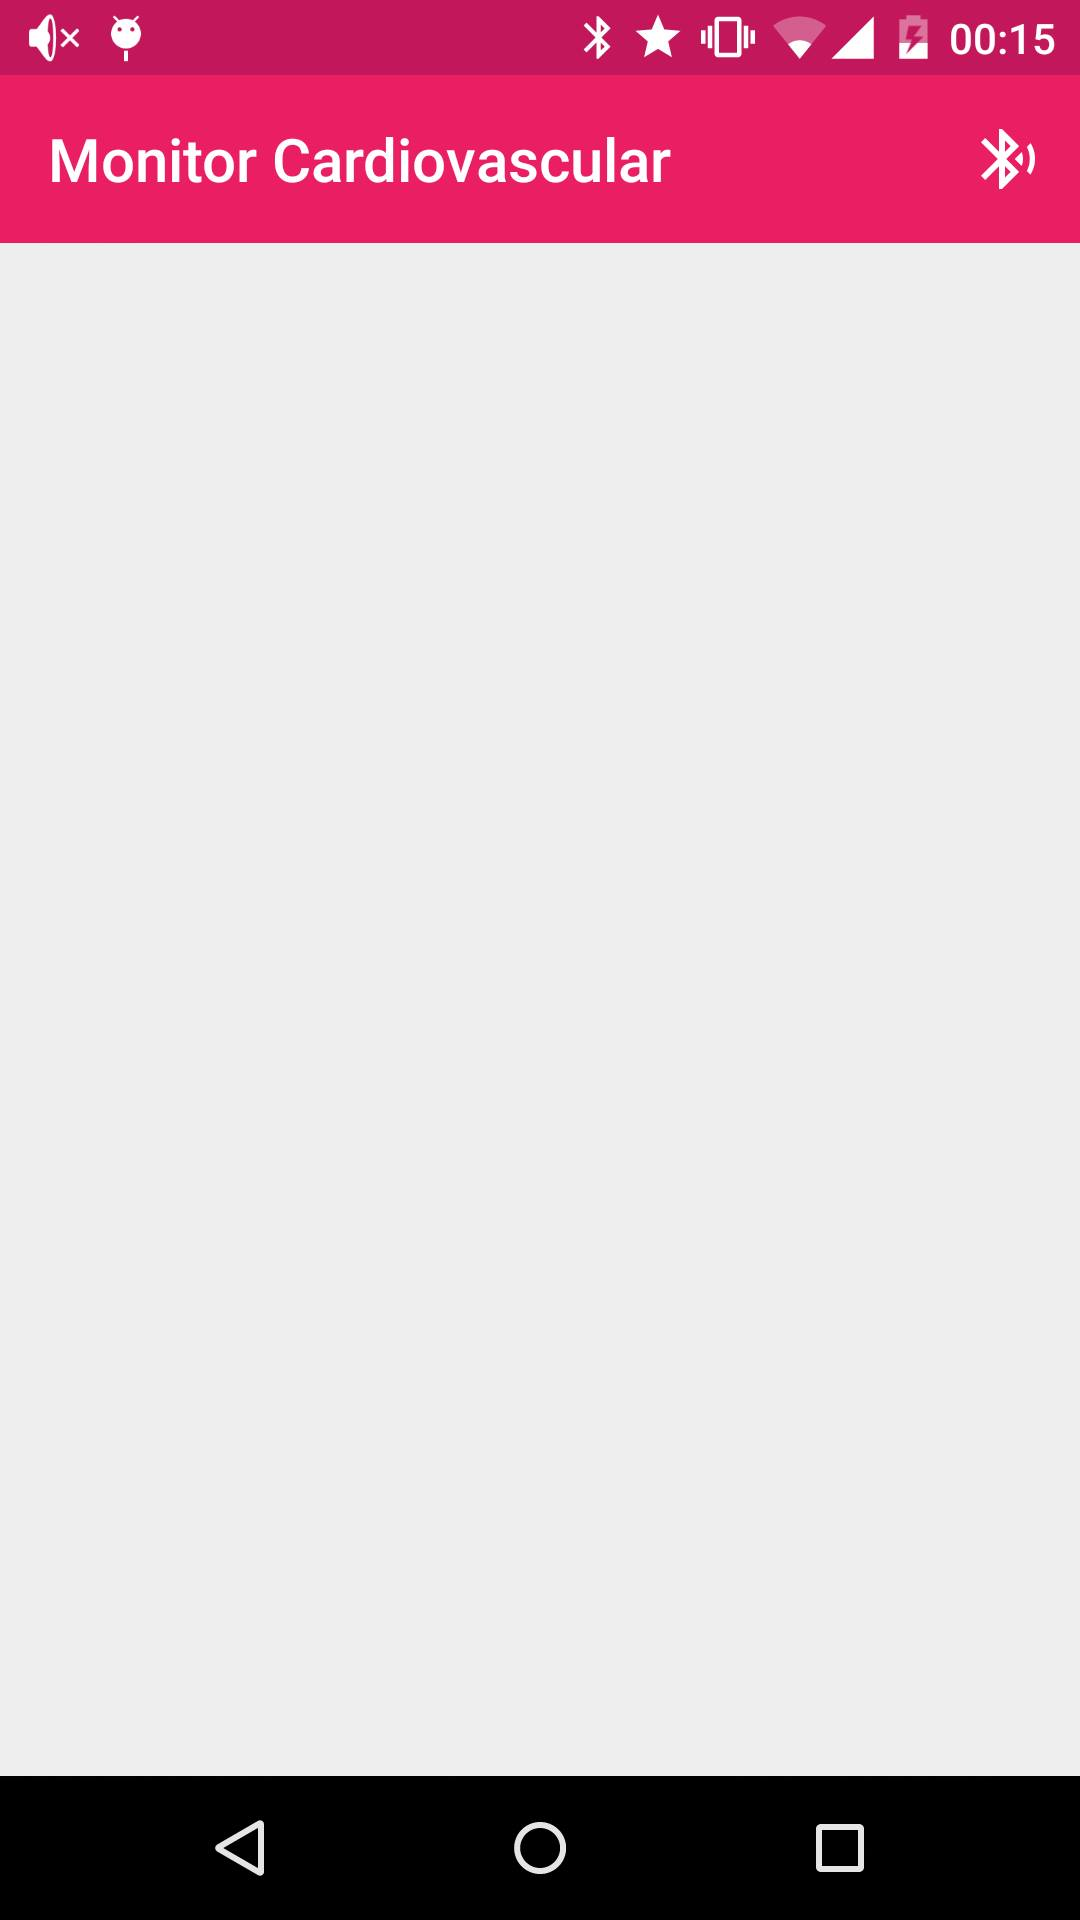
\includegraphics[height=11cm]{graphs/AndroidInicial.png} \caption{Pantalla inicial}\label{fig:screen:initialState}
\end{minipage}
\hfill
 \begin{minipage}{0.45\textwidth}\centering
    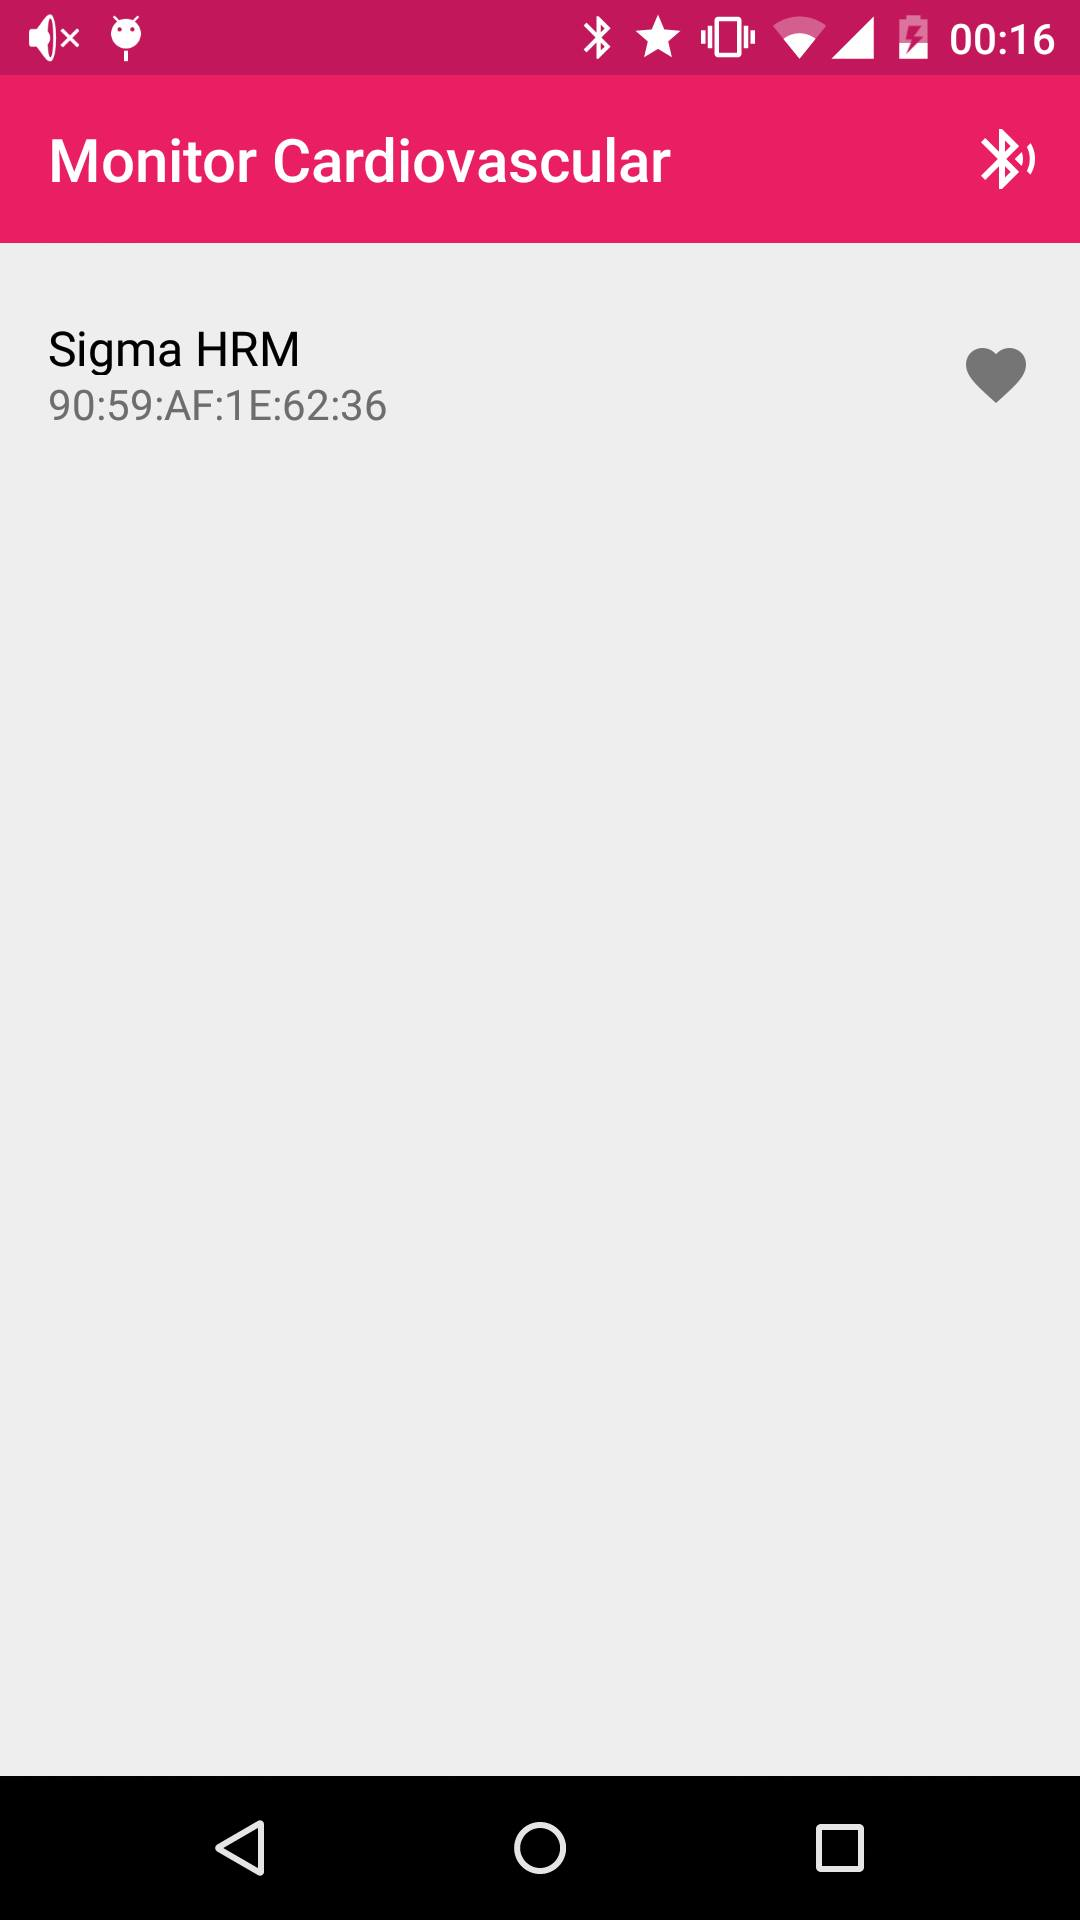
\includegraphics[height=11cm]{graphs/AndroidEscaneo.png} \caption{Dispositivos encontrados}\label{fig:screen:scanning}
\end{minipage}
\end{figure}
    
   En este caso nos encontramos con dos servicios: el servicio ``Servicio Cardiovascular'', que presenta las características ``Medida del ritmo cardíaco'', ``Ubicación del sensor'' y ``Punto de control'' y el servicio ``Servicio de batería'', que presenta una característica que nos permite comprobar el porcentaje de batería restante del pulsómetro. Para empezar a recibir datos de frecuencia cardíaca debemos hacer click en la característica ``Medida del ritmo cardíaco''. Esto activará el cliente HTTP, de forma que enviaremos a nuestro servidor web cada valor que nos llega del pulsómetro. La interfaz de usuario también reflejará cada valor recibido en el campo ``Datos''. La figura \ref{fig:screen:Conectado} muestra dicho proceso.
 
 \begin{figure}[H] \centering
 \begin{minipage}{0.45\textwidth}\centering
    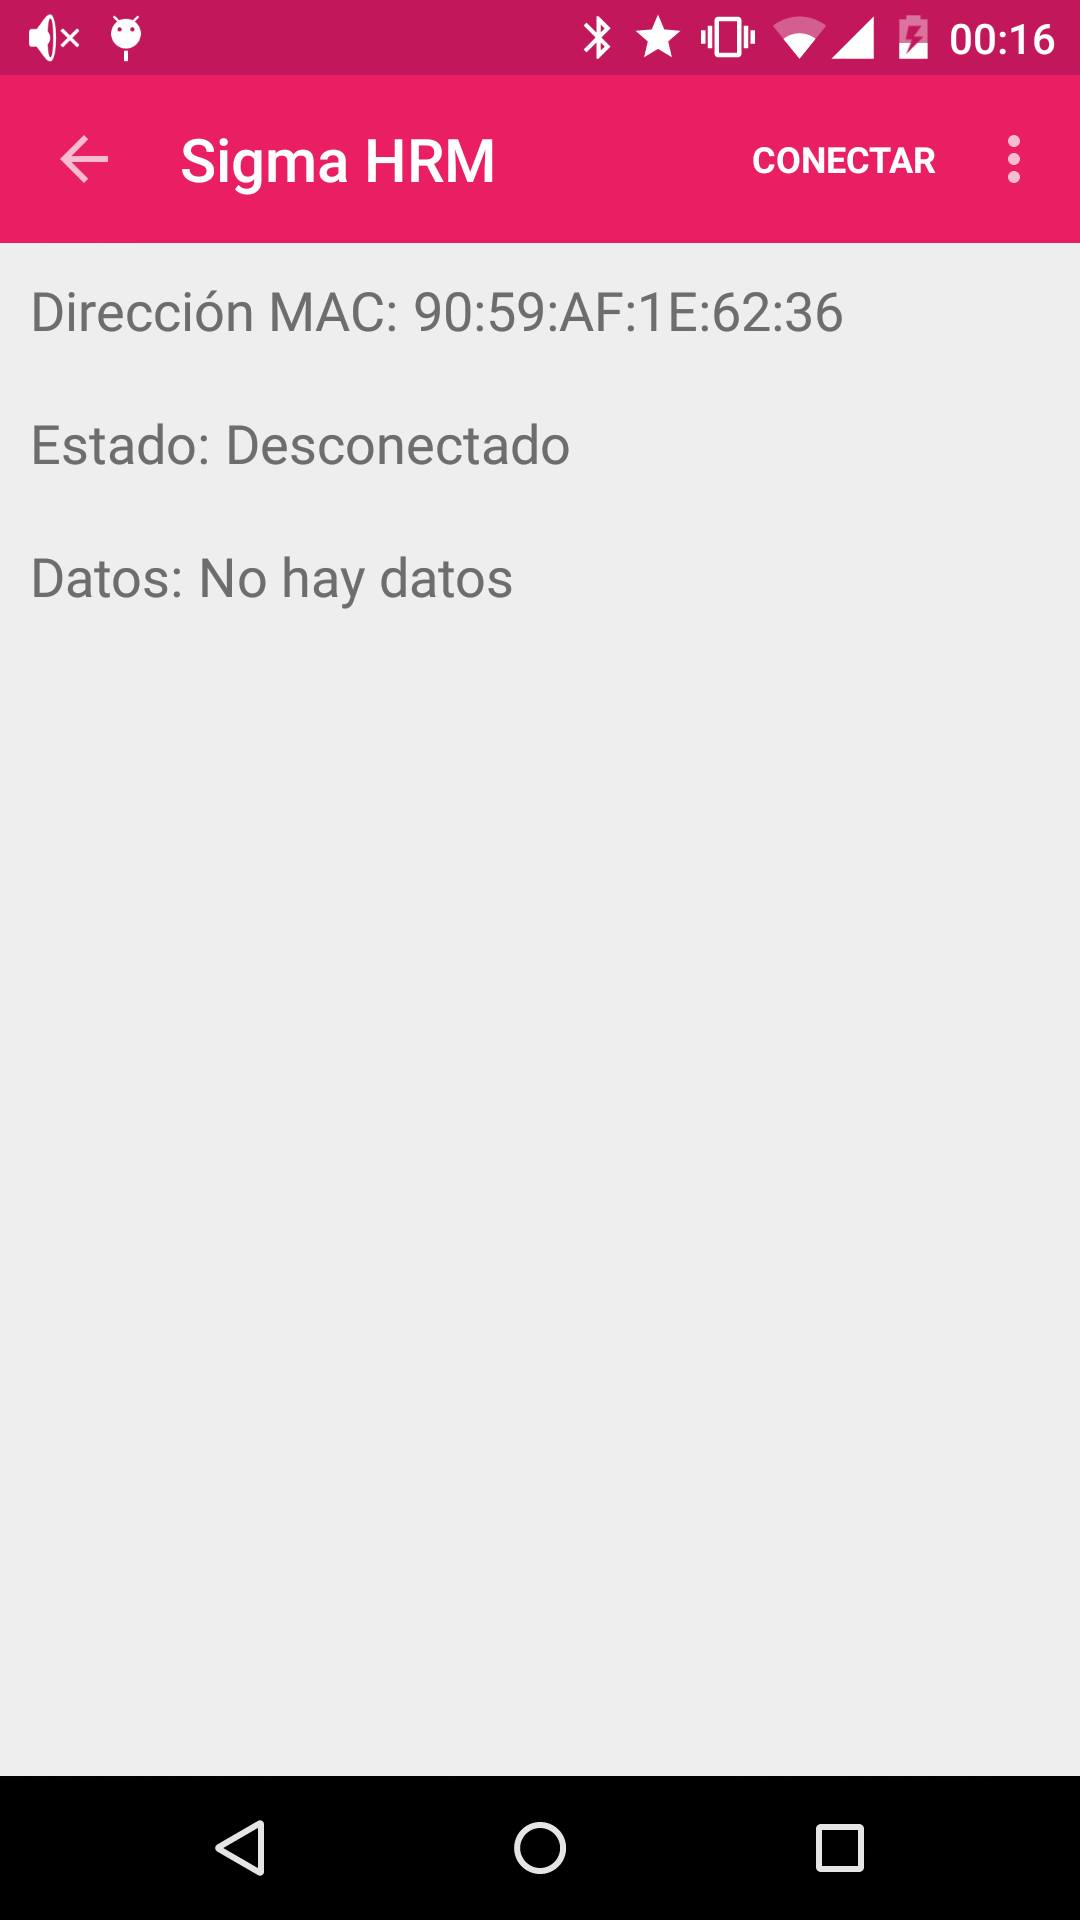
\includegraphics[height=11cm]{graphs/AndroidDesconectado.png} \caption{Conexión GATT sin establecer}\label{fig:screen:Desconectado}
 \end{minipage}
 \hfill
\begin{minipage}{0.45\textwidth}\centering
    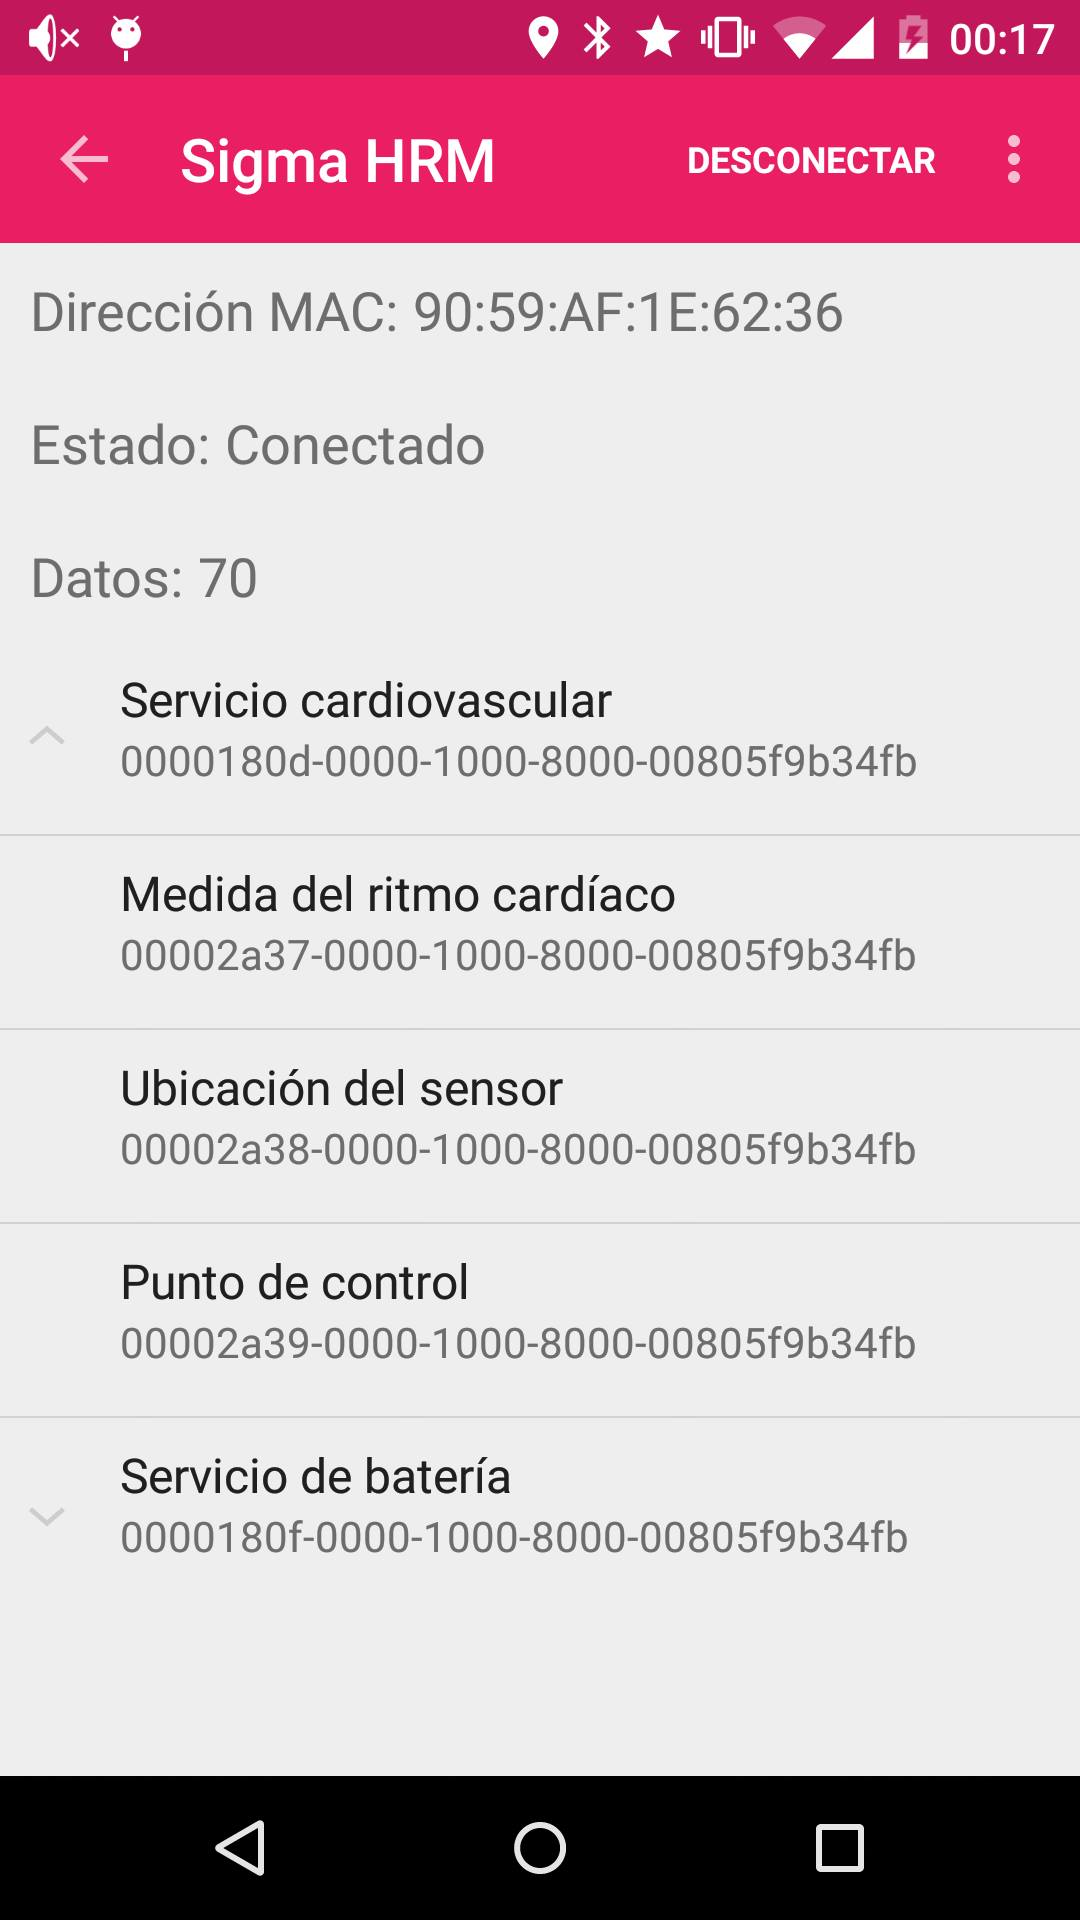
\includegraphics[height=11cm]{graphs/AndroidConectado.png} \caption{Conexión GATT establecida}\label{fig:screen:Conectado}
\end{minipage}
\end{figure}

Es importante mencionar que puesto la conexión GATT cliente-servidor es manejada mediante un servicio en segundo plano, podemos salir de la aplicación y realizar otras actividades, tales como abrir el navegador web o lanzar otras aplicaciones y esto no afectará al comportamiento de la aplicación.
Para desconectarnos del pulsómetro, solo debemos abrir la aplicación de nuevo y pulsar en el botón ``Desconectar''. Esto finalizará el servicio en segundo plano, la conexión GATT y hará que se liberen los recursos usados.

Mientras que estemos desconectados del pulsómetro, nuestro cliente web de monitorización mostrará el estado \tit{Desconectado} en todo momento, tal y como se observa en la figura \ref{fig:web:Desconectado}
    
\begin{figure}[h] \centering
	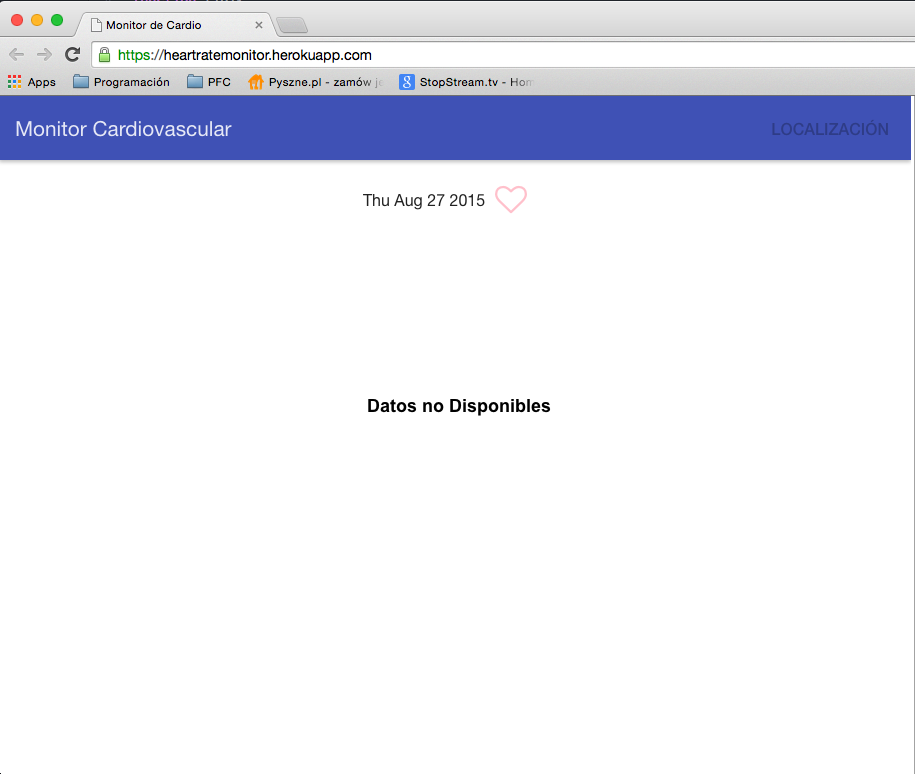
\includegraphics[width=15cm]{graphs/webDesconectado.png} \caption{Cliente web cuando el pulsómetro está desconectado}\label{fig:web:Desconectado}
\end{figure}

En cuanto conectamos con el pulsómetro y seleccionamos la característica de ``Medida del ritmo cardíaco'' en nuestra aplicación Android, los valores empiezan a llegar al servidor web, el cual establece una conexión permanente Web Socket con el cliente web, permitiendo una transmisión en tiempo real de dichos valores. La figura \ref{fig:web:Conectado} representa el cliente web en dicho estado.

\begin{figure}[h] \centering
	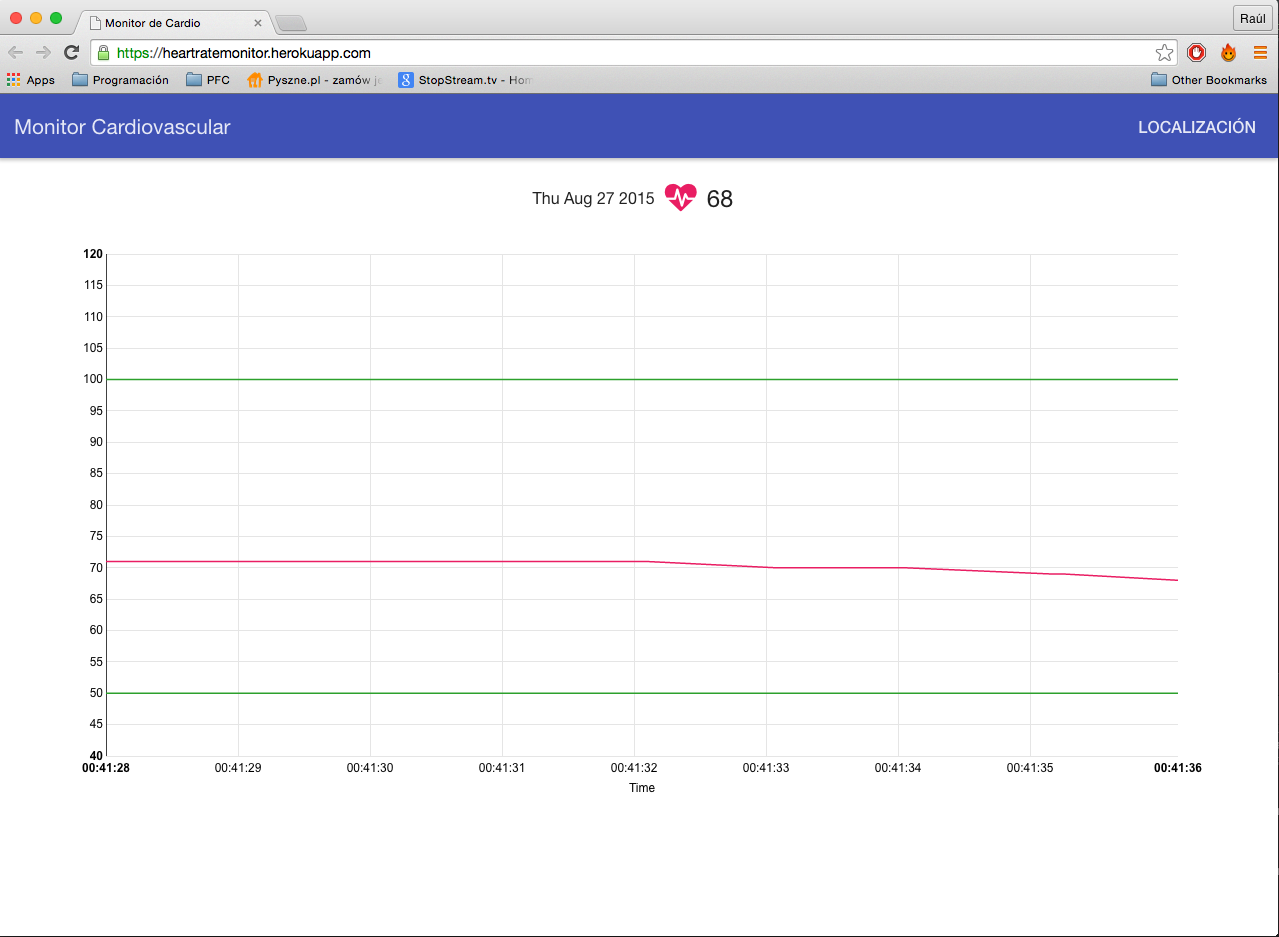
\includegraphics[width=15cm]{graphs/webConectado.png} \caption{Cliente web cuando el pulsómetro está conectado}\label{fig:web:Conectado}
\end{figure}

En la parte superior, justo debajo de la barra de navegación azul, se muestra la fecha actual, un icono representando la palpitación del corazón y el valor actual de frecuencia cardíaca recibido. Justo debajo aparece una gráfica en tiempo real mostrando el valor actual y los últimos valores recibidos con un trazo de color rosa. Las 2 lineas horizontales verdes, las cuales son fijas, delimitan un rango de valores estable (totalmente configurable en función del usuario a monitorizar). Esto está intrínsecamente relacionado con nuestro sistema de notificaciones, ya que se notificará por correo electrónico al usuario encargado de la monitorización siempre que nos topemos con valores fuera de rango, entrando en funcionamiento la lógica explicada en la sección \ref{cap:Servidor}, concretamente en la parte de notificaciones.

Esto se puede apreciar en las figuras \ref{fig:web:Notificaciones} y \ref{fig:web:Reposo}:

\begin{figure}[H] \centering
	\begin{minipage}{0.45\textwidth}\centering
		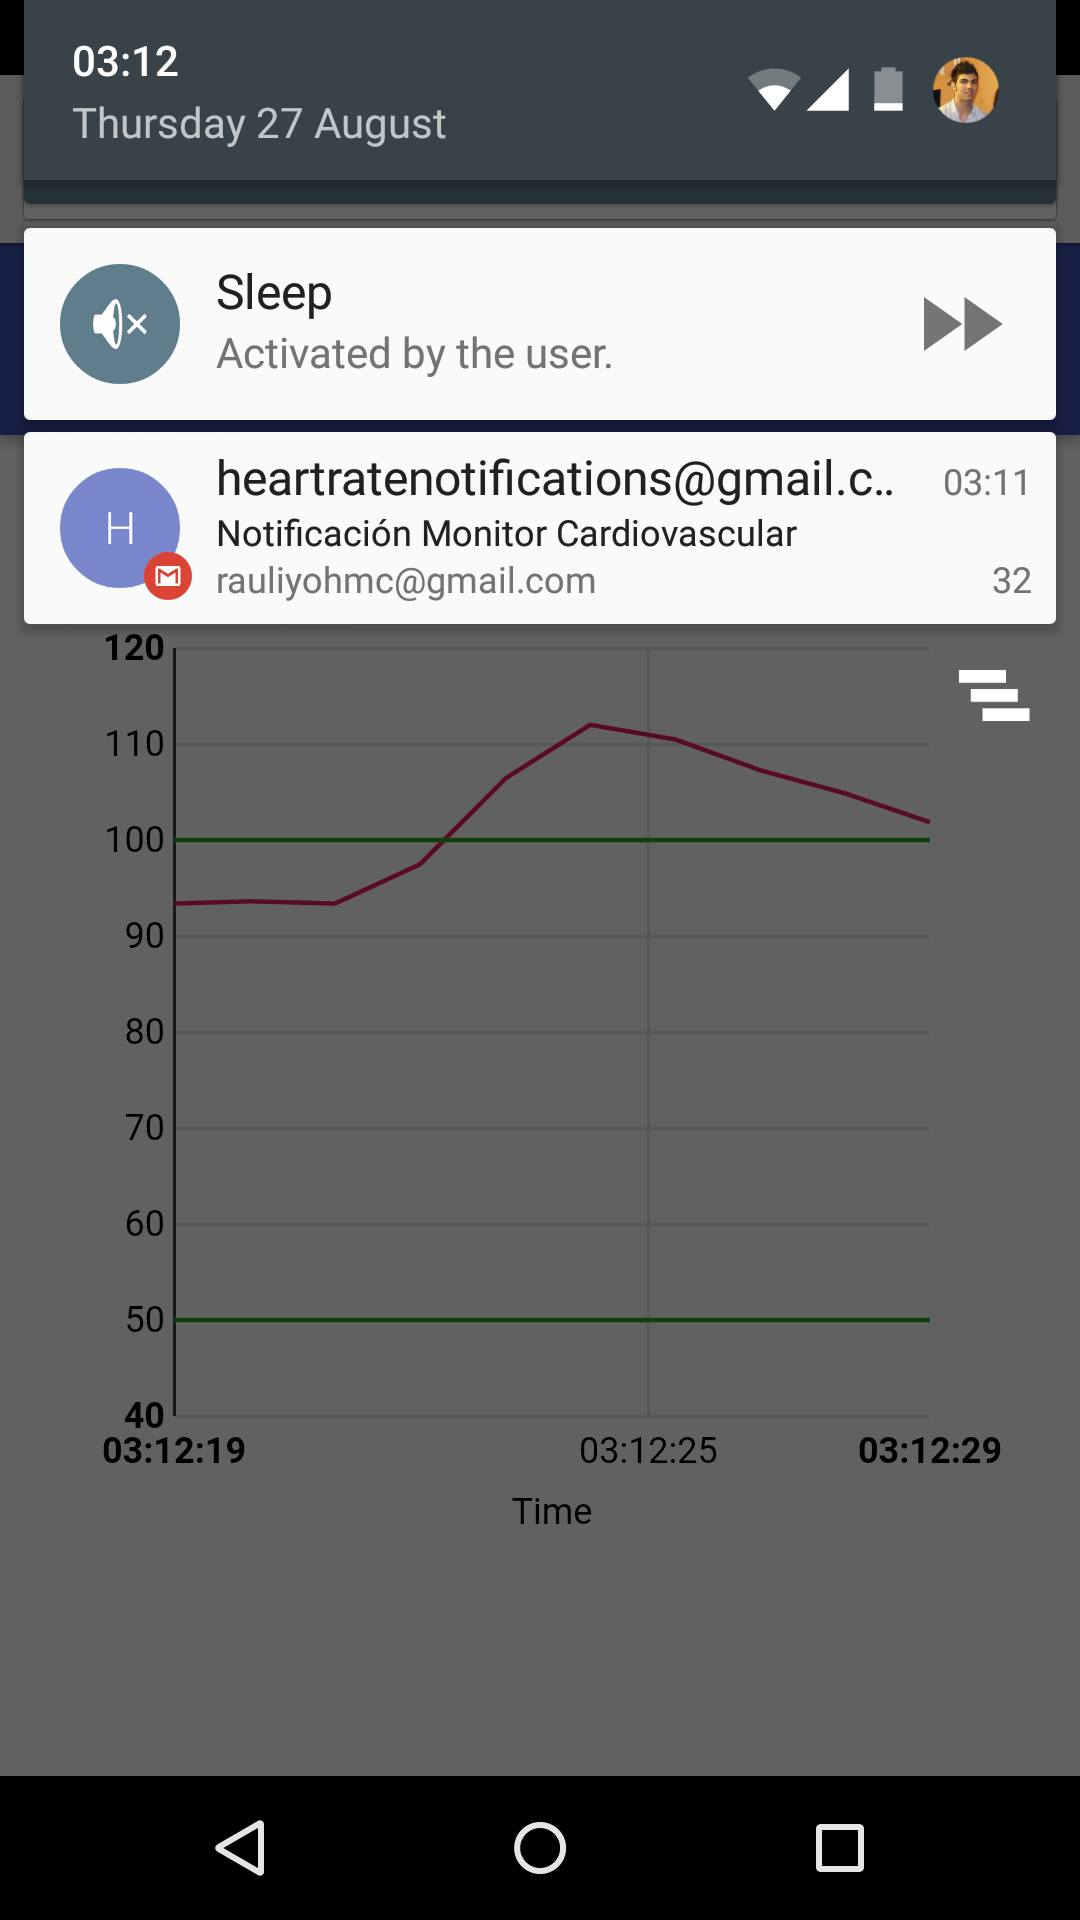
\includegraphics[height=11cm]{graphs/AndroidNotificaciones.png} \caption{Notificación por valor fuera de rango}\label{fig:web:Notificaciones}
	\end{minipage}
	\hfill
	\begin{minipage}{0.45\textwidth}\centering
		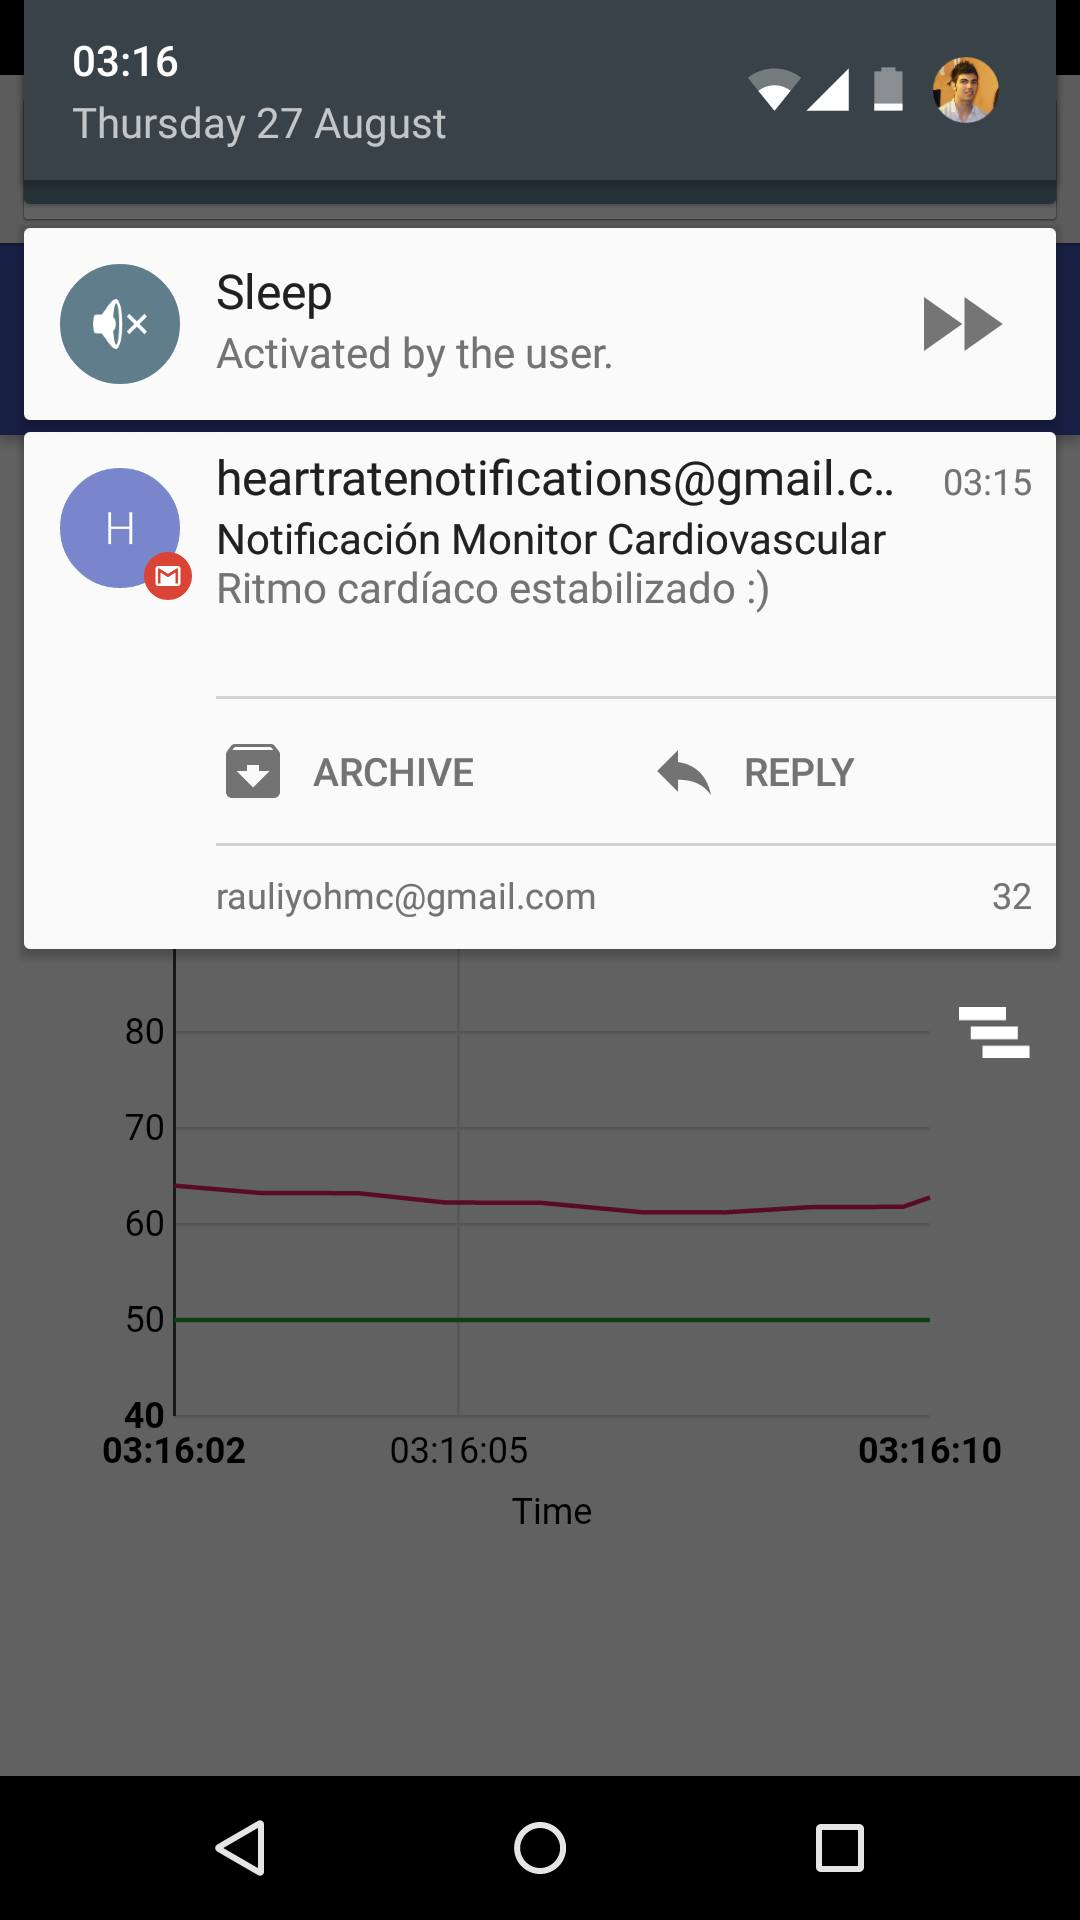
\includegraphics[height=11cm]{graphs/AndroidReposo.png} \caption{Notificación de estabilización}\label{fig:web:Reposo}
	\end{minipage}
\end{figure}

Para consultar la localización exacta del usuario en un determinado instante, debemos de pulsar el botón ``Localización''. Esto nos abrirá automáticamente la aplicación de Mapas de Google, determinando la localización en el mapa, así como la presentación de las coordenadas geográficas, como se puede ver en las figuras \ref{fig:web:Normal} y \ref{fig:web:Mapa}:

\begin{figure}[H] \centering
	\begin{minipage}{0.45\textwidth}\centering
		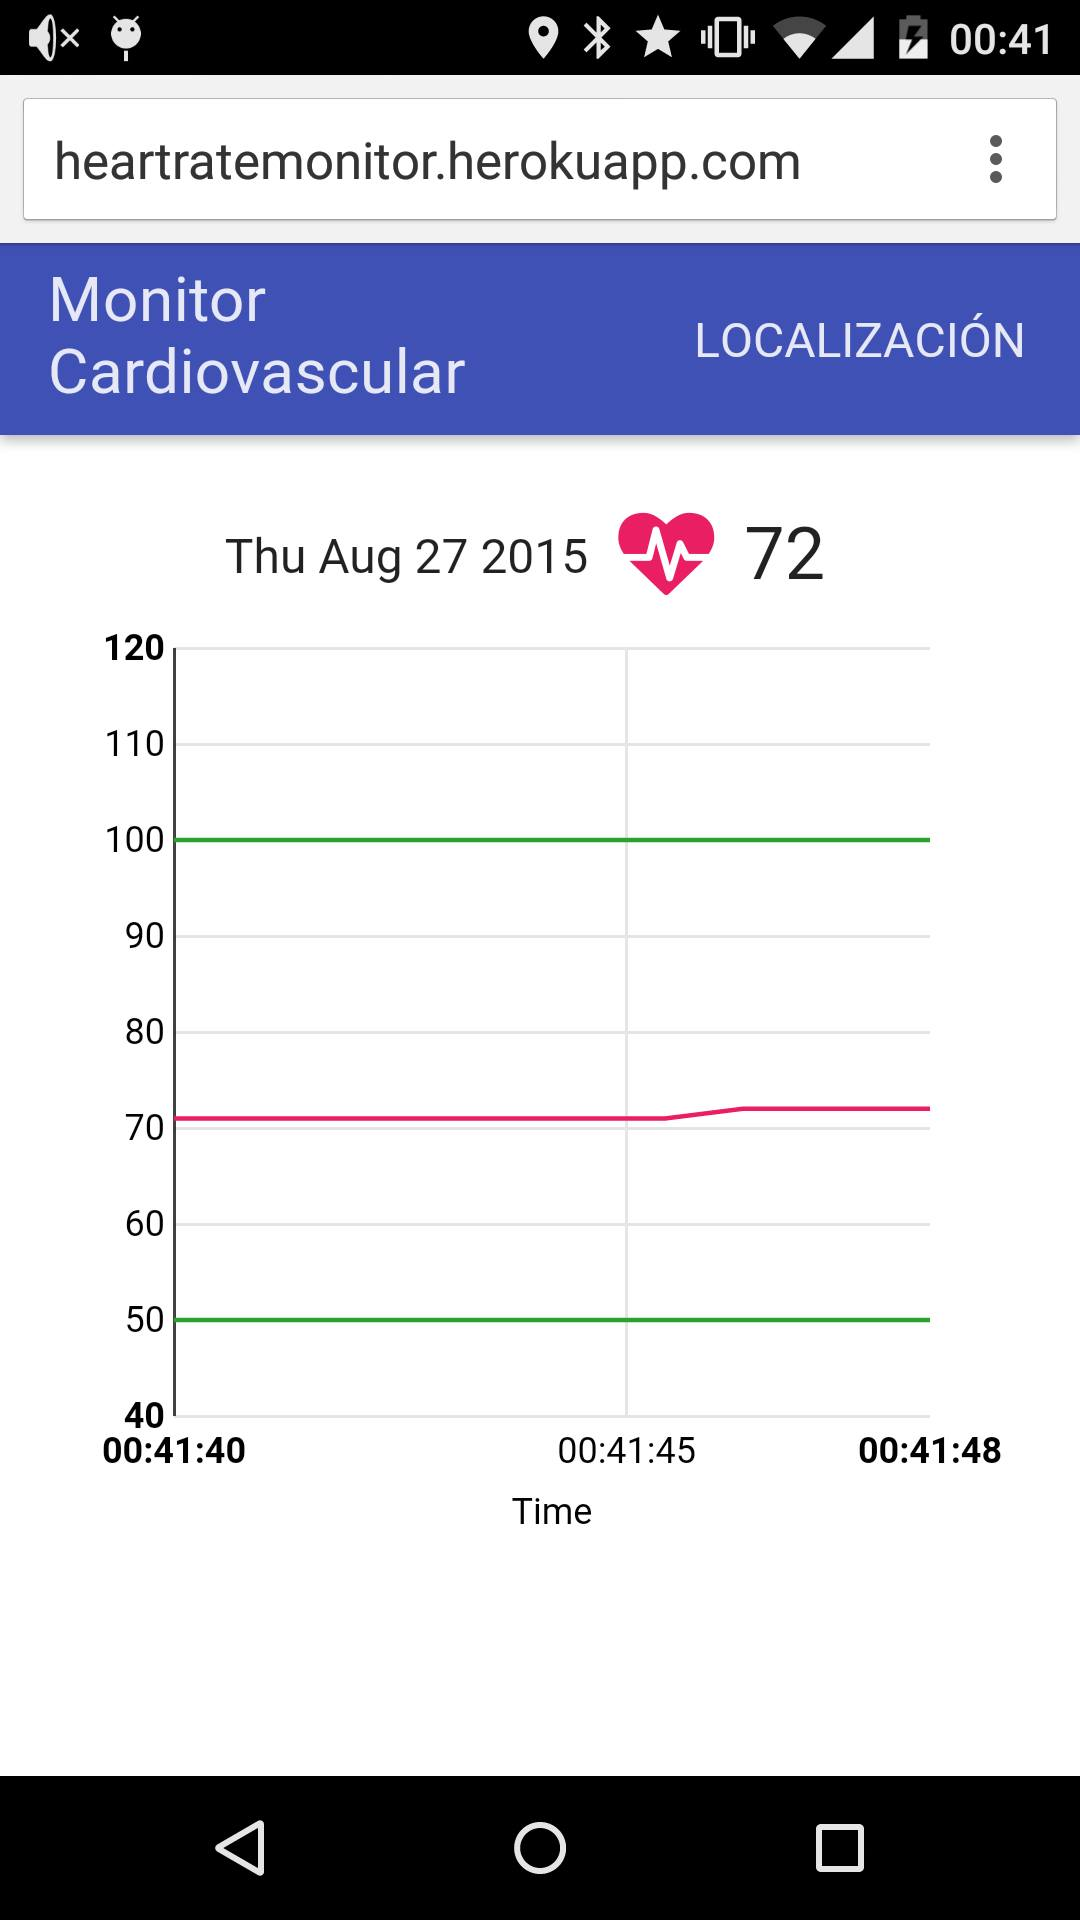
\includegraphics[height=11cm]{graphs/AndroidEmitiendo.png} \caption{Cliente web en un dispositivo móvil}\label{fig:web:Normal}
	\end{minipage}
	\hfill
	\begin{minipage}{0.45\textwidth}\centering
		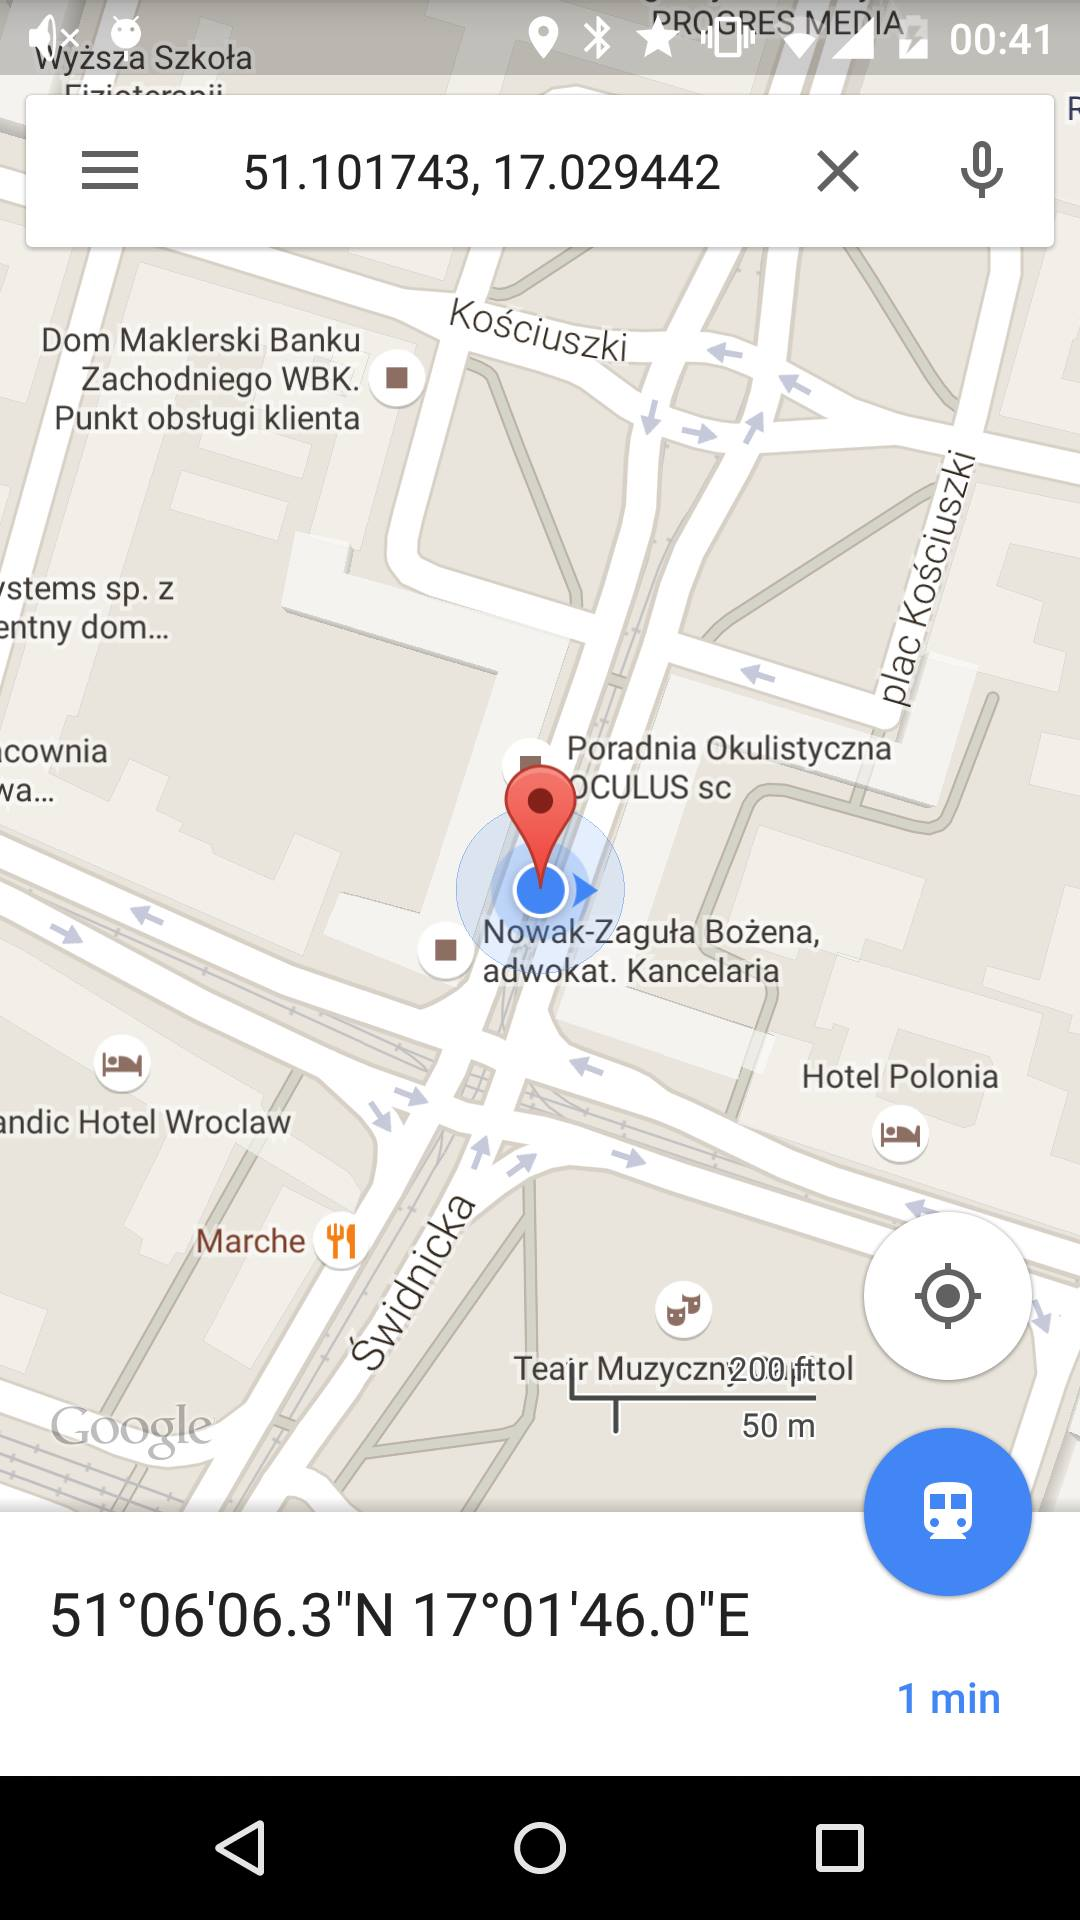
\includegraphics[height=11cm]{graphs/AndroidMapas.png} \caption{Ubicación del usuario en el servicio de mapas de Google}\label{fig:web:Mapa}
	\end{minipage}
\end{figure}

Por último y no menos importante, usamos una base de datos para registrar y guardar cada uno de los valores de frecuencia cardíaca que el servidor web recibe. Para ello hemos recurrido a Mongolab, un servicio de almacenamiento de datos en bases del tipo MongoDB en la nube, el cual nos proporciona de forma gratuita 512 MB de espacio.
La figura \ref{fig:web:dB} muestra un extracto de uno de los documentos almacenados, conteniendo muestras pertenecientes al momento Jueves 27 de Agosto, 3:13 a.m.

\begin{figure}[h] \centering
	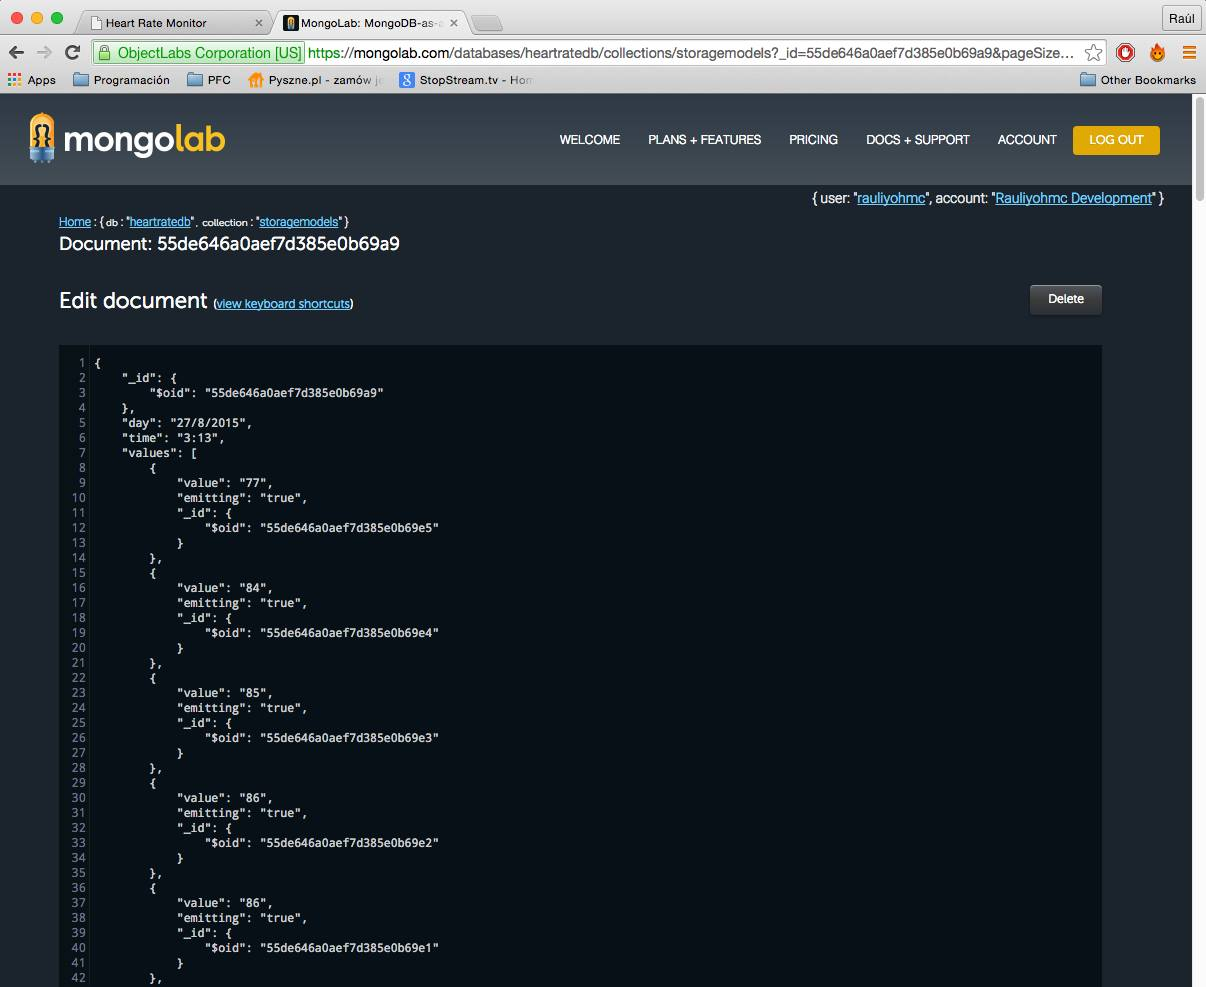
\includegraphics[width=15cm]{graphs/webDB.png} \caption{Servicio de almacenamiento MongoLab en la nube}\label{fig:web:dB}
\end{figure}

\section{Pruebas realizadas}
      
\subsection{Comparación con electrocardiograma}

\begin{figure}[h] \centering
	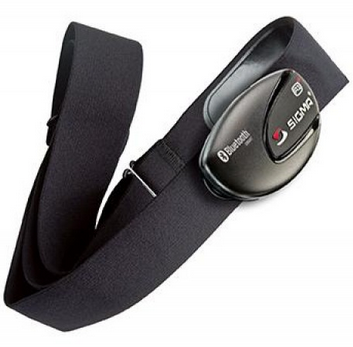
\includegraphics[width=10cm]{graphs/sigma.png} \caption{Sigma R1 Blue Comfortex+}\label{fig:sigma}
\end{figure}

Para cerciorarse de que los valores de frecuencia cardíaca mostrados en la aplicación se ajustan a la realidad, es necesario comparar los valores obtenidos por nuestro pulsómetro pectoral con un aparato de medición calibrado.
Para ello, recurrimos a la ayuda de una doctora ejerciendo en la ciudad de Wroclaw (Polonia), la cual amablemente se ofreció voluntaria para realizar medidas de nivel de frecuencia cardíaca emitidas por un electrocardiograma y así comparar los resultados con las medidas emitidas por el pulsómetro.

El pulsómetro utilizado ha sido el Sigma R1 Blue Comfortex+, el cual se muestra en la figura \ref{fig:sigma}. En el envoltorio podemos observar que afirma tener precisión de ECG (electrocardiograma).

Realizamos el estudio de 3 distintas situaciones, con todos los electrodos del electrocardiógrafo conectados a través del cuerpo y el pulsómetro Sigma comercial atado al pecho mediante su respectiva correa, con los dos electrodos situados en el pecho.
Los resultados obtenidos pueden verse reflejados en la tabla \ref{tab:SAR}:

\begin{table}[H]%
	\centering
	\begin{tabular}{|l|c|c|}
		\hline
		\hline
		\tbf{Actividad}&\tbf{Rango} &\tbf{Error (\%)}\\ \hline 
		\tbf{Reposo} &50-70 bpm& 5.8 \% \\ \hline
		\tbf{Actividad Ligera}& 80-100 bpm& 1.5 \% \\ \hline
		\tbf{Actividad intensa} &  150-170 bpm & 0 \% \\ \hline
		\hline 
	\end{tabular}
	\caption{Tabla de comparacion de mediciones} \label{tab:SAR}
\end{table}

En principio empezamos midiendo el latido del corazón en situación de reposo, mediante una posición estática estando de pie. Se pudo comprobar que existe una pequeña variación en la medida del pulsómetro relativa al electrocardiógrafo profesional, en torno a los +-3/4 bpm (latidos por minuto). Posteriormente empezamos una actividad cardiovascular ligera, alcanzando valores en el rango de las 80-100 pulsaciones por minuto y obtuvimos una mayor precisión, en torno a los +-1/2 bpm. Por último realizamos un trote intenso sobre el sitio hasta alcanzar valores cercanos a las 160 pulsaciones por minuto. De manera sorprendente, las medidas en este caso coincidían plenamente con las proporcionadas por el electrocardiograma.

Concluimos pues con unas medidas bastante exactas en todos los casos, llegando a igualar la medición del electrocardiograma en situaciones de ejercicio intenso. Esto se debe a que, en esencia, el fundamento del pulsómetro comercial de pecho es el mismo que el del electrocardiograma, registrando la actividad eléctrica del corazón que se produce en cada latido cardíaco.

Como contrapartida, existen sensores ópticos del ritmo cardíaco, los cuales funcionan mediante la emisión de luz LED a los capilares, y midiendo la frecuencia de bombeo de la sangre. Estos proveen una precisión alta en situaciones de reposo e inmovilidad, pero no son capaces de medir la frecuencia cardíaca en movimiento. Y en situaciones en las que paramos a medir el latido del corazón después de un intenso ejercicio proveen una precisión bastante baja, con errores en la medida de hasta el 40 \%.

\subsection{Consumo de energía}
Hemos realizado una estimación del consumo de batería medio que nuestra aplicación Android exige. Para ello, hemos usado el dispositivo conectado y emitiendo al servidor durante una hora en reposo, y durante una hora haciendo ejercicio en el exterior. El teléfono móvil utilizado ha sido un Nexus 5.
Durante el periodo en reposo, utilizando conexión inalámbrica a Internet, el teléfono disminuyó su batería un 5 \% en una hora, lo que nos da una estimación de duración de unas 20 horas, siempre que no usemos otras aplicaciones, ya que aquí solo consideramos el consumo del servicio funcionando en segundo plano.
Durante el periodo de ejercicio, y usando la red LTE de un plan de pago, la batería bajó en un 12 \% en una hora, lo que nos da una duración aproximada de 8.5 horas.

Los resultados obtenidos son sorprendentes y nos brindan un sistema capaz de aguantar medio día sin tener que recargar la batería, todo ello considerando todos los recursos utilizados mientras el servicio funciona en segundo plano, que son ni más ni menos el servicio de localización de Google, la conexión GATT cliente-servidor y los envíos de datos al servidor web a través del protocolo HTTP. Este bajo consumo se ve justificado por el hecho de que el protocolo BLE consume muy poca energía. La poca carga de datos que las peticiones HTTP acarrean y el alto intervalo de escaneo del servicio de localización (comprobando cada 2 minutos si existe una nueva posición del usuario) también contribuyen a dicho propósito.

\subsection{Retardo del sistema}
Cuando hablamos de retardo del sistema, nos referimos al tiempo que ha pasado desde que recibimos una nueva muestra de frecuencia cardíaca en nuestra aplicación puente Android, hasta que dicho valor aparece reflejado en la aplicación web. Obviamente esto está influenciado en parte por la velocidad de conexión a Internet en la cual nos encontremos sumergidos. En cualquier caso hoy en día las conexiones que manejamos a diario, ya sea en casa usando una conexión ADSL de alta velocidad, o nos encontremos en la calle usando una conexión HDSPA o LTE proporcionada por el proveedor de servicios contratado nos garantizan un rápido acceso a Internet.

\begin{figure}[h] \centering
	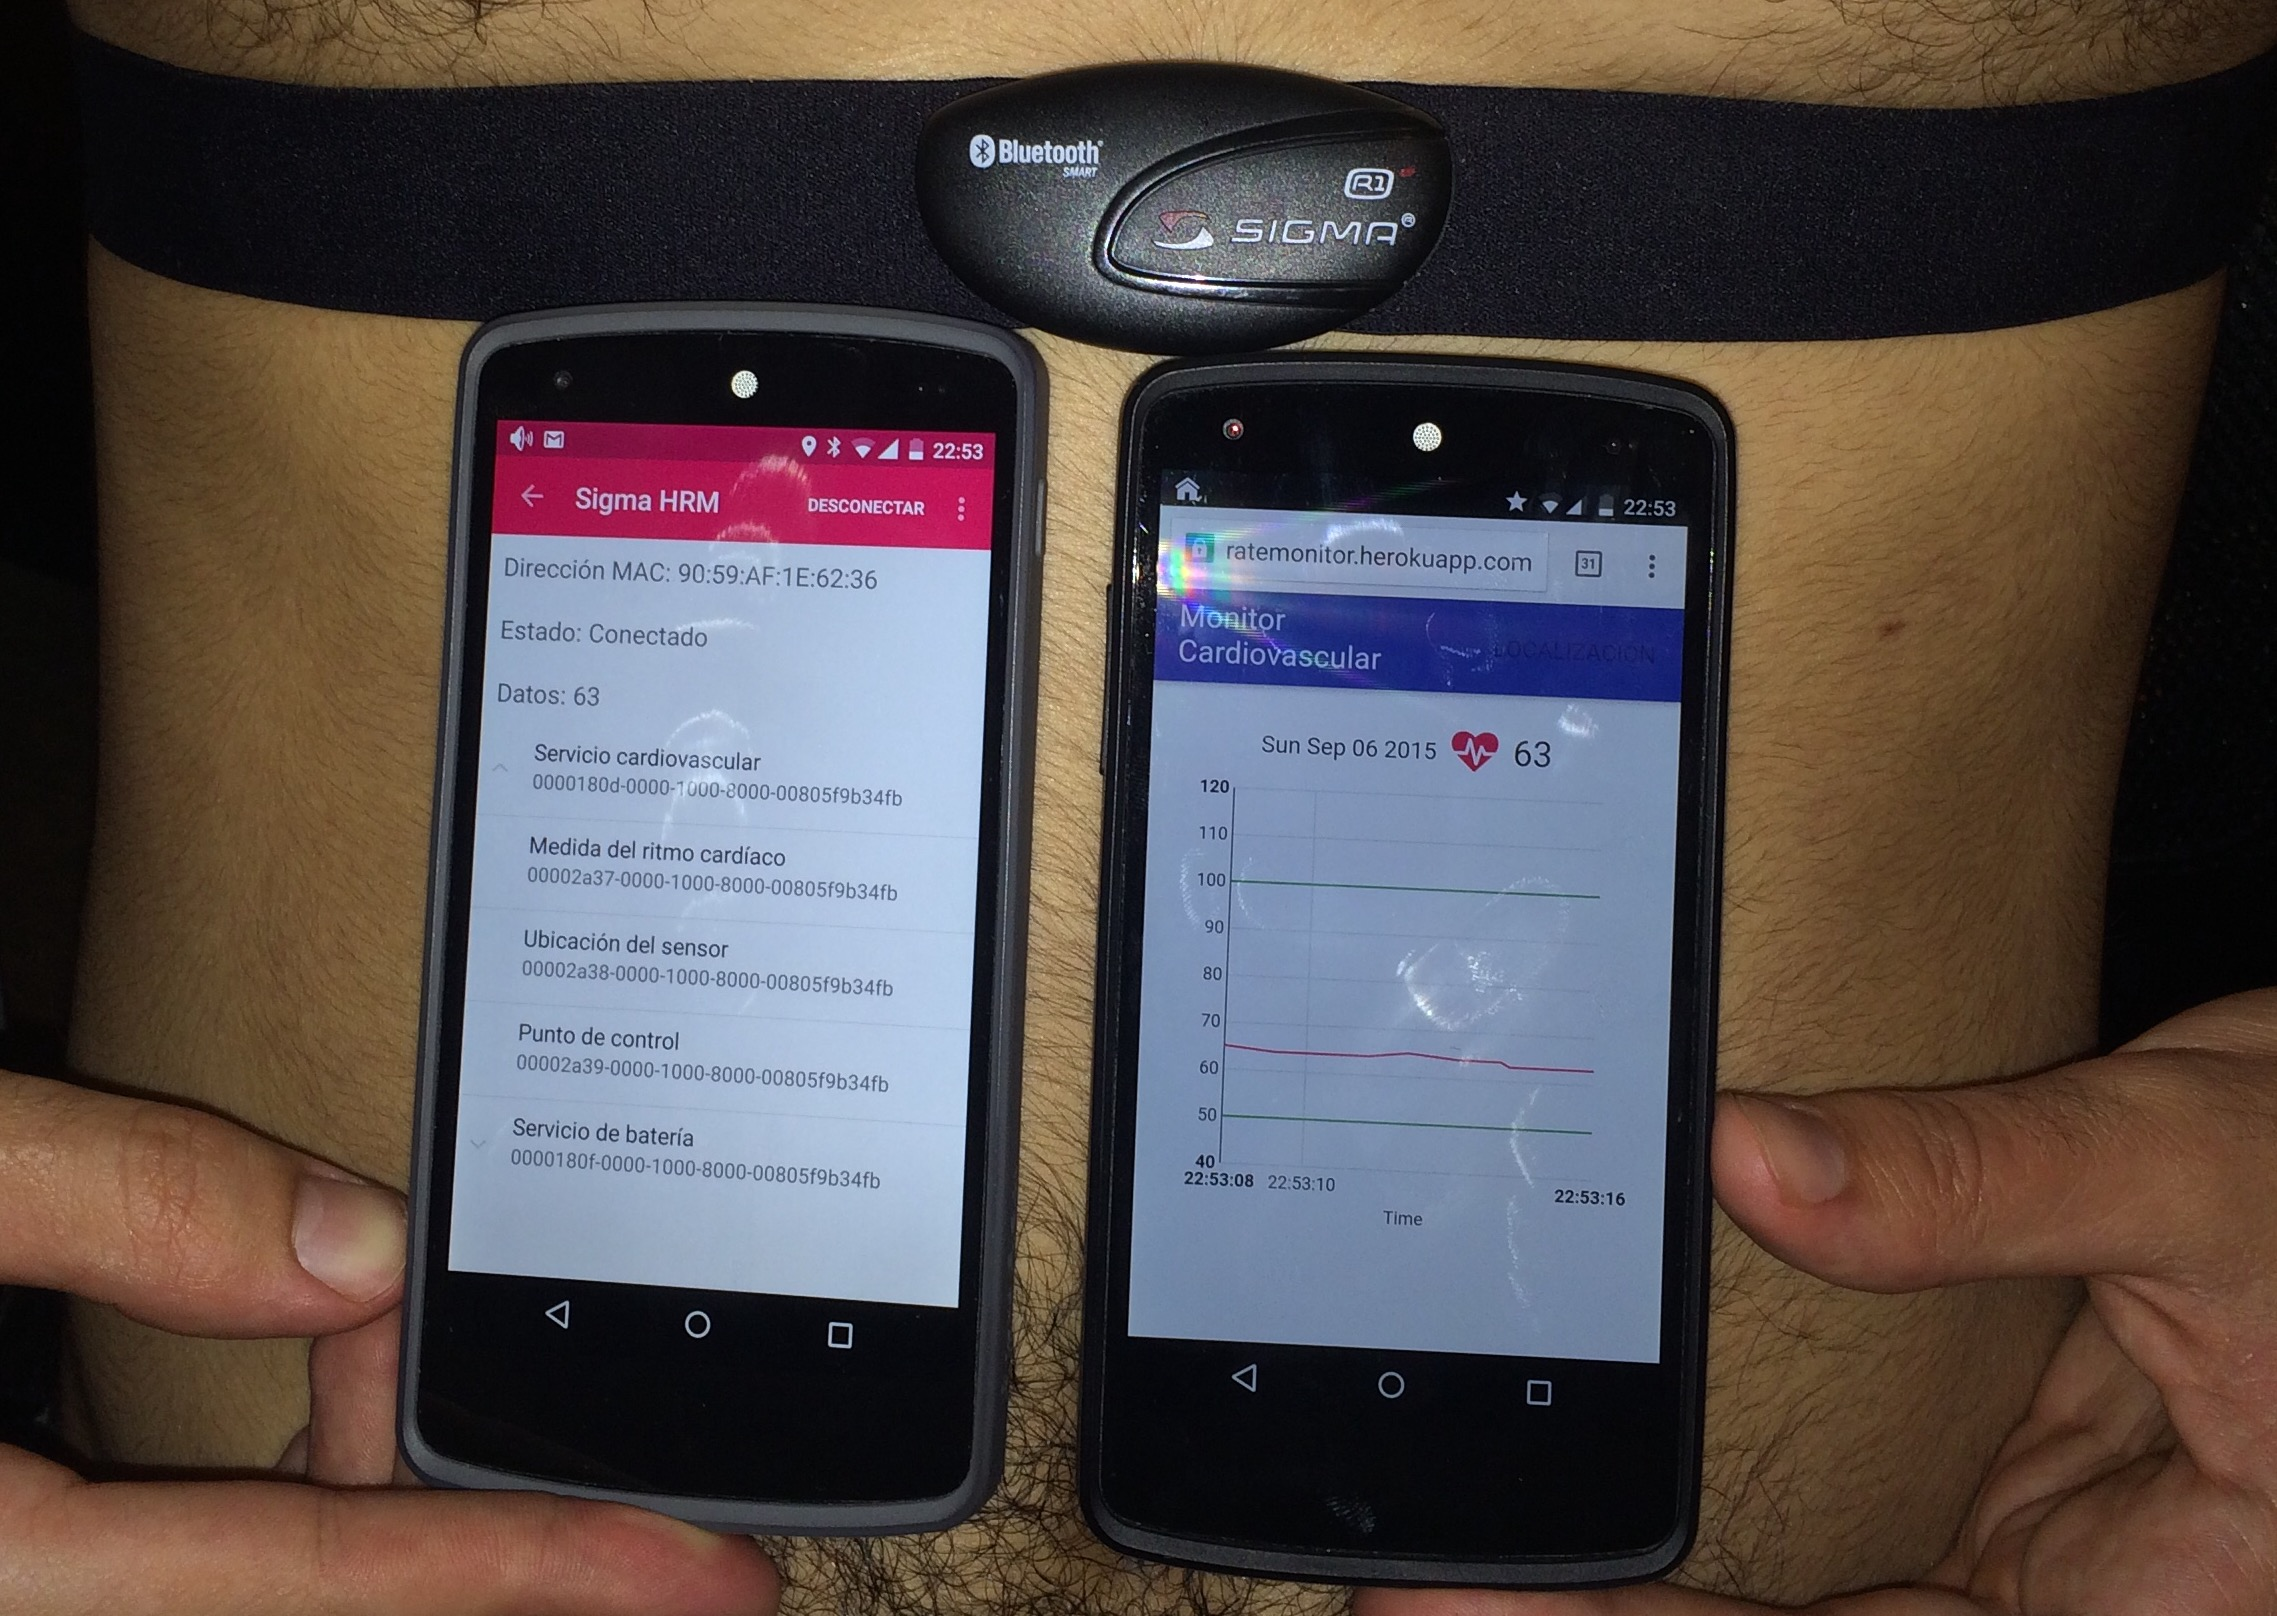
\includegraphics[width=15cm, keepaspectratio]{graphs/FullSizeRender.png} \caption{Captura del sistema en funcionamiento}\label{fig:prueba}
\end{figure}

Hemos puesto nuestro sistema a prueba en el caso extremo para estudiar su viabilidad. Para ello hemos recurrido a Heroku, un servicio gratuito de almacenamiento de aplicaciones web en la nube. El servidor que se nos ha asignado se encuentra en Virginia, Estados Unidos, con lo cual vamos a experimentar una conexión Wroclaw-Virginia-Wroclaw. El primer paso se trata de enviar los datos desde nuestra aplicación Android a nuestro servidor web localizado en Estados Unidos y posteriormente el servidor deberá entregar dichos datos a nuestro navegador web mediante la emisión de eventos utilizando una conexión de tipo socket.

La figura \ref{fig:prueba} muestra una captura tomada durante la realización de la prueba. Como se observa, el móvil de la izquierda muestra la aplicación Android, que recibe la información del pulsómetro y la envía al servidor, mientras que el móvil de la derecha es el que muestra la información proporcionada por el servidor en el navegador web, pudiéndose ver como los valores de pulsación coinciden.

Los resultados son asombrosos, es prácticamente imposible apreciar un retraso desde que la aplicación Android muestra el valor recibido en el campo de datos, hasta que este se ve reflejado en la web. Podríamos estimar un retardo en torno a los 100 milisegundos siendo algo conservadores, con lo cual se cumple con creces el objetivo de simulación de tiempo real del sistema.

Para finalizar, hemos incluido un resumen de las pruebas realizadas en la figura \ref{table:pruebas}.

\begin{figure}[h] \centering
	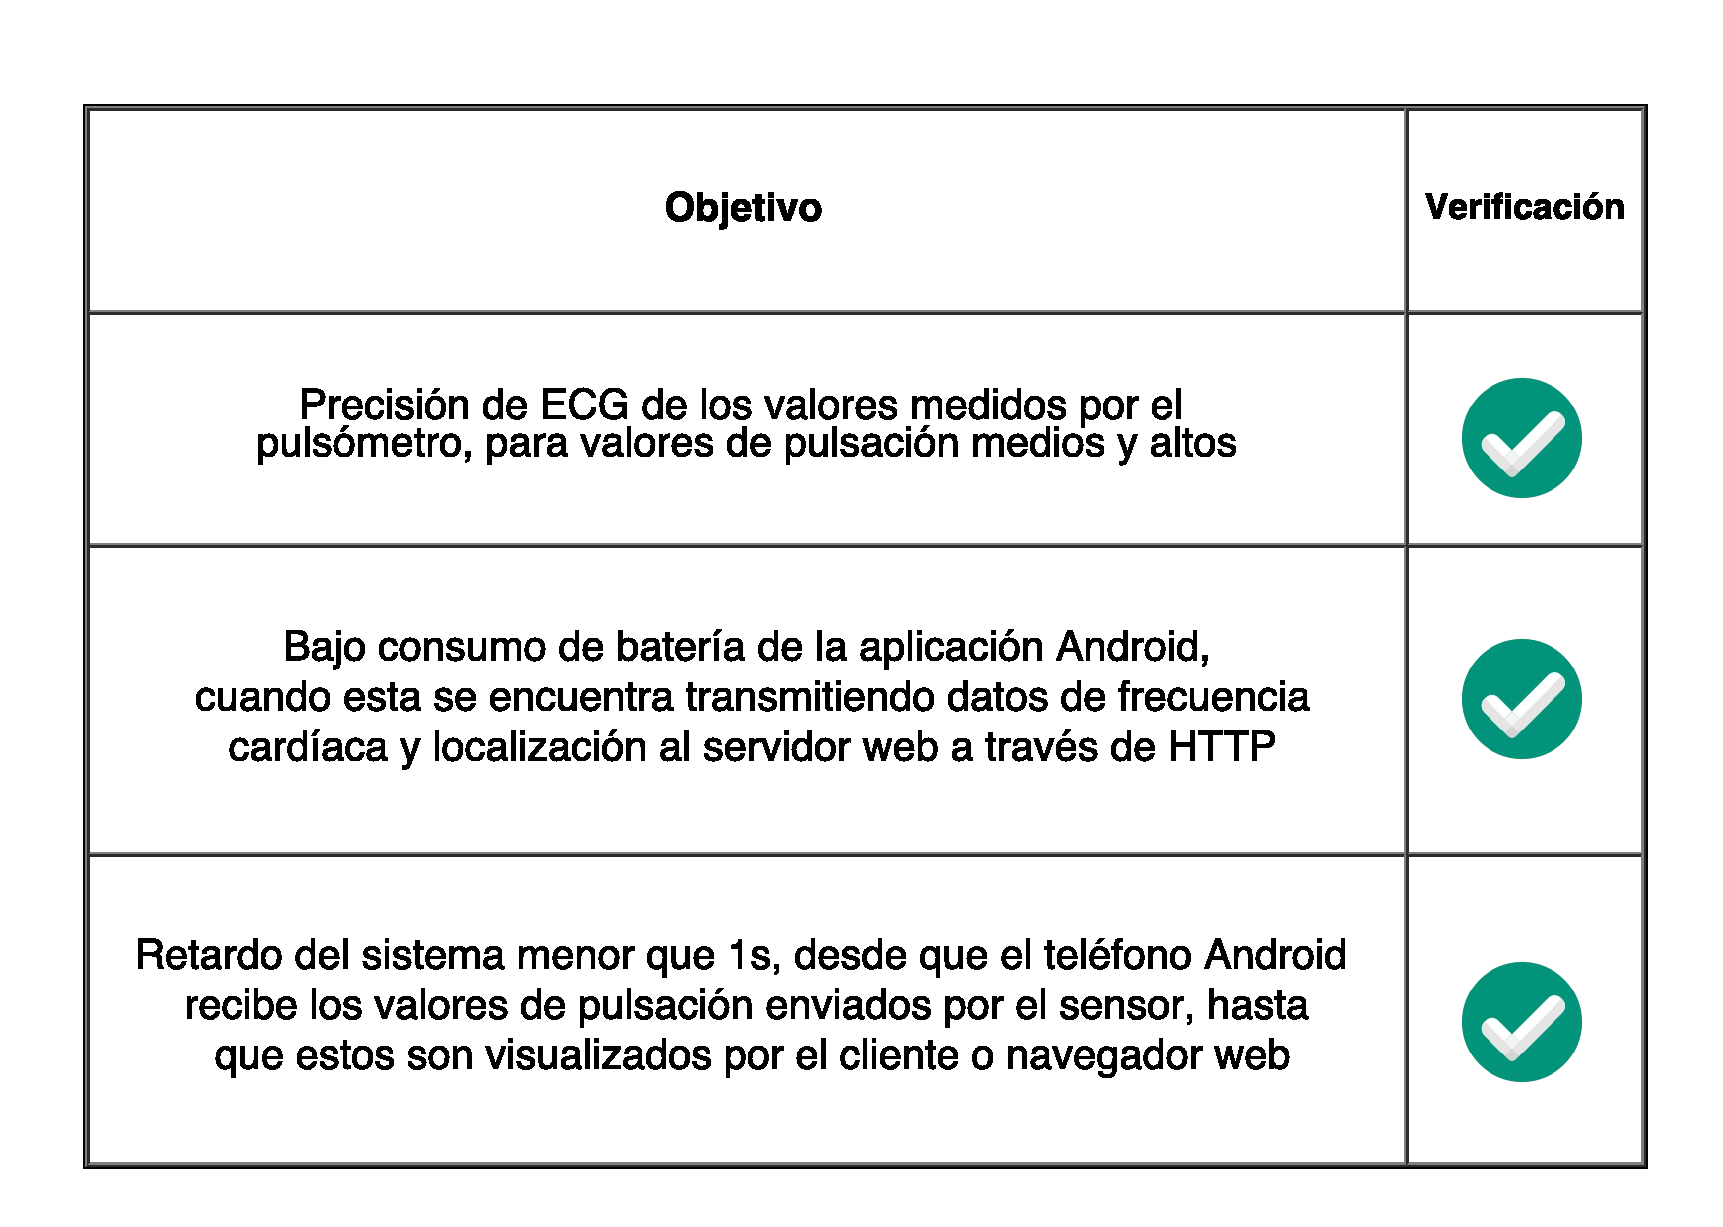
\includegraphics[width=15cm]{graphs/resumenObjetivos.pdf} \caption{Resumen de las pruebas realizadas}
	\label{table:pruebas}
\end{figure}
 
\section{Realización de los objetivos}

\subsection{Aplicación Android}

\subsubsection{Capacidad de detectar sensores BLE próximos al dispositivo}
    La aplicación cumple con el objetivo de ser capaz de escanear sensores con pila de reloj que usan el protocolo BLE para emitir información, ya sean monitores de frecuencia cardíaca u otra orientación médica, emisores de publicidad, etcétera.

\subsubsection{Capacidad de conectarse a cualquier sensor BLE registrado}
    La aplicación permite conectarnos a cualquiera de ellos para así consultar los servicios GATT ofrecidos, junto con cada una de sus características GATT, tal y como se observa en la figura \ref{fig:screen:Conectado}.

\subsubsection{Capacidad de leer características GATT ofrecidas por el sensor}
    La aplicación es capaz de leer el valor contenido en una cierta característica GATT, mediante la interpretación interna de sus descriptores, proporcionando un valor legible para el ser humano, como puede ser el valor de frecuencia cardíaca (mostrado en el campo ``datos'' de la figura \ref{fig:screen:Conectado}), la posición del sensor en el cuerpo, o el porcentaje de batería restante del sensor.
    
\subsubsection{Capacidad de enviar los parámetros relevantes a través del protocolo HTTP a nuestro servidor web}
   La aplicación cumple con el objetivo de enviar al servidor web los valores de ritmo cardíaco y localización obtenidos a través de los servicios que corren en segundo plano.
    
\subsection{Aplicación web}

\subsubsection{Capacidad de determinar si el sensor está conectado al sistema}
	La aplicación cumple con el objetivo de reflejar en todo momento el estado de la conexión del sensor. El estado desconectado se manifiesta mediante la iconografía de un corazón hueco y mediante la ausencia de gráfica en el centro de la pantalla, tal y como se aprecia en la figura \ref{fig:web:Desconectado}. El estado conectado se representa mediante la iconografía de un corazón palpitando.
	
\subsubsection{Capacidad de mostrar la frecuencia cardíaca actual en tiempo real}
	La aplicación es capaz de mostrar el valor de frecuencia cardíaca en tiempo real, mediante la indicación numérica justo a la derecha del icono de corazón latiendo, tal y como se aprecia en la figura \ref{fig:web:Conectado}.
	
\subsubsection{Capacidad de mostrar la evolución de la frecuencia cardíaca mediante el uso de una gráfica dinámica}
	La aplicación cumple con el objetivo de dibujar los valores que van llegando en una gráfica dinámica, la cual mostrará el valor actual junto con los más recientes (cuyo número dependerá del tamaño de la pantalla). Esta gráfica simula un comportamiento en tiempo real, desplazando valores a la izquierda conforme nuevos valores llegan. También presenta dos trazos horizontales configurables representando unos posibles límites dañinos o peligrosos.

\subsubsection{Capacidad de guardar los datos de frecuencia cardíaca en una base de datos}
	La aplicación es capaz de guardar en una base de datos todo registro de frecuencia cardíaca recibido, ordenándolos en documentos de 60 muestras cada uno, representando aproximadamente un minuto de actividad. Esto permitirá un fácil acceso o consulta mediante la indicación del minuto exacto como clave de acceso, así como el día en cuestión.
	
\subsubsection{Capacidad de determinar la posición del usuario usando el servicio de mapas de Google}
	La aplicación cumple con el objetivo de ser capaz de determinar la posición absoluta del dispositivo móvil, gracias al servicio de mapas de Google, tal y como se puede observar en la figura \ref{fig:web:Mapa}. El punto azul representa dicha posición.
	
\subsubsection{Capacidad de notificar por e-mail a un grupo de usuarios interesados en realizar tareas de monitorización}
	La aplicación cumple con las expectativas de notificar al usuario en caso de valores fuera de rango, mediante el envío instantáneo de correos electrónicos, los cuales informarán en todo momento de la evolución de la situación hasta que se detecte una estabilización de los valores, lo que conllevará el fin del periodo de notificaciones a través de una notificación final informativa. En dichos correos también se adjuntará la localización del usuario. Esto se ve reflejado en las figuras \ref{fig:web:Notificaciones} y \ref{fig:web:Reposo}.

\subsubsection{Capacidad de adaptarse fácilmente a pantallas más pequeñas, tales como teléfonos móviles y tabletas}
	La aplicación cumple con el objetivo de adaptarse también a dispositivos móviles, los cuales presentan pantallas más pequeñas, siendo capaz de mostrar información con la misma calidad que si nos encontrásemos en un ordenador personal, sin forzar al usuario a enfocar la pantalla mediante un aumento. Esto se aprecia perfectamente en la figura \ref{fig:web:Reposo}.
	
\chapterend{}

\part{Conclusiones y líneas futuras}
\chapterbeginx{Conclusiones y líneas de trabajo futuras}
\label{chp:concl}
\sectionx{Conclusiones}
    
    En este proyecto se ha investigado, planificado y desarrollado un sistema, presentado como una combinación de dos aplicaciones Android y web funcionando como un todo, cuyo objetivo es la monitorización de parámetros del sistema cardiovascular, en particular el ritmo cardíaco, todo ello buscando una conexión en tiempo real que presente el menor retardo posible.
    
    Durante el proyecto se han tenido en cuenta los conocimientos adquiridos durante el estudio de la titulación de Ingeniero de Telecomunicación, en particular aquellos relacionados con arquitectura de computadores y programación. Debido a que Comunicaciones fue la especialidad elegida en el último curso, se ha optado por usar e integrar uno de los protocolos de comunicaciones de última generación como es el protocolo Bluetooth 4.0, en concreto su modo de baja energía, una de las novedades que ha permitido la comercialización de millones de sensores de bajo coste y consumo.
    
    Uno de los mayores retos del proyecto ha sido las implementaciones de ambas aplicaciones Android y web. Durante la titulación no se han cursado asignaturas relativas a programación móvil, Java o programación web. Habiendo desarrollado algo de código Java por cuenta propia, el factor de mayor novedad y en el que más se ha aprendido durante la realización del proyecto es el componente web del mismo, gracias a la implementación del servidor, base de datos, y cliente web, es decir, todo el stack completo usando Javascript. Este valioso conjunto de conocimientos sienta las bases para, en un futuro, poder construir aplicaciones web de mayor complejidad técnica.
    
    La aplicación generada como resultado de este Proyecto Fin de Carrera, responde de manera satisfactoria a los objetivos autoimpuestos al principio del mismo, tal y como se ha demostrado en el capítulo de pruebas. Por tanto, al haber obtenido un producto funcional, se considera el proyecto como exitoso.
    
\sectionx{Líneas de trabajo futuras}
    Durante el desarrollo del proyecto, y especialmente durante las pruebas finales del mismo, han surgido ideas y mejoras para el mismo, que son posibles de implementar en un futuro.
     
 \begin{description}
	\item[Aplicación Android cliente de monitorización] \hfill \\	
	Las aplicaciones como Facebook o Twitter presentan tanto versiones web como nativas para el sistema operativo Android. Los usuarios de teléfonos móviles descargan decenas de aplicaciones nativas y odian tener que abrir el navegador para acceder a una cierta aplicación, lo que les fuerza recordar la URL de la misma, accesos más lentos en caso de sobrecarga del servidor, etcétera. Mediante una aplicación Android cliente, mostraríamos la misma interfaz gráfica que presenta nuestra aplicación web, con la única diferencia que tenemos la aplicación nativa y fácilmente accesible, haciendo al cliente más feliz.
	
	\item[Guardar dispositivos preferidos]\hfill\\
	Consecuentemente ahorrando batería en nuestro teléfono Android. De esta forma antes de volver a escanear, intentamos en primer lugar conectar directamente al dispositivo.
	
	\item[Extension de los servicios GATT ofrecidos al servidor web]\hfill\\
	Dado que solo mandamos al servidor web datos de frecuencia cardíaca y localización, podríamos extender su funcionalidad mediante el envío de otras características GATT disponibles en el sensor, tales como la posición del sensor en el cuerpo, o mostrar el porcentaje de batería restante del sensor, para así prever con antelación un posible remplazo de la misma.
	
	\item[Reconocimiento de actividad]\hfill \\	
	Android incorpora una API, conectada a los servicios de localización de Google, que permite estimar la actividad física realizada por el usuario con una probabilidad bastante alta. De esta forma podríamos mandar dicha información al servidor web para así ser capaces de monitorizar también la actividad actual del usuario y ver si este se encuentra corriendo, pedaleando una bicicleta, o sentado, entre otras muchas posibilidades.
	
	\item[Extensión a relojes con sistema operativo Android]\hfill\\
	Con la reciente aparición de Android wear, podríamos desarrollar la aplicación compatible con este tipo de dispositivos, con lo cual la aplicación sería mucho más portable, al no depender de nuestro teléfono móvil. El hecho de que la aplicación funciona la mayoría del tiempo en segundo plano justifica la viabilidad de dicha extensión.
	
    \item[Inclusión de gráficas estadísticas]\hfill \\	
    Mediante la consulta de valores de ritmo cardíaco almacenados en la base de datos, podríamos construir en nuestra aplicación web gráficas tales como históricos, evoluciones diarias, o en cualquier otro caso obtener valores mediante el procesado de dichos datos, tales como la frecuencia cardíaca media, intervalos RR, máximos y mínimos, etcétera, los cuales pueden ser de gran utilidad a analistas especializados.
    
    \item[Sistema de autentificación]\hfill \\
    Se podrían crear perfiles personalizados para cada usuario individual, configurando parámetros como rango de valores peligrosos, o correo electrónico a notificar. Para ello dotaríamos a nuestra página web de un sistema de registro y autentificación, haciendo uso de la base de datos. De esta forma solo el personal autorizado tendría acceso a los datos y estadísticos oportunos proporcionando privacidad a los clientes, mediante el uso de las credenciales adecuadas (usuario y contraseña).
    
    \item[Exportación de archivos]\hfill\\
    Posibilidad de exportar gráficas y estadísticos mediante el pulsado de un botón, facilitando el compartir los datos con otros analistas que puedan presentar interés en la información.
    
    
\end{description}

\begin{flushright}
{\large \pfcauthorname}\nli
\today
\end{flushright}
	
\chapterend{}

% Anexos
\part{Apéndices}

\appendix

%%%%%%%%%%%%%%%%%%%%%%%%%%%%%%%%%%%%%%%%%%%%%%%%%%%%%%%%%%%%%%%%%%%
%%% Documento LaTeX 																						%%%
%%%%%%%%%%%%%%%%%%%%%%%%%%%%%%%%%%%%%%%%%%%%%%%%%%%%%%%%%%%%%%%%%%%
% Título:		Apéndice A
% Autor:  	Ignacio Moreno Doblas
% Fecha:  	2014-02-01
% Versión:	0.5.0
%%%%%%%%%%%%%%%%%%%%%%%%%%%%%%%%%%%%%%%%%%%%%%%%%%%%%%%%%%%%%%%%%%%%

\pagestyle{fancy}
\fancyhead[LE,RO]{\thepage}
\fancyhead[RE]{Apéndice} %
\fancyhead[LO]{\nouppercase{\rightmark}}
%\fancyhead[RE]{Parte \thepart \rightmark} %
\chapterbegin{Proceso de integración de una aplicación node.js en Heroku}
   
   El proceso para integrar nuestra aplicación node.js en cualquiera de los servidores dedicados ofrecidos por el servicio Heroku es bastante sencillo. Asumiendo que nos hemos registrado satisfactoriamente con nuestro correo electrónico, en primer lugar debemos instalar el cinturón de herramientas Heroku, el cual puede ser accedido a través del enlace
   
   \mbox{\url{https://devcenter.heroku.com/articles/getting-started-with-nodejs}}.
    
   Este nos brinda acceso a la interfaz de comandos Heroku mediante el terminal y nos proporciona un comando local ejecutable llamado \ttw{heroku}, el cual nos ayudará a la gestión de las aplicaciones de forma local.
   La figura \ref{fig:authentication} muestra el proceso de autentificación mediante el uso del comando \ttw{heroku login}

 \begin{figure}[H] \centering
    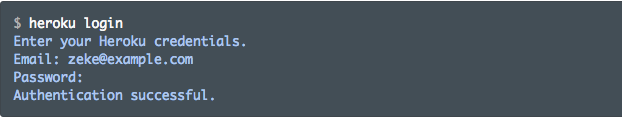
\includegraphics[width=15cm]{graphs/herokuLogin.png} \caption{Autentificación en el terminal en Heroku \cite{heroku}}\label{fig:authentication}
\end{figure}

Debemos tener en cuenta que si usamos un cortafuegos o firewall que requiere el uso de un proxy para conectarse con los servicios externos HTTP/HTTPS, tendremos que configurar las variables de entorno \ttw{HTTP\_PROXY} or \ttw{HTTPS\_PROXY} en nuestro entorno de desarrollo local previo a correr el comando.

El siguiente paso consiste en preparar la aplicación que queremos integrar en el servidor. Para ello nos situamos, localmente y desde el terminal, en el directorio el cual contiene nuestro archivo \ttw{package.json} con todas las dependencias. Debemos tener el código fuente enlazado y asociado a un repositorio git, como el proporcionado por el servicio Github por ejemplo. Ahora debemos ejecutar el comando \ttw{heroku create} para crear una aplicación en Heroku. Esto preparará a Heroku para que reciba nuestro código fuente. 

Cuando se crea la aplicación en Heroku, también se crea un repositorio remoto git llamado \ttw{heroku}, el cual estará asociado con nuestro repositorio local.

Heroku genera un nombre aleatorio para nuestra aplicación. Para asignar un nombre específico, lo pasamos como parámetro al comando. Esto se ve reflejado en la figura \ref{fig:deploy}

 \begin{figure}[H] \centering
    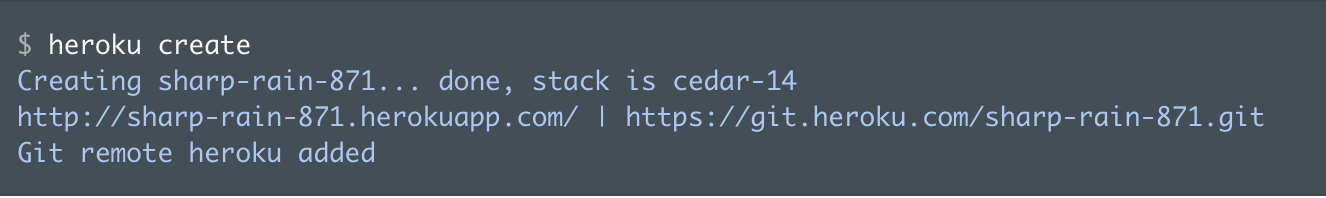
\includegraphics[width=15cm]{graphs/herokuDeploy.png} \caption{Preparando a Heroku para crear la aplicación \cite{heroku}}\label{fig:deploy}
\end{figure}

Ahora debemos enviar nuestro código fuente mediante el comando \ttw{git push heroku master}. El resultado se puede apreciar en la figura \ref{fig:push}.

 \begin{figure}[!htbp] \centering
    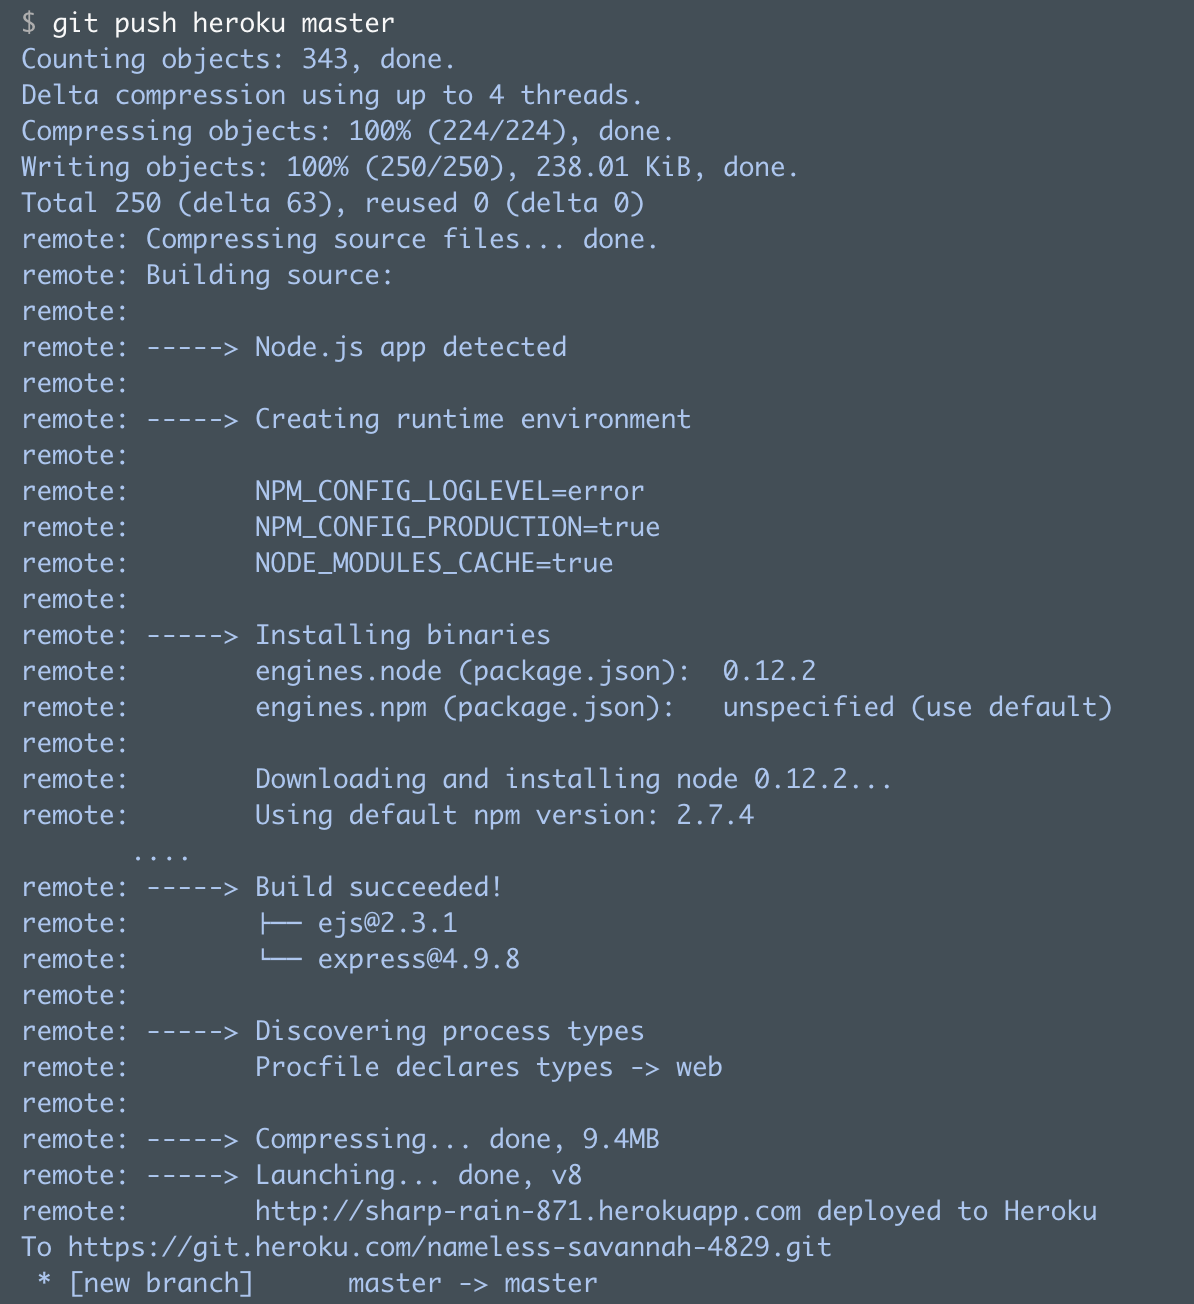
\includegraphics[width=15cm]{graphs/herokuPush.png} \caption{Enviando el código fuente a Heroku \cite{heroku}}\label{fig:push}
\end{figure}

La aplicación ya se encuentra desplegada en el servidor y podemos asegurarnos de que al menos una instancia de la aplicación está funcionando mediante el comando \ttw{heroku ps:scale web=1}.

Ahora ya podemos visitar la aplicación a través de la URL generada, en base al nombre pasado como parámetro (o el obtenido aleatoriamente). Independientemente, existe un comando útil para abrirla desde el terminal, \ttw{heroku open}.

Una vez que la aplicación se encuentra funcionando podremos consultar siempre que queramos los logs generados por Heroku y los nuestros personalizados en el código fuente a través del comando mostrado en la figura \ref{fig:logs}

 \begin{figure}[H] \centering
    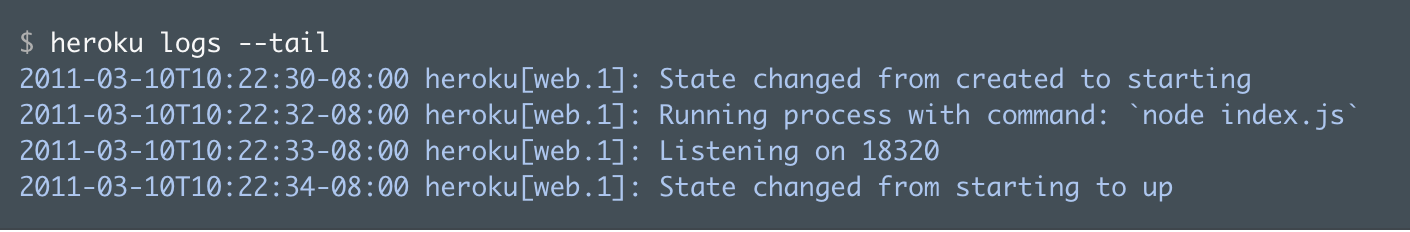
\includegraphics[width=15cm]{graphs/herokuLogs.png} \caption{Consulta de logs de nuestra aplicación \cite{heroku}}\label{fig:logs}
\end{figure}

Por último, mencionar que Heroku proporciona un Tablero de Instrumentos o Dashboard en su página web, desde el cual podremos monitorizar el estado de nuestra aplicación, controlar los permisos de acceso, configurar distintas opciones, consultar métricas específicas, etcétera. Algunas de las opciones son gratuitas y otras de pago. La interfaz presentada es la mostrada en la figura \ref{fig:dashboard}

 \begin{figure}[H] \centering
 	\includegraphics[width=15cm]{graphs/herokuDashboard.png} \caption{Apariencia del dashboard en Heroku \cite{heroku}}\label{fig:dashboard}
 \end{figure}

\chapterend

%\input{D2.AppendixB.tex}

%\input{D3.AppendixC.tex}

% Formato de documento en la parte final.
\backmatter
%Hace que los capítulos y títulos nivel inferior no aparezcan numerados (lo que es ideal para conclusiones o notas finales).

% Bibliografía
%%%%%%%%%%%%%%%%%%%%%%%%%%%%%%%%%%%%%%%%%%%%%%%%%%%%%%%%%%%%%%%%%%%
%%% Documento LaTeX 																						%%%
%%%%%%%%%%%%%%%%%%%%%%%%%%%%%%%%%%%%%%%%%%%%%%%%%%%%%%%%%%%%%%%%%%%
% Título:		Bibliografía
% Autor:  	Ignacio Moreno Doblas
% Fecha:  	2014-02-01
% Versión:	0.5.0
%%%%%%%%%%%%%%%%%%%%%%%%%%%%%%%%%%%%%%%%%%%%%%%%%%%%%%%%%%%%%%%%%%%%

% Encabezamiento %
\pagestyle{fancy}
\fancyhead[LE,RO]{\thepage}
\fancyhead[LO]{Bibliografía}
%\fancyhead[RE]{Parte \thepart \rightmark} %
\fancyhead[RE]{\nouppercase{\rightmark}} %

%Inclusión de bibliografía%
\bibliography{Bibliografia} %Úsese el nombre del fichero sin extensión

%Inclusión en el índice (Tabla de contenidos)
\addcontentsline{toc}{chapter}{Referencias}

%Formateo de estilo de bibliografía
% Otros formatos: plain, unsrt, abbrv
%  plain: las entradas se ordenan alfabéticamente y se etiquetan con un número (p.ej., [1])
% unsrt: igual que plain, pero aparecen en orden de citación.
% alpha: el etiquetado se hace por autor y año de publicación (p.ej., [Knu66]).
% abbrv: igual que alpha, pero más abreviado.
\bibliographystyle{alpha}

%Impresión de todas las entradas bibliográficas
\nocite{*}

\chapterend

% Índice alfabético%
%%%%%%%%%%%%%%%%%%%%%%%%%%%%%%%%%%%%%%%%%%%%%%%%%%%%%%%%%%%%%%%%%%%%
%%% Documento LaTeX 																						%%%
%%%%%%%%%%%%%%%%%%%%%%%%%%%%%%%%%%%%%%%%%%%%%%%%%%%%%%%%%%%%%%%%%%%
% Título:		Glosario (index)
% Autor:  	Ignacio Moreno Doblas
% Fecha:  	2014-02-01
% Versión:	0.5.0
%%%%%%%%%%%%%%%%%%%%%%%%%%%%%%%%%%%%%%%%%%%%%%%%%%%%%%%%%%%%%%%%%%%%

\pagestyle{fancy}
\fancyhead[LE,RO]{\thepage}
\fancyhead[LO]{Índice Alfabético}
%\fancyhead[RE]{Parte \thepart \rightmark} %
\fancyhead[RE]{\nouppercase{\rightmark}} %

%index of contents
\phantomsection
\addcontentsline{toc}{chapter}{Índice alfabético}
\printindex


%Example 	Index Entry 	Comment
%\index{hello} 	hello, 1 	Plain entry
%\index{hello!Peter} 	  Peter, 3 	Subentry under 'hello'
%\index{Sam@\textsl{Sam}} 	Sam, 2 	Formatted entry
%\index{Lin@\textbf{Lin}} 	Lin, 7 	Same as above
%\index{Jenny|textbf} 	Jenny, 3 	Formatted page number
%\index{Joe|textit} 	Joe, 5 	Same as above
%\index{ecole@\'ecole} 	école, 4 	Handling of accents
%\index{Peter|see{hello}} 	Peter, see hello 	Cross-references
%\index{Jen|seealso{Jenny}} 	Jen, see also Jenny 	Same as above

\chapterend

\end{document}